\documentclass[12pt,times]{book}
\usepackage[dvips]{graphics}
\usepackage{makeidx}
\usepackage{theorem}
%\usepackage{times}                % times font
\usepackage{type1cm}               % traditional font - quite thin for screen reading
\renewcommand{\ttdefault}{cmtt}    % smaller tt-font
\usepackage{alltt}
\makeindex
%
% Theorems and the like
%
\newtheorem{theorem}{Theorem}
%\newtheorem{theorem}{Theorem}[chapter]
\newtheorem{corollary}[theorem]{Corollary}
\newtheorem{lemma}[theorem]{Lemma}
\newtheorem{conjecture}[theorem]{Conjecture}
\newtheorem{definition}[theorem]{Definition}
\newtheorem{property}[theorem]{Property}
\newtheorem{observation}[theorem]{Observation}
\newcounter{excount}
\newcommand{\exercise}{\par\medskip\noindent\addtocounter{excount}{1}{\mbox{\bf Exercise\ \theexcount\quad}}}
%
% Slides
%
\newcounter{slipage}
\newcommand{\Beginslide}[1]{\par\noindent\addtocounter{slipage}{1}{\bf #1}\hfil(\theslipage)\break\vskip-5mm}
\newcommand{\Endslide}{\clearpage}
%
% Pictures
%
\setlength{\unitlength}{1 true mm}
%
% Lines
%
\newcommand{\bigline}{\hrule width\hsize height 1mm depth 0mm}
\newcommand{\linie}{\vrule width\hsize height 1mm depth 0mm}
%
% Semantics
%
\newcommand{\id}[1]{{\it #1}}
\def\Dom{\mathop{\rm Dom}\nolimits}
\def\boxml#1{\hbox{\tt #1}}
\def\boxit#1{\hbox{\it #1\/}}
\newcommand{\ts}{\vdash}
\newcommand{\dts}{\models}
\newcommand{\ra}{\Rightarrow}
\newcommand{\ar}[1]{\mathop{\vbox{\ialign{##\crcr % right arrow with 
                                                  % argument on top
       \noalign{\kern 2pt\nointerlineskip}\crcr
       $\hfil\scriptstyle\kern 6pt{#1}\kern 6pt\hfil$\crcr
       \noalign{\kern-2pt\nointerlineskip}\crcr
       \rightarrowfill\crcr}}}\nolimits}
\newcommand{\rulesec}[2]{\subsubsection*{{\bf#1}\hfill\fbox{#2}}}
\def\emptymap{\{\}}
\long\def\proof{\noindent\hangindent=10mm\hangafter=1{\bf Proof\  }} 
%
% Displays of ML code
%
\newenvironment{newmltabbing}{\begingroup\catcode`\~=\active\begin{tabbing}}{\end{tabbing}\endgroup}
\newenvironment{mltabbing}{\begingroup\catcode`\_=\active\catcode`\#=\active\catcode`\~=\active\begin{tabbing}}{\end{tabbing}\endgroup}

{\catcode`\_=\active \def_{\_}%
\catcode`\#=\active \def#{\#}%
\catcode`\~=\active \def~{$\sim$}}
%
%  Refereeing comments   (\nc is just short for \nextcomment)
%
\def\nextcomment#1{\par\smallskip\noindent{\bf#1:\quad}}
\def\nc#1{\nextcomment{#1}}
%
%\newcommand{\exercise}{\par\bigskip\noindent\hangindent=10mm\hangafter=1
%\addtocounter{excount}{1}{\mbox{\bf Exercise\ \thechapcount.\theexcount\ \ }}}
%\newcommand{\ml}[1]{\mbox{\tt #1}}
\def\ml{\mathop{\hbox{\sc ML}}\nolimits}
\def\arreff{\mathop{\hbox{\it arreff\/}}\nolimits}
\setlength{\unitlength}{1mm}
\def\mltau{\tau^{M\!L}}
\def\mlsigma{\sigma^{M\!L}}
\def\mle{e^{M\!L}}
\def\mlte{\TE^{M\!L}}
\def\Type{\hbox{\rm Type}}
\def\MLType{\hbox{\rm MLType}}
\def\MLTypeScheme{\hbox{\rm MLTypeScheme}}
\def\RegEnv{\hbox{RegEnv}}
\def\EffVar{\hbox{\rm EffVar}}
\def\RegVar{\hbox{RegVar}}
\def\TyEnv{\hbox{TyEnv}}
\def\TargetEnv{\hbox{TargetEnv}}
\def\TypeAndPlace{\hbox{TypeAndPlace}}
\def\Typewithplace{\hbox{\rm TypeWithPlace}}
\def\Val{\hbox{Val}}
\def\TargetVal{\hbox{TargetVal}}
\def\Store{\hbox{Store}}
\def\StoreVal{\hbox{StoreVal}}
\def\Effect{\hbox{Effect}}
\def\ArEff{\hbox{ArrEff}}
\def\RegEnv{\hbox{RegEnv}}
\def\TypeScheme{\hbox{TypeScheme}}
\def\Place{\hbox{Place}}
\def\Get{\mathop{\bf get}\nolimits}
\def\Put{\mathop{\bf put}\nolimits}
\def\INT{\hbox{\it int}}
\def\LIST{\hbox{\it list}}
\def\ltype{(\aatype\LIST_{\langle\rho_8\rangle}, \rho_7)}
\def\atype{(\alpha,\rho_{10})}
\def\aatype{(\atype\ast\atype,\rho_{9})}
\def\hanoirea{\{\rho_6,\rho_7,\rho_{8},\rho_9,\rho_{11}\}}
\def\hanoi{\id{hanoi}}
\newcommand{\Fin}{\mathop{\it Fin}\nolimits}
\newcommand{\rea}{\varphi}
\def\ftv{\mathop{\it ftv}\nolimits}
\def\frv{\mathop{\it frv}\nolimits}
\def\frn{\mathop{\it frn}\nolimits}
\def\fev{\mathop{\it fev}\nolimits}
\def\fpv{\mathop{\it fpv}\nolimits}
\def\fv{\mathop{\it fv}\nolimits}
\def\bv{\mathop{\it bv}\nolimits}
\def\bound{\mathop{\it bound}\nolimits}
\def\il{\mathop{\it il\/}\nolimits}
\def\inst{\mathop{\it inst\/}\nolimits}
\def\instarreff{\mathop{\it instArrEff\/}\nolimits}
\def\instmu{\mathop{\it instMu\/}\nolimits}
\def\instty{\mathop{\it instTy\/}\nolimits}
%\def\Map#1{\mathop{\it Map\/}\nolimits(#1)}
\def\Map#1{\hat{#1}}
\def\endExample{\hfill\Box\break}
\newcommand{\finfun}[2]{#1\stackrel{{\rm fin}}{\to}#2}
%\newcommand{\emptymap}{\{\}}
\newcommand{\Supp}{\mathop{\it Supp}\nolimits}
\newcommand{\Rng}{\mathop{\it Rng}\nolimits}
\newcommand{\Yield}{\mathop{\it Yield}\nolimits}
\newcommand{\Inv}{\mathop{\it Inv}\nolimits}
\newcommand{\ignore}[1]{}
\newcommand{\B}{{B}}
\def\Q{Q}
\def\E{E}
\def\Basis{\hbox{\rm Basis}}
\newcommand{\of}[2]{#1 \mathbin{\it of\/} #2}
\newcommand{\as}{\mathbin{\rm as}}
\newcommand{\with}{\mbox{~{\em with}~}}
\newcommand{\Se}{S^e}
\newcommand{\St}{S^t}
\newcommand{\Sr}{S^r}
\def\Subst{\hbox{\it Subst}}
\def\pfev{\mathop{\it pfev}\nolimits}
\def\pfrv{\mathop{\it pfrv}\nolimits}
\def\Box{\hbox{\rlap{$\sqcap$}$\sqcup$}}
\newcommand{\Id}{{\rm Id}}
\newcommand{\Idr}{{\rm Id}^r}
\newcommand{\Idt}{{\rm Id}^t}
\newcommand{\Ide}{{\rm Id}^e}
%\newcommand{\id}[1]{{\it #1}}
\def\TyVar{\hbox{\rm TyVar}}
\def\proof{\noindent{\bf Proof\  }} 
\def\endproof{\hfill\Box\break}
\def\unifyarreff{\mathop{\it unifyArrEff\/}\nolimits}
\def\unifyty{\mathop{\it unifyTy\/}\nolimits}
\def\unifymu{\mathop{\it unifyMu\/}\nolimits}
\def\unifyrho{\mathop{\it unifyRho\/}\nolimits}
\def\innerproofcase#1{\hfill\break\vrule width0pt height1cm depth0pt
   \fbox{#1\ \ }}
\def\unifyarreff{\mathop{\it unifyArrEff\/}\nolimits}
\def\unifyty{\mathop{\it unifyTy\/}\nolimits}
\def\unifymu{\mathop{\it unifyMu\/}\nolimits}
\def\unifyrho{\mathop{\it unifyRho\/}\nolimits}
\def\observe{\mathop{\it Observe\/}\nolimits}
\newcommand{\TE}{\mbox{$T\!E$}}
\def\ruleskip{\bigskip}
\newcommand{\at}{\mathbin{\hbox{\tt at}}}
\def\btv{\mathop{\it btv}\nolimits}
\newcommand{\tr}{t}
\def\body{\mathop{\it body}\nolimits}
\newcommand{\via}{\mathbin{\hbox{\it via}}}
\newcommand{\lsigma}{\forall\alpha_1\cdots\alpha_n\rho_1\cdots\rho_k\epsilon_1\cdots\epsilon_m.\tau}
\renewcommand{\S}{\mbox{\it S}}
\def\below{\mathop{\hbox{\it Below\/}}\nolimits}
\def\RegEffGen{\mathop{\it RegEffClos}\nolimits}
\def\Clos{\mathop{\it Clos}\nolimits}
\def\ealign#1{\par\medskip{\everycr{\noalign{\smallskip}}\halign to\hsize{\indent\indent\hfil$##$\tabskip=1em&
\hfil$##$\hfil&
$##$\hfil\tabskip =50em plus50em minus50em&
\hfil\hbox to55mm{\strut##\hfil\strut}\qquad\tabskip=0pt\crcr#1\crcr
\noalign{\medskip}}}}
\newenvironment{experiment}{{\bf Experiment}\ }{\hfill\Box\break\medskip\par}
%\newenvironment{example}{{\bf Example}\ }{\hfill\Box\break\medskip\par}
\def\RegExp{\hbox{\rm RegionExp}}
\def\MulExp{\hbox{\rm MulExp}}
\def\Lam{\hbox{\rm Lambda}}
\def\inprogress{\par\medskip\noindent\hangindent=1cm\hangafter=0{\bf Note:\ }}
\def\UNIT{\boxml{unit}}
\def\REF{\boxml{ref}}
\def\INT{\boxml{int}}
\def\exp{\hbox{\it exp}}
\def\resetr{\boxml{resetRegions}}
\def\resetf{\boxml{forceResetting}}
\def\attop{\boxml{attop}}
\def\atbot{\boxml{atbot}}
\def\sat{\boxml{sat}}
\def\ename{\hbox{\it en}}
\def\atpat{{\it atpat}}
\long\def\tommy#1{\marginpar{\bf Tommy begin}#1\marginpar{\bf Tommy end}}
\def\niels#1{\marginpar{\bf Niels begin}#1\marginpar{\bf Niels end}}
\def\martin#1{\marginpar{\bf Martin begin}#1\marginpar{\bf Martin end}}
\def\id{{\it id}}
\def\dec{{\it dec}}
\def\pat{{\it pat}}



\newcommand{\rhoword}{\rho_{\rm w}}
\title{Programming with Regions in the ML Kit\\
(for Version 4)}
\author{Mads Tofte \and Lars Birkedal \and Martin Elsman \and
\and Niels Hallenberg \and Tommy H\o jfeld Olesen \and
Peter Sestoft}
\raggedbottom

{\theorembodyfont{\rmfamily} \newtheorem{example}{Example}}

\begin{document}
%\setcounter{page}{0}
% \thispagestyle{empty}
% \begin{center}

% \vfill
% {\bf Technical Report DIKU-TR-98/25\\
% Department of Computer Science\\ 
% University of Copenhagen\\
% Universitetsparken 1\\
% DK-2100 KBH \O\\
% DENMARK}

% \vspace{3.5cm}

% {\LARGE Programming with Regions in the ML Kit}\vspace{2mm}

% {\LARGE (for Version~4)}\vspace{1cm}

% {\large Mads Tofte ~~~ Lars Birkedal ~~~ Martin Elsman}\vspace{2mm}

% {\large Niels Hallenberg ~~~ Tommy H{\o}jfeld Olesen ~~~ Peter Sestoft} \vspace{2mm}

% {\large Peter Bertelsen}

% \vspace{1cm}
% {\large \today}

% \vfill
% \newpage

% \end{center}
%\pagestyle{empty}

%\cleardoublepage
\maketitle

\pagestyle{headings}
\begin{center}
\bf Values and their Representation
\end{center}
\smallskip

\hrule
\halign{\parbox[t]{15mm}{#}\hfil\ &\ \parbox[t]{13cm}{\strut#\strut}\cr
integer&32 bits, untagged. Unboxed (i.e., not region allocated). One bit is used for tagging when GC is enabled. \cr
real   &64 bits, untagged. Boxed (i.e., allocated in region)\cr
string &Unbounded size. Allocated in region.\cr
bool   &one 32-bit word. Unboxed.\cr
$\alpha$ list & {\tt nil} and {\tt ::} cells unboxed (i.e., not region allocated). Auxiliary
                pairs in one region; elements 
                in zero or more regions. Size of 
                auxiliary pairs: two 32-bit words (three when GC is enabled).\cr
%$\alpha$ tree & A tree and its subtrees reside in one region. 
%                Elements in one region (if not unboxed).\cr
{\tt exn}&Exception values are boxed and are always stored in a global region.\cr
{\tt fn $\pat$ =>~$\exp$}&An anonymous function is represented by a 
                boxed, untagged closure. Its size is one 32-bit word plus one word for each free
                variable of the function. Free region variables also count as variables. 
                One extra word is used when GC is enabled.\cr
\boxml{fun $f$ $\ldots$} & Mutually recursive region-polymorphic functions
               share the same closure, which is region-allocated, untagged,
               and whose size (in words) is the number of variables
               that occur free in the recursive declaration. One extra word is used when GC is enabled.\cr}
\hrule
\bigskip

\begin{center}
\bf Regions and their Representation
\end{center}
\smallskip

\hrule
\halign{\parbox[t]{15mm}{#}\hfil\ &\ \parbox[t]{13cm}{\strut#\strut}\cr
Finite (\boxml{$\rho$:$n$})& Region whose size can be determined at compile time. During
         compilation, a finite region size is given as a 
         non-negative integer. After multiplicity
         inference, this integer indicates the number of times a value (of
         the appropriate type) is written into the region. Later, after
         physical size inference, the integer indicates the physical
         region size in words. At runtime, a finite region is allocated
         on the runtime stack.\cr
Infinite (\boxml{$\rho$:INF})& All other regions. At runtime, an infinite region
         consists of a stack allocated region descriptor, which contains pointers
         to the beginning and the end of a linked list of fixed size region
         pages.\cr }
\hrule
\medskip


\begin{center}
\bf Storage Modes (only significant for infinite regions)
\end{center}
\smallskip

\hrule
\halign{\parbox[t]{15mm}{#}\hfil\ &\ \parbox[t]{13cm}{\strut#\strut}\cr
{\tt atbot} & Reset region, then store value.\cr
{\tt sat}   & Determine actual storage mode ({\tt attop}/{\tt atbot})
              at runtime.\cr
{\tt attop} & Store at top of region, without destroying any values
              already in the region.\cr}
\hrule
\medskip
               
\tableofcontents
%---------------------------------------------------------
\chapter*{Preface}
%---------------------------------------------------------
The ML Kit with Regions is a compiler for full
\index{Standard ML}%
Standard ML, including Modules and the SML Basis Library.  It is
intended for the development of stand-alone applications that must be
reliable, fast, and space efficient.

There has always been a tension between high-level features in
programming languages and the programmer's legitimate need to
understand programs at the operational level. Very likely, if a
resource conscious programmer is forced to make a choice between the
two, he will choose the latter.

The ML Kit with Regions is the result of a research and development
effort, which was initiated at the University of Copenhagen in 1992.
The goal of the project has been to develop implementation technology
that combines the advantages of using a high-level programming
language, in this case Standard ML, with a model of computation that
allows programmers to reason about how much space and time their
programs use.

In most call-by-value languages, it is not terribly hard to give a
model of time usage that is good enough for elementary reasoning. 

For space, however, the situation is much less satisfactory. Part of
the reason is that many programs must recycle memory while running.
For all such programs, the mechanisms that reclaim memory inevitably
become part of the reasoning.  This is true irrespective of whether
memory recycling is done by a
\index{stack}% 
stack mechanism or by pointer tracing garbage collection.

In the stack discipline, every point of allocation is matched by a
point of de-allocation and these points are obvious from the
program. By contrast, garbage collection techniques usually separate
allocation, which is done by the programmer, from de-allocation, which
is done by a garbage collector.  The advantage of using reference
tracing 
\index{garbage collection}%
garbage collection techniques is that they apply to a wide range of
high-level concepts now found in programming languages, for example
recursive data types, higher-order functions, exceptions, references,
and objects. The disadvantage is that it is becoming increasingly
difficult for the programmer to reason about lifetimes. Lifetimes may
depend on subtle details in the compiler and in the garbage collector.
Thus, it is hard to model memory in a way that is useful to
programmers. Also, compilers offer little assistance for reasoning
about lifetimes.

In this report, we equip Standard ML with a different memory
management discipline, namely a {\em region-based} memory model.  Like
the stack discipline, the region discipline is, in essence, simple and
platform-independent. Unlike the traditional stack discipline,
however, the region discipline also applies to recursive data types,
references, and higher-order functions, for which one has hitherto
mostly used reference tracing garbage collection techniques.

The reader we have in mind is a person with a Computer Science
background who is interested in developing reliable and efficient
applications written in Standard ML. Also, the report may be of
interest to researchers of programming languages, since the ML Kit
with Regions is a fairly bold exercise in program analysis. We should
emphasize, however, that this report is very much intended as a user's
guide, not a scientific publication.

This report consists of three parts:
\begin{description}
\item[Part I, Overview:] This part gives an overview of the ideas
  that underlie programming with regions in the Kit.
\item[Part II, Understanding Regions:] The second part of the report
  systematically presents the language constructs of the Standard ML
  Language, showing for each construct how it can be used when
  programming with regions.
\item[Part III, System Reference:] In this part, we explain how to
  interact with the system, how to use the region profiler and how to
  call C functions from the ML Kit.
\end{description}

The present report describes the 
\index{ML Kit!Version 4}%
ML Kit Version~4. This version of the ML Kit extends the 
ML Kit Version~3 with
\begin{enumerate}
\item Support for pointer tracing garbage collection. Pointer tracing
  garbage collection works well together with the region memory model.
  While most de-allocations can be efficiently performed by region
  de-allocation, there are some uses of memory for which life time
  prediction is difficult. In these cases pointer tracing garbage
  collection does a good job in collaboration with region memory
  management \cite{hallenberg99}.
\item An x86 native backend. The 
  \index{backend!native}%
  backend support has switched from HP PA-RISC to Linux on x86
  architectures.
  
\item A 
  \index{backend!bytecode}%
  \index{bytecode}%
  bytecode backend. To improve portability of programs, the Kit now
  has a bytecode backend, which generates code that can be executed on
  a stack machine with region primitives. The stack machine closely
  resembles the stack machine used in the O'Caml and Moscow ML
  compilers.
\end{enumerate}

The 
\index{ML Kit!Version 3}%
ML Kit Version~3 extends the ML Kit Version~2 with support for the
Standard ML Modules language. The
\index{ML Kit!Version 2}%
ML Kit Version~2 is a further development of the 
\index{ML Kit!Version 1}%
ML Kit Version~1, which was developed at Edinburgh University and
University of Copenhagen \cite{brtt93}.  The ML Kit (after Version~1)
is also called the ML Kit with Regions.  We hope you will enjoy using
the ML Kit with Regions as much as we have enjoyed developing it. If
your experience with the Kit gives rise to comments and suggestions,
specifically with relation to the goals and visions expressed here,
please feel free to write.  Further information is available at the ML
Kit
\index{web site}%
web site:
\begin{tabbing}
\hskip2cm\boxml{http://www.itu.dk/research/mlkit/}
\end{tabbing}

\begin{flushright}
September, 2001\\[1cm]
Mads Tofte, Lars Birkedal, Martin Elsman,\\
Niels Hallenberg, Tommy H\o jfeld Olesen,\\
and Peter Sestoft
\end{flushright}

\newpage

\section*{Contributions}
Many people have contributed to the development of the ML Kit,
including Peter Bertelsen, Lars Birkedal, Martin Elsman, Niels
Hallenberg, Tommy H\o jfeld Olesen, Nick Rothwell, Mads Tofte, David
N.\@ Turner, and Peter Sestoft.

People who have contributed with bug reports includes, but are not
limited to (in alphabetical order) Johnny Andersen, Ken Friis Larsen,
Daniel Wang, and Stephen Weeks.

\section*{License}
The ML Kit is released under the GNU General Public License.  

{\sc
\begin{quote}
  This program is free software; you can redistribute it and/or
  modify it under the terms of the GNU General Public License as
  published by the Free Software Foundation; either version 2 of the
  License, or (at your option) any later version.
  
  This program is distributed in the hope that it will be useful, but
  WITHOUT ANY WARRANTY; without even the implied warranty of
  MERCHANTABILITY or FITNESS FOR A PARTICULAR PURPOSE.  See the GNU
  General Public License for more details.
  
  You should have received a copy of the GNU General Public License
  along with this program; if not, write to the Free Software
  Foundation, Inc., 675 Mass Ave, Cambridge, MA 02139, USA.
\end{quote}
}

\part{Overview}

%---------------------------------------------------------
\chapter{Region-Based Memory Management}
\label{intro.sec}
%---------------------------------------------------------
Region-Based Memory Management is a technique for managing
memory for programs that use dynamic data structures, such as lists,
trees, pointers, and function closures.

\section{%
%Prevailing Approaches to 
Dynamic Memory Management}
Many programming languages rely on a memory model consisting of a {\em
  stack}
\index{stack}%
and a 
\index{heap}%
{\em heap}. Typically, the stack holds temporary values, activation
records, arrays, and in general, values whose lifetime is closely
connected to procedure activations and whose size can be determined at
the latest when creation of the value begins.  The heap is what holds
all the other values. In particular, the heap holds values whose size
can grow dynamically, such as lists and trees. The heap also holds
values whose lifetime does not follow procedure activations closely
(for example lists and, in functional languages, function closures and
suspensions).

The beauty of the stack discipline (apart from the fact that it is
often very efficient in practice) is that it couples allocation points
and de-allocation points in a manner that is intelligible to the
programmer. C programmers appreciate that whatever memory is allocated
for local variables in a procedure ceases to exist (and take up
memory) when the procedure returns.
\index{C}%
C programmers also know that counting from one to some large number,
$N$, is not best done by making $N$ recursive C procedure calls,
because that would use stack space proportional to $N$.

By contrast, programmers have much less help when it comes to managing
the heap.  Two approaches prevail. The first approach is that the
programmer manages memory herself, using explicit allocation and
de-allocation instructions (e.g., 
\index{malloc@\texttt{malloc}}%
{\tt malloc} and 
\index{free@\texttt{free}}%
{\tt free} in C). For non-trivial programs this can be a very
significant burden, because it is, in general, very hard to make sure
that none of the values that reside in the memory that one wishes to
de-allocate are not needed for the rest of the computation.  This puts
the programmer in a difficult position. If one is too eager to reclaim
memory in the heap, the program might crash under some peculiar
circumstances, which might be hard to find during debugging.  If one
is too conservative reclaiming memory, the program might leak space,
that is, it might use more memory than expected, perhaps eventually,
exhaust the memory of the machine.

The other prevailing approach is to use automatic garbage collection
in the heap.  Some implementors of some languages even dispense with
the stack entirely, relying only on a heap with garbage collection.
Garbage collection techniques separate allocation, which is done by
the programmer, from de-allocation, which is done by the garbage
collector.  At first, this might seem like the perfect solution: no
longer does the programmer have to worry about whether memory that is
being reclaimed really is dead, for the garbage collector only
reclaims memory that cannot be reached by the rest of the
computation. However, reality is less perfect. Garbage collectors are
typically based on the idea that if data is reachable via pointers
(starting from the stack and other root data) then those data must be
kept. Consequently, programs have to be written with care to avoid
hanging on to too many pointers. Space conscious programmers (and
language implementors) can work their way around these problems, for
example by assigning {\tt nil} to pointers that are no longer used.
However, such tricks often rely on assumptions about the code that
cannot be checked by the compiler and that are likely to be
invalidated as the program evolves.


\section{Checked De-Allocation of Memory}
\label{checked.sec}
Regions offer an alternative to the two approaches to memory
management discussed in the previous section.  The runtime model is
very simple, at least in principle.  The store consists of a
\index{region stack}%
stack of 
\index{region}%
{\em regions}, see Figure~\ref{stacks.fig}.
\begin{figure}[t]
\hrule
\begin{center}
\begin{picture}(70,50)(0,0)
\put(0,5){\framebox(10,25){}}
\put(5,0){\makebox(0,0){$\boxml{r}_0$}}
\put(15,5){\framebox(10,5){}}
\put(20,0){\makebox(0,0){$\boxml{r}_1$}}
\put(30,5){\framebox(10,35){}}
\put(35,0){\makebox(0,0){$\boxml{r}_2$}}
\put(45,5){\framebox(10,10){}}
\put(50,0){\makebox(0,0){$\boxml{r}_3$}}
\put(60,5){\makebox(0,0){$\ldots$}}
\end{picture}
\end{center}
\caption{The store is a stack of regions; every region 
is depicted by a box in the picture.}
\vskip5mm
\hrule
\label{stacks.fig}
\end{figure}
Regions hold values, for example tuples, records, function closures,
references, and values of recursive types (such as lists and trees).
All values, except those that fit within one machine word (for example
integers), are stored in regions.

The size of a region 
\index{region size}%
is not necessarily known when the region is allocated.  Thus a region
can grow gradually (and many regions can grow at the same time) so one
might think of the region stack as a stack of heaps. However, the
region stack really is a stack in the sense that (a) if region $r_1$
is allocated before region $r_2$ then $r_2$ is de-allocated before
$r_1$ and (b) when a region is de-allocated, all the memory occupied
by that region is reclaimed in one constant time operation.

Values that reside in one region are often, but not always, of the
same type. A region can contain pointers to values that reside in the
same region or in other regions. Both forward pointers (i.e., pointers
from a region into a region closer to the stack top) and backwards
pointers (i.e., pointers to an older region) occur.

As mentioned in the preface, the present version of the ML Kit
supports reference-tracing 
\index{garbage collection}%
garbage collection in combination with region memory management
\cite{hallenberg99}. While most de-allocations can be efficiently
performed by region de-allocation, there are some uses of memory for
which it is difficult to predict when memory can be de-allocated.  In
these cases reference-tracing garbage collection does a good job in
combination with region de-allocation.

In many cases however, one can do just fine without reference-tracing
garbage collection. Without reference-tracing garbage collection the
region stack is the only form of memory management provided. Is the
region model really general enough to fit a wide variety of
computations?

First notice that the pure 
\index{stack}%
stack discipline (a stack, but no heap) is a special case of the
region stack. Here the size of a region is known at the latest when
the region is allocated. Another special case is when one has just one
region in the region stack and that region grows dynamically.  This
case can be thought of as a 
\index{heap}%
heap with no garbage collection, which again would not be sufficient.

But when one has many regions, one obtains the possibility of
distinguishing between values according to what region they reside in.
The ML Kit has operations for allocating, de-allocating, and extending
regions. But it also has an explicit operation for
\index{region!resetting}%
resetting an existing region, that is, reclaiming all the memory
occupied by the region without eliminating the region from the region
stack.  This primitive, simple as it is, enables one to cope with most
of those situations where lifetimes simply are not nested.
Figure~\ref{slideshow.fig} shows a possible progression of the region
stack.

\begin{figure}
\hrule \medskip
\begin{center}
\begin{picture}(70,40)(0,0)
\put(0,5){\framebox(10,25){}}
\put(5,0){\makebox(0,0){$\boxml{r}_0$}}
\put(15,5){\framebox(10,5){}}
\put(20,0){\makebox(0,0){$\boxml{r}_1$}}
\put(30,5){\framebox(10,35){}}
\put(35,0){\makebox(0,0){$\boxml{r}_2$}}
\put(45,5){\framebox(10,10){}}
\put(50,0){\makebox(0,0){$\boxml{r}_3$}}
\put(60,5){\framebox(10,20){}}
\put(65,0){\makebox(0,0){$\boxml{r}_4$}}
\end{picture}
\medskip

(a)
\medskip

\begin{picture}(70,40)(0,0)
\put(0,5){\framebox(10,25){}}
\put(5,0){\makebox(0,0){$\boxml{r}_0$}}
\put(15,5){\framebox(10,15){}}
\put(20,0){\makebox(0,0){$\boxml{r}_1$}}
\put(30,5){\framebox(10,35){}}
\put(35,0){\makebox(0,0){$\boxml{r}_2$}}
\put(45,5){\framebox(10,0){}}
\put(50,0){\makebox(0,0){$\boxml{r}_3$}}
\put(60,5){\framebox(10,30){}}
\put(65,0){\makebox(0,0){$\boxml{r}_4$}}
\put(75,5){\framebox(10,20){}}
\put(80,0){\makebox(0,0){$\boxml{r}_5$}}
\end{picture}
\medskip

(b)
\medskip

\begin{picture}(70,40)(0,0)
\put(0,5){\framebox(10,25){}}
\put(5,0){\makebox(0,0){$\boxml{r}_0$}}
\put(15,5){\framebox(10,35){}}
\put(20,0){\makebox(0,0){$\boxml{r}_1$}}
\put(30,5){\framebox(10,35){}}
\put(35,0){\makebox(0,0){$\boxml{r}_2$}}
\put(45,5){\framebox(10,5){}}
\put(50,0){\makebox(0,0){$\boxml{r}_3$}}
\end{picture}
\medskip

(c)
\medskip
\end{center}
\caption{Further development of the region stack: (a) after allocation of 
$\boxml{r}_4$;
(b) after growth of $\boxml{r}_1$ and $\boxml{r}_4$, resetting of $\boxml{r}_3$ and allocation of $\boxml{r}_5$;
(c) after popping of $\boxml{r}_4$ and $\boxml{r}_5$ but extension of $\boxml{r}_1$ and $\boxml{r}_3$.}
\vskip5mm
\hrule
\label{slideshow.fig}
\end{figure}

In the ML Kit the vast majority of region management is done
automatically by the compiler and the runtime system.  Indeed, with
one exception, source programs are written in Standard ML, with no
added syntax or special directives. The exception has to do with
resetting of regions. The Kit provides two built-in functions
\index{resetRegions@$\resetr$}%
\index{forceResetting@$\resetf$}%
($\resetr$ and $\resetf$), which instruct the program to reset
regions. Here $\resetr$ is a safe form of resetting where the compiler
only inserts region resetting instructions if it can prove that they
are safe; it prints thorough explanations of why it thinks resetting
might be unsafe otherwise. The function $\resetf$ is for potentially
unsafe resetting of regions, which is useful in cases where the
programmer jolly well knows that resetting is safe even if the
compiler cannot prove it. The function $\resetf$ is the only way we
allow users to make decisions that can make the program crash; many
programs do not need $\resetf$ and hence cannot crash (unless we have
bugs in our system).

All other region directives, including directives for allocation and
de-allocation of regions, are inferred automatically by the compiler.
This happens through a series of fairly complex program analyses and
transformations (in the excess of twenty-five passes involving three
typed intermediate languages). These analyses are formally defined and
the central one, called
\index{region inference}%
{\em region inference}, has been proved correct for a skeletal
language. Although the formal rules that govern region inference and
the other program analyses are complex, we have on purpose restricted
attention to program analyses that we feel capture natural programming
intuitions.  Moreover, the Kit implementation is such that, with one
exception\footnote{The exception has to do with exceptions. When an
  exception is raised, a search down the stack for a handler takes
  place; this search is not constant time and it involves popping of
  regions on the way. However, the number of region operations is
  bounded by the number of handlers that appear on the stack.}, every
region directive takes constant time and constant space to execute.
The fact that we avoid interrupting program execution for unbounded
lengths of time gives a nice smooth experience when programs are run
and should make the scheme attractive for real-time programming.

To help programmers get used to the idea of programming with regions,
the ML Kit can print region-annotated programs, that is, source programs
it has annotated with region directives. Also, it provides a 
\index{region profiling}%
{\em region profiler\/} for examining run-time behavior.  The region
profiler gives a graphical representation of region sizes as a
function of time. This tool makes it possible to see what regions use
the most space and even to relate memory consumption back to
individual allocation points in the (annotated) source program.

To sum up, the key advantages obtained by using regions compared to more 
traditional memory management schemes are
\begin{enumerate}
\item safety of de-allocation is checked by the compiler
\item the compiler can in many cases spot potential space leaks
\item region management is under the control of the user, provided one
  understands the principles of region inference
\item each of the region operations that are inserted use constant
  time and constant space at runtime
\item it is possible to relate runtime space consumption to allocation
  points in the source program; we have found region profiling to be a
  powerful tool for eliminating space leaks
\end{enumerate}
Regions are not a magic wand to solve all memory management problems.
Rather, the region scheme encourages a particular discipline of
programming. The purpose of this report is to lay out this discipline
of programming.

\section{Example: the Game of Life}
\label{life.sec}
\index{Life!game of}%
To illustrate the general flavor of region-based memory management,
let us consider the problem of implementing the game of Life. The game
takes place on a board that resembles a chess board, except that the
size of the board can grow as the game evolves. Thus every position
has eight neighboring positions (perhaps after extension of the
board).  At any point in time, every position is either {\em alive} or
{\em dead}. A snapshot of the game consisting of the board together
with an indication of which positions are alive is called a {\em
  generation}. The rules of the game specify how to progress from one
generation to the next. Consider generation $n$ from which we want to
create generation $n+1$ ($n\geq0$). Let $(i,j)$ be a position on the
board, relative to some fixed point $(0,0)$ in the plane. Assume
$(i,j)$ is alive in generation $n$. Then $(i,j)$ stays alive in
generation $n+1$ if and only if it has two or three live neighbors in
generation $n$. Assume $(i,j)$ is dead at generation $n$. Then it is
born in generation $n+1$ if and only if it has precisely three live
neighbors at generation $n$. We assume that only finitely many
positions are alive initially. An example of two generations of Life
is shown below:
\begin{verbatim}
                    0
                   0 0
                  0   00        0
       00         0   00     0000   0
       00         0   00    0000    0
                   0 0      0  0        00
                    0       0000        00
                             0000


                    0
                   0000
                  00 0 0      0 0
       00        000 0  0   0   0
       00         00 0 0    0
                   0000    0    0       00
                    0       0           00
                            0   0
                              00
\end{verbatim}

To represent the game board, we need a data structure that can grow
dynamically (so a two-dimensional array of fixed size is not
sufficient).  A simple solution is to represent a generation by a list
of integer pairs, namely the positions that are alive. Since we want
to give all pairs belonging to one generation the same lifetime (in
the computer memory, that is!)  it is natural to store all the integer
pairs belonging to one generation in the same region. Indeed region
inference forces this decision upon us, as it happens, since it
requires that all elements belonging to the same list lie in the same
region. (Different lists can lie in different regions, however.)

Thus, after having built the initial generation, we expect the region
stack to look like this
\begin{center}
\begin{picture}(70,40)(0,0)
\put(0,5){\framebox(45,25){\parbox{4cm}{$l_n$: list of integer pairs representing generation $n$.}}}
\put(20,0){\makebox(0,0){$\boxml{r0}$}}
\end{picture}
\end{center}
The computation of the next generation involves a considerable amount
of list computation.  Chris Reade has expressed the key part of the
computation as shown in Figure~\ref{xavier.fig}.
\begin{figure}
\hrule \medskip
\begin{verbatim}
  let val living = alive gen
      fun isalive x = member eq_int_pair_curry living x
      fun liveneighbours x = length(filter isalive (neighbours x))
      fun twoorthree n = n=2 orelse n=3
      val survivors = filter (twoorthree o liveneighbours) living
      val newnbrlist = 
        collect (fn z => filter (fn x => not(isalive x)) 
                         (neighbours z)
                ) living
      val newborn = occurs3 newnbrlist
  in 
     mkgen (survivors @ newborn) 
  end
\end{verbatim}
\caption{An excerpt of (a modified version of) 
Chris Reade's Game of Life program.}
\medskip

\hrule
\label{xavier.fig}
\end{figure}
Despite the extensive use of higher-order functions here, there is a
great deal of stack structure in this computation. For example, the
{\tt survivors} list can be allocated in a local region which can be
de-allocated after the list has been appended (\boxml{@}) to the {\tt
  newborn} list. The computation of {\tt survivors}, in turn, involves
the creation of a closure for \boxml{(twoorthree o liveneighbours)}
and additional creation of closures as part of the computation of the
application of {\tt filter}. Each time {\tt liveneighbours} is called
(by {\tt filter}) additional temporary values are created.  All of
this data should live shorter than {\tt survivors} itself.  The
details of these lifetimes are determined automatically by the region
inference algorithm, which ensures that when the above expression
terminates it will simply have created a list containing the live
positions of the new generation.

But now we have a design choice. Should we put the new generation in
the same region as the previous region or should we arrange that it is
put in a separate region? Piling all generations on top of each other
in the same region would clearly be a waste of space: only the most
recent generation is ever needed. Similarly, giving each generation a
separate region on the region stack is no good either, because it
would make the stack grow infinitely (although this could be
alleviated somewhat by resetting all regions except the topmost one).
The solution is simple, however: use two regions, one for the current
generation and one for the new generation. When the new generation has
been created, reset the region of the old region and copy the contents
of the new region into the old region. This effect is achieved by
organizing the main loop of the program as follows:
\begin{verbatim}
      local 
   (*1*) fun nthgen'(p as(0,g)) = p 
   (*2*)   | nthgen'(p as(i,g)) = 
   (*3*)       nthgen' (i-1, let val g' = nextgen  g
   (*4*)                     in  show g;
   (*5*)                         resetRegions g;
   (*6*)                         copy g'
   (*7*)                     end)
      in 
   (*8*) fun iter n = #2(nthgen'(n,gun()))
      end
\end{verbatim}
Here \boxml{nthgen'} 
\index{nthgen@\texttt{nthgen}}%
is the main loop of the program. It takes a pair as argument; the
first component of the pair indicates the number of iterations
desired, while the second, \boxml{g}, is the current generation. The
use of the {\tt as} pattern in line 1 forces the argument and the
result of \boxml{nthgen'} to be in the same regions. Such a function
is called a
\index{region endomorphism}%
{\em region endomorphism}. In line 3, we compute a fresh generation,
which lies in fresh regions, as it happens. Having printed the
generation (line 4) we then reset the regions containing {\tt g}. The
compiler checks that this is safe. Then, in line 6 we copy {\tt g'}
and the target of this copy must be the regions of {\tt g}, because
\boxml{nthgen'} is a region endomorphism (see
Figure~\ref{doublecopy.fig}).  All in all, we have achieved that at
most two generations are live at the same time (a fact that can be
checked by inspecting the region-annotated code, if one feels
passionately about it).\footnote{The source file for the life program
  is \boxml{kitdemo/life.sml}. Running programs is described in
  Section~\ref{tryit.sec}. When run with n=10000 under Linux on an x86
  box, the memory consumption (resident memory, measured using {\tt
    top}) quickly reaches 500Kb??? (was: 180Kb under HP-PA-RISC) and
  stays there for the remaining generations.}

\begin{figure}
\hrule
\begin{center}
\begin{picture}(70,40)(0,0)
\put(0,5){\framebox(45,25){\parbox{4cm}{$l_n$: list of integer pairs representing generation $n$.}}}
\put(20,0){\makebox(0,0){$\boxml{r0}$}}
\end{picture}
\medskip

(a)
\medskip

\begin{picture}(70,40)(0,0)
\put(0,5){\framebox(45,25){\parbox{4cm}{$l_n$}}}
\put(20,0){\makebox(0,0){$\boxml{r0}$}}
\put(50,5){\framebox(45,25){\parbox{4cm}{$l_{n+1}$: list of integer pairs representing generation $n+1$.}}}
\put(70,0){\makebox(0,0){$\boxml{r1}$}}
\end{picture}
\medskip

(b)
\medskip

\begin{picture}(70,40)(0,0)
\put(0,5){\framebox(45,25){\parbox{4cm}{copy of $l_{n+1}$}}}
\put(20,0){\makebox(0,0){$\boxml{r0}$}}
\end{picture}
\medskip

(c)
\medskip

\end{center}
\caption{ Using double-copying in the game of Life:
(a) generation number $n$ resides in region \boxml{r0}; (b)
 generation $(n+1)$ has been built in \boxml{r1};
(c) region \boxml{r0} has been reset, the new generation
copied into \boxml{r0} and \boxml{r1} has been de-allocated.}
\vskip5mm
\hrule
\label{doublecopy.fig}
\end{figure}

The above device, which we refer to as 
\index{double copying}%
{\em double copying}, can be seen as a much expanded version of what
is often called ``tail recursion optimisation''.  In the case of
regions, not just the stack space, but also region space, is re-used.
Indeed, double copying is similar to invoking a copying garbage
collector on specific regions that are known not to have live pointers
into them.  But by doing the copying ourselves, we have full control
over when it happens, we know that the cost of copying will be
proportional to the size of the generation under consideration and
that all other memory management is done automatically by the region
mechanism. Because each of the region management directives that the
compiler inserts in the code are constant time and space operations,
we have now avoided unpredictable interruptions due to memory
management. This avoidance of unpredictable interruptions might not be
terribly important for the purpose of the game of Life, but if we were
writing control software for the ABS brakes of a car, having control
over all costs, including memory management, would be crucial!

\begin{figure}
%\hrule \medskip
\begin{center}
\includegraphics{life80.ps}
\end{center}
\caption{A region profile of two hundred 
  generations of the ``Game of Life'', showing region sizes as a
  function of time (80 snapshots).}
\label{lifeprof80.fig}
%\medskip\hrule
\end{figure}

Region profiles for two hundred generations of {\tt life} starting
from the configuration shown earlier appear in
Figures~\ref{lifeprof80.fig} and \ref{lifeprof200.fig}.  The highest
amount of memory used for regions during the computation is 23,884
bytes. Figure~\ref{lifeprof200.fig}, which has data collected from 200
snapshots of the computation, clearly shows that most of the 23,884
bytes are reclaimed between every two generations of the game. It
turns out that the game essentially stabilizes with a small number of
live positions on the board after roughly 150 generations.  This
stabilisation is clearly reflected in the region profile.

\begin{figure}
\begin{center}
\includegraphics{life200.ps}
\end{center}
\caption{Region profile of two hundred 
  generations of the ``Game of Life'', showing region sizes as a
  function of time (200 snapshots).}
\label{lifeprof200.fig}
%\medskip\hrule
\end{figure}

Figure~\ref{lifeprof80.fig} is from the same computation, but it only
includes data from 80 snapshots. This figure makes it easier to see
that the largest region is \boxml{r212422}. To find out what this
region contain, however, one needs to know about the methods described
in Part~\ref{understanding.sec}.

\section{Try it!}
This section tells you how to repeat the profiling experiment shown
above.

Compile the SML program \boxml{kitdemo/life.sml} as follows. First,
make a personal copy of the {\tt kit/kitdemo} directory, place
yourself in it, and start the kit:\footnote{We assume that you have added
  the {\tt kit/bin} directory to your {\tt PATH} shell variable.}
\begin{verbatim}
   mlkit
\end{verbatim}
Select \boxml{Profiling} from the Kit menu (type 4, then carriage
return).  Toggle \boxml{region profiling} (type 0, then carriage
return). Go up one level (type \boxml{u}, then carriage return).
Select \boxml{Compile file or project}.  Type \boxml{"life.sml"}
(including the quotes, then return). After the Kit has compiled
\boxml{life.sml}, type \boxml{quit}. The executable life program is
\boxml{kitdemo/run}.\footnote{Alternatively, you can generate the
  executable file {\tt run} by typing {\tt mlkit -prof life.sml} in
  the shell.}

Next, you run \boxml{run}, as follows:
\begin{verbatim}
   ./run -realtimer -microsec 10000
\end{verbatim}
This will make a profiling snapshot every 10,000 microseconds (i.e.,
every ten milliseconds). If you are satisfied with less fine-grained
information, choose a larger number; it will speed up execution. If
you just type
\begin{verbatim}
   ./run 
\end{verbatim}
there will be one snapshot per second.

Finally, you create a PostScript file and view it as
follows:\footnote{The program {\tt rp2ps} can be found in the {\tt
    kit/bin} directory.}
\index{rp2ps@\texttt{rp2ps}}%
\begin{verbatim}
   rp2ps -region -name life -sampleMax 80 
   gv -seascape region.ps
\end{verbatim}
The option \boxml{-sampleMax $n$} instructs \boxml{rp2ps} to show at
most $n$ snapshots (evenly distributed over the duration of the
computation).

\section{Including a Profile in a \LaTeX\ Document}
Figure~\ref{lifeprof80.fig} was produced by first
\index{LaTeX@{\LaTeX\ document!including figure in}}%
executing the command
\index{eps@\texttt{-eps} option}%
\index{sampleMax@\texttt{-sampleMax} option}%
\index{region@\texttt{-region} option}%
\begin{verbatim}
   rp2ps -region -name life -sampleMax 80 -eps 137 mm
\end{verbatim}
The option \boxml{-eps 137 mm} has the effect that 
\index{region.ps@\texttt{region.ps}}%
\boxml{region.ps} becomes an encapsulated PostScript file.  The
resulting \boxml{region.ps} was renamed \boxml{life80.ps} and included
in this document as follows:
\begin{verbatim}
   \begin{figure}
   \begin{center}
   \includegraphics{life80.ps}
   \end{center}
   \caption{A region profile of two hundred 
     generations of the ``Game of Life'', showing region 
     sizes as a function of time (80 snapshots).}
   \label{lifeprof80.fig}
   \end{figure}
\end{verbatim}


%--------------------------------------------------
\chapter{Making Regions Concrete}
%--------------------------------------------------
In this chapter, we give a brief overview of how the abstract memory
model presented in the last chapter is mapped down to conventional
memory. In doing so, we shall introduce notation and concepts that
will be used extensively in what follows.


\section{Finite and Infinite Regions}
\label{fininf.sec}
Not every region has the property that its size is known at
compile-time, or even when the region is first allocated at runtime.
As we have seen, one typical use of a region is to hold a list, and in
general there is no way of knowing how long a given list is going to
be.


For efficiency reasons, however, the Kit distinguishes between two
kinds of regions: those regions whose size it can determine at
compile-time and those it cannot.
\index{region size}%
These regions are referred to as 
\index{region size!finite}%
{\em finite} and 
\index{region size!infinite}%
{\em infinite} regions, respectively.\footnote{``finite'' and
  ``unbounded'' would have been better terms, but it is too late to
  change that.}  Finite regions are always allocated on the
\index{runtime stack}%
runtime stack.  An infinite region is represented as a linked list of
fixed-size 
\index{region pages}%
pages.  The runtime system maintains a free list of such pages. An
infinite region is represented by a 
\index{region descriptor}%
{\em region descriptor}, which is a record kept on the runtime stack.
The region descriptor contains two pointers: one to the first and one
to the last region page in the linked list that represents the region.
Allocating an infinite region involves getting a page from the
\index{free list}%
free list and pushing a region descriptor onto the
runtime stack. Popping a region is done by appending the region pages
of the region and the free list (this is done in constant time) and
then popping the region descriptor off the runtime stack.

At runtime, every region is represented by a 32-bit entity, called a
\index{region name}%
{\em region name}. If the region is finite, the region name is a
pointer into the stack, namely to the beginning of the region. If the
region is infinite, the region name is a pointer to the region
descriptor of the region.

The \index{multiplicity}{\em multiplicity} of a region is a statically
determined upper bound on the number of times a value is put into the
region. The Kit operates with three multiplicities: 0, 1 and $\infty$,
ordered by $0<1<\infty$. Multiplicities annotate binding occurrences
of region variables. An expression of the form
$$\boxml{letregion $\rho:m$ in $e$ end}$$
where $m$ is a multiplicity,
gives rise to an allocation of a region, which is finite if $m<\infty$, and
infinite otherwise.

\section{Runtime Types of Regions}
\label{runtimetypes.sec}
Every region has a 
\index{runtime type}%
runtime type. The following runtime types exist: {\tt real}, {\tt
  string}, {\tt top}, {\tt word}, and {\tt bot}. Not surprisingly,
regions of runtime type {\tt real} and {\tt string} contain values of
ML type {\tt real} and {\tt string}, respectively.  Regions with
runtime type {\tt top} can contain all other forms of allocated
values, that is, constructed values, tuples, records, and function
closures. Regions of runtime type {\tt word} are dropped after region
inference; they are associated with unboxed values and are unnecessary
because unboxed values are not allocated in regions. Regions of
runtime type {\tt bot} are always associated with ML type variables.

It is often, but not always, the case that all values that reside in
the same region have the same type (considered as representations of
ML values).
 
\section{Allocation and De-Allocation of Regions}
\label{aldeal.sec}
The analysis that decides when regions should be allocated and
de-allocated is called {\em region inference}. Region inference
inserts several forms of memory management directives as directives
into the program.  The target language of region inference is called
\index{RegExp@$\RegExp$}%
$\RegExp$.

In $\RegExp$, region allocation and de-allocation are explicit, they
are always paired, and they follow the syntactical structure of the
source program.  If $e$ is an expression in $\RegExp$, then so is
\index{letregion@\texttt{letregion}}%
$$\boxml{letregion $\rho$ in $e$ end}$$
Here $\rho$ is a 
\index{region variable}%
{\em region variable}. At runtime, first a region is allocated and
bound to $\rho$. Then $e$ is evaluated, presumably using the region
bound to $\rho$ for storing values. Upon reaching {\tt end}, the
program pops the region.

Region inference also decides, for each value-producing expression,
into which region (identified by a region variable) the value will be
put.

We emphasize that region variables and {\tt letregion} expressions are
not present in source programs. The source language is unadulterated
Standard ML, so programs that run on the Kit should be easy to port to
any other Standard ML implementation.

%Conceptually, there is also a normal runtime stack, which holds temporary values,
%return addresses and so on, but in practice the two stacks are merged into one, which
%we refer to as the runtime stack.

\section{Two Backends}
\index{backend!native}%
\index{backend!bytecode}%
The ML Kit provides two different backends, one that generates native
code for the x86 architecture (running Linux), the {\em native
  backend\/} and one that generates bytecode to be executed by a
region based abstract machine, the {\em bytecode backend}.

Each of the two backends details the ideas described in the previous
sections. While the native backend targets a register machine with a
linear address space, the bytecode backend targets a stack machine
with a linear address space. In both cases, the linear address space
is partitioned into a stack and a heap, which holds region pages, all
of the same size.

One important property of the two backends is that they are perfectly
interchangeable, except that programs compiled with the native backend
runs faster than program compiled with the bytecode backend. In
particular, when reasoning about memory you do not need to think about
which backend your programs use.

For the x86 native backend, programs compile into a sequence of
instructions, for example for moving word-size data between two
registers or between a register and a memory location.  More complex
operations, such as function application, are expressed by sequences
of more detailed instructions. The native backend implements Iterated
Register Allocation \cite{appel96} for assigning machine registers to
temporary variables, using the runtime stack for spilling.  Although
register allocation as well as other issues, such as the interaction
between hardware cache strategies and code selection, are important
for generating efficient code on modern architectures, we do not 
want to go to that level of detail here. Our primary concern is with
establishing a model that the user can safely use as a worst-case
model of what happens at runtime.

\section{Boxed and Unboxed Values}
\label{boxing.sec}
\index{boxing}%
\index{value!boxed}%
\index{value!unboxed}%
As is common with implementations of programming languages, we
distinguish between {\em boxed\/} and {\em unboxed\/} representation
of values.  An {\em unboxed\/} value is one that is stored in a
register or a machine word. A {\em boxed value\/} is one that is
represented by a word-size pointer to the value itself, which is
stored in one or more regions.

The Kit uses unboxed representation for integers, booleans, words, the
unit value, and characters.  The Kit uses boxed representation for
pairs, records (with at least one element), reals, exception values,
function closures, and constructed values (i.e., data types, except
lists and booleans).

A boxed value may reside in a finite or an infinite region.  Unboxed
values are not stored in regions, except when they are part of a boxed
value. For example, the integer \boxml{3} by itself is stored as the
(binary representation) of the value 3 in a register or in a machine
word. However, the pair \boxml{(3,4)} is represented as a pointer to
two consecutive words in a region, the first of which contains the
binary representation of 3 and the second of which contains the binary
representation of 4.

\section{Intermediate Languages}
The Kit compiles Standard ML programs via a sequence of typed
intermediate languages into either bytecode instructions, using the
bytecode backend, or x86 machine code, using the native backend.

The intermediate languages that we shall refer to in the following are
(in the order in which they are used in the compilation process):
\begin{description}
\item[\Lam:] 
  \index{Lambda@$\Lam$}%
  A lambda-calculus like intermediate language. The main difference
  between the Standard ML Core Language and $\Lam$ is that $\Lam$ only
  has trivial patterns and allows functions to take 
\index{arguments!multiple}%
\index{multiple function arguments}%
\index{function arguments!multiple}%
  multiple arguments.
\item[\RegExp:] 
  \index{RegExp@$\RegExp$}%
  Same as \Lam, but with explicit region annotations (such as the {\tt
    letregion} bindings mentioned in Section~\ref{aldeal.sec}). Region
  variables have their runtime type (Section~\ref{runtimetypes.sec})
  as an attribute, although, for brevity, the pretty printer omits
  runtime types when printing expressions, unless instructed
  otherwise.
\item[\MulExp:] 
  \index{MulExp@$\MulExp$}%
  Same as $\RegExp$, but now every binding region variable occurrence
  is also annotated with a multiplicity (Section~\ref{fininf.sec}) in
  addition to a runtime type.  Again, the default is that the runtime
  type is not printed.  The terms of $\MulExp$ are polymorphic in the
  information that annotate the nodes of the terms. That way,
  $\MulExp$ can be used as a common intermediate language for a number
  of the internal analyses of the compiler, which add more and more
  information on the syntax tree.  The analysis that computes
  multiplicities is called the
  \index{multiplicity analysis}%
  {\em multiplicity analysis}.
\end{description}
%The Kit compiles SML records into $\Lam$-tuples and compiles 
%SML-matches and other constructs containing patterns
%into simpler $\Lam$-constructs. 

The Kit contains a
\index{Lambda optimiser}%
$\Lam$ optimiser, which will happily rewrite $\Lam$ terms when it is
clear that this rewrite results in faster programs (as long as the
rewrite cannot lead to increased space usage).

Region inference takes $\Lam$ to be the source language. Region
inference happens after the $\Lam$ optimiser has had a go at the
$\Lam$ term.  Therefore, it was not really true when we said that
region inference simply annotates source programs; we ignored the
translation from SML to $\Lam$ and the $\Lam$ optimiser. Thus, one has
to get used to (mostly minor) differences between the source language
and the intermediate languages of the compiler if one wants to read
programs in their intermediate forms. Moreover, 
\index{Standard ML!Modules}% 
Modules Language constructs are eliminated during compilation from the
intermediate languages (see Chapter~\ref{modules_and_projects.chap}
for details of compiling with Modules in the ML Kit).

When we want to show the result of the analyses, we usually show a
$\MulExp$ expression.

\section{The Runtime System}
The 
\index{runtime system}%
runtime system is written in C. It is small (less than 30Kb of code
when compiled).  It contains operations for allocating and
de-allocating regions, extending regions, obtaining more space from
the operating system, recording region profiling information, and
performing low-level operations for use by the Standard ML Basis
Library.

It is possible to call 
\index{C!calling}%
C functions from ML Kit code if you use the native backend.  The Kit
takes care of the memory allocation, by allocating regions for the
result of the call before the call and de-allocating the regions at
some point after the call.  The C functions can build ML data
structures such as lists through abstract operations provided by the
Kit runtime system. See Chapter~\ref{ccall.sec} for further details.

\section{Compiling Programs with the Kit}
\label{tryit.sec}

The Kit is a 
\index{batch compilation}%
batch compiler. Thus, executing a program consists of first compiling
the program and then running the generated target program. Because the
Kit stores files in the directories where your source files are
located, you should make a personal copy of these directories.  Before
you try any of the examples below, make a personal copy of the {\tt
  kitdemo} directory, which is part of the distribution, and run the
kit on your own copy.

The Kit provides two mechanisms for compiling programs. The first
mechanism is based on a
\index{menu interaction}%
interactive menu-driven dialog system, which allows you to toggle
flags, alter compiler settings, and compile programs interactively.
The second mechanism is simply to pass
\index{mlkit@\texttt{mlkit}!executable}%
command-line options to the {\tt mlkit} executable.

In both cases, you need an executable version of the Kit; let us
assume it is available on your system as a UNIX program called {\tt
  mlkit}.\footnote{The {\tt INSTALL} file in the distribution tells you
  how to install the Kit.}

Compiling a project is similar to compiling a single SML source file,
however, we shall postpone the in-depth discussion of how to compile
projects to Chapter~\ref{modules_and_projects.chap}.

\section{Using the Interactive Menu System}

As a concrete example, we show how some of the region-annotated
programs in Chapter~\ref{records.sec} came about.

To compile the SML source file {\tt projection.sml} of
Example~\ref{proj.ex}, place yourself in your own copy of the {\tt
  kitdemo} directory and start the Kit with the shell command {\tt
  kit}.

After the Kit has uttered various greetings, you will find yourself in
a rudimentary menu-driven dialog, see Figure~\ref{dialogue.fig}.
\begin{figure}
\hrule \medskip
\begin{verbatim}
      0      Printing of intermediate forms  >>>
      1      Layout........................  >>>
      2      Control.......................  >>>
      3      File..........................  >>>
      4      Profiling.....................  >>>
      5      Debug.........................  >>>
      6      Compile file or project.......  >>>
      7      Compile it again.............. ("sources.pm") >>>

Select (<number>), Help (h <number>), Up (u), or Quit (quit): 

>
\end{verbatim}
\caption{The top-most Kit menu}
\medskip \hrule 
\label{dialogue.fig}
\end{figure}
First, you are going to ask the Kit to print one of the intermediate
forms that arise under compilation (this is how the annotated programs
shown in  Section~\ref{proj.ex} were obtained). 
Choose \texttt{Printing of intermediate forms} (i.e., type \texttt{0}
followed by carriage return), and then \texttt{print drop regions
expression} to toggle on the printing of the $\MulExp$ program.
Go up one level in the menu tree by typing \texttt{u} followed by return,
and you are back in the main menu.

Now, choose \texttt{Compile file or project}; then type
\boxml{"projection.sml"} (including the quotes) followed by return.
The Kit outputs (among other things) the $\MulExp$ program shown in
Section~\ref{proj.ex}. 

Printing of the region-annotated types can now be enabled by selecting
\boxml{Layout} from the main menu, and then \texttt{print types}.
Thereafter, choose \texttt{Compile it again} from the main menu to
compile the source file {\tt projection.sml} again. This time, the Kit
outputs the $\MulExp$ program shown in Section~\ref{reganntypes.sec}.
If the formatting appears too wide for your screen, you can enter
another value for the pretty-printing width by selecting \texttt{text
  width in pretty-printing} in the \texttt{Layout} menu.

Next, you can try the example in Section~\ref{effects.sec}; select
\texttt{Compile file or project} from the top-most menu and enter
\boxml{"elimpair.sml"}.

\section{Compiling from the Command-Line}
As mentioned earlier, it is possible to compile programs with the Kit
by passing command-line arguments to the {\tt mlkit} executable. It is
also possible to pass 
\index{options!command-line}%
\index{mlkit@\texttt{mlkit}!command-line options}%
options to the {\tt mlkit} executable to toggle some flags prior to the
compilation proper. Here is how one can compile the
\boxml{projection.sml} file from the command-line with the
\boxml{--print\_types} and \boxml{--print\_drop\_regions\_expression}
options enabled, provided you are located in your copy of the
\boxml{kitdemo} directory:
\begin{verbatim}
   mlkit --print_types --print_drop_regions_expression projection.sml
\end{verbatim}
A shorter version of this command is
\begin{verbatim}
   mlkit -Ptypes -Pdre projection.sml
\end{verbatim}
To get more information about which options you can pass to the Kit at
the command-line, try executing \boxml{mlkit -help}. The output of
executing this command is shown in Appendix~\ref{mlkithelp.app}.

\section{Running Compiled Programs}
If no errors were found during compilation, the Kit produces a
\index{target program}%
{\em target program} in the form of an executable file, called {\tt
  run}. The Kit places {\tt run} in the working directory.

Running the target program is done from the UNIX shell by typing
\index{run@\texttt{run}}%
\begin{verbatim}
   ./run
\end{verbatim}
For small programs, the file will probably be around 50Kb large, even
for the trivial examples considered in this chapter.  This is because
it contains the Kit runtime system and compiled code for the parts of
the SML Basis Library that are needed for linking.

Running the programs presented in this chapter is not particularly
exciting, because none of them produce output! However, as an
exercise, try compile and execute the 
\index{hello world@\texttt{hello world}}%
{\tt helloworld.sml} program, which, like all other example files in
this document, is located in the
\index{kitdemo directory@\texttt{kitdemo} directory}%
{\tt kitdemo} directory.


\part{The Language Constructs of SML}
\label{understanding.sec}

%---------------------------------------------------------
\chapter{Records and Tuples}
\label{records.sec}
%---------------------------------------------------------
In this chapter we describe construction of 
\index{record}%
records and selection of record components. We also use records to
introduce 
\index{type!region-annotated}%
{\em region-annotated types} and 
\index{effect}%
{\em effects}, which are crucial for understanding when regions are
allocated and de-allocated.

\section{Syntax}
As part of the SML to 
\index{Lambda@$\Lam$}%
$\Lam$ translation, all SML records and SML tuples are compiled into
$\Lam$ tuples. The components of $\Lam$ tuples are numbered from left
to right, starting from 0.  Selection is a primitive operation, both
in $\Lam$ and in the other intermediate languages. This primitive is
printed using SML notation \boxml{\#$i$}. Components are numbered from
0: the $i$th components of a tuple of type
$\tau_1\ast\ldots\ast\tau_n$ is accessed by \boxml{\#$i$}, for $0\leq
i\leq n-1$.

The tuple constructor in $\Lam$ is written as in SML:
$$\boxml{(}e_1\boxml{,}\ldots\boxml{,}e_n\boxml{)}$$
However, the corresponding expression in $\RegExp$ and $\MulExp$ takes the form
$$\boxml{(}e_1\boxml{,}\ldots\boxml{,}e_n\boxml{)}\,\at\,\rho$$
\index{at@\texttt{at}}%
where $\rho$ is a 
\index{region variable}%
region variable indicating where the tuple should be put.  In the case
$n=0$, the $\at\,\rho$ is not printed, because the empty tuple is not
allocated; it is just a constant that fits in a 
\index{register}%
register at runtime.

Records are evaluated left to right.

\section{Example: Basic Record Operations}
\label{proj.ex}
Consider the source program
\begin{verbatim}
   val xy = ((),()) 
   val x = #1 xy;
\end{verbatim}
Here is the resulting $\MulExp$ program:\footnote{Program
  \boxml{kitdemo/projection.sml}. Running programs is described in
  Section~\ref{tryit.sec}.}
\begin{verbatim}
   let val xy = ((), ()) at r1; val x = #0 xy
   in  {|xy: (_,r1), x: _|}
   end 
\end{verbatim}
There are several things to notice from this example. 
\begin{enumerate}
\item The $\MulExp$ program contains a free region variable, {\tt r1}.
  Notice that the construction of the pair {\tt xy} has been annotated
  by ``{\tt at r1}'', indicating where the pair should be put;
\item The expression \verb+{|xy: (_,r1), x: _|}+ is an example of a
  \index{frame}%
  {\em frame expression}. A frame enumerates the components that are
  exported from a compilation unit.  A frame is similar to a record,
  except that its components are variables, each annotated with a type
  scheme and a region variable. (In records, the components can only
  have types, not general type schemes.) In the example, the type of
  the frame is \verb+{|xy: (unit*unit, r1), x: unit|}+.
    % (Regions of unboxed elements are not printed, since unboxed values
    % are not allocated in regions.)
  The type shows that, after the program unit has been evaluated,
  \boxml{xy} will reside in \boxml{r1}.  In the the above example,
  printing of types was suppressed. Thus types were abbreviated to
  \boxml{\_}.
\end{enumerate}
\section{Region-Annotated Types}
\label{reganntypes.sec}
ML type inference infers a type for every expression in the program.
Region inference extends this idea by inferring for each expression a
\index{type with place}%
\index{region-annotated type}%
{\em (region-annotated) type with place}. We use $\mu$ to range over
types with places
$$\mu::=(\tau,\rho)$$
where $\tau$ is a {\em region-annotated type},
which again can contain other region-annotated types with places. The
region-annotated type with place of an expression is the ML type of
the expression decorated with extra region information; every type
constructor that represents boxed values (e.g., pairs and strings) is
paired with a region variable, indicating where the value is to be put
at runtime. Type constructors that represents unboxed values (e.g.,
integers and booleans) are paired with the region variable 
\index{$\rhoword$}%
$\rhoword$, which denotes a non-existing global region.
\index{boxing}%
\index{value!boxed}%
\index{value!unboxed}%
As an abbreviation, we shall often omit the region variable $\rhoword$
from region-annotated types and from region-annotated types with
places; and so shall the Kit.

Here are some examples of region-annotated types with places:
\begin{description}
\item[\fbox{$\boxml{unit}$}] The type of 0-tuples.  Integers,
  booleans, and 0-tuples are represented 
  \index{boxing}%
  unboxed at runtime (rather than being stored in regions), see
  Section~\ref{boxing.sec}.
\item[\fbox{$(\boxml{string}, \rho)$}] The type of strings in region
  $\rho$.
\item[\fbox{$\bigl(\boxml{int} \ast (\boxml{string}, \rho_1),
    \rho_2\bigr)$}] The type of pairs in $\rho_2$ whose first
  component is an integer and whose second component is a string in
  region $\rho_1$.
\end{description}

One can get the Kit to print the region-annotated types with places
that it infers for binding occurrences of variables.  The above
example then becomes
\begin{verbatim}
   let val xy:(unit*unit,r1) = ((), ()) at r1; 
       val x:unit = #0 xy
   in  {|x: unit, xy: (unit*unit,r1)|}
   end 
\end{verbatim}

\section{Effects and {\tt letregion}}
\label{effects.sec}
We now describe the general principle that the Kit uses to decide when
it is safe to put 
\index{letregion@\texttt{letregion}}%
\boxml{letregion} around an expression.

Here is an example of an SML program that first creates a pair and
then selects a component of the pair, after which the pair is
garbage:\footnote{Program \boxml{kitdemo/elimpair.sml}.}
\begin{verbatim}
   val n = let 
              val pair = if true then (3+4, 4+5) 
                         else (4, 5)
           in 
              #1 pair
           end;
\end{verbatim}
The Kit compiles the declaration into the $\MulExp$ program shown in
Figure~\ref{elimpair.fig}.  The compiler compiles the program as it
is, without reducing the conditional to its {\tt then} branch.
\begin{figure}
\hrule\medskip
\begin{verbatim}
   let val n = 
           letregion r7:1 
           in let val pair = 
                      (case true 
                         of true => (3 + 4, 4 + 5) at r7 
                       | false => (4, 5) at r7
                      ) (*case*) 
              in  #0 pair
              end  
           end
   in  {|n: _|}
   end 
\end{verbatim}
\caption{Region inference decides that the pair is to be allocated 
  in a local, finite region; the region will be de-allocated as soon
  as the pair becomes garbage.}  
\medskip\hrule
\label{elimpair.fig}
\end{figure}
During evaluation, a region (denoted by {\tt r7}) is introduced before
the pair is allocated; it remains on the region stack till the
projection of the pair has been computed, after which the region is
de-allocated.

The ``{\tt :1}'' on the binding occurrences of {\tt r7} is a
multiplicity indicating that there is only one store operation into
the region. (The
\index{multiplicity analysis}%
multiplicity analysis has discovered that there is at most one store
from the {\tt then} branch and at most one store from the {\tt else}
branch and that at most one of the branches will be chosen.) Thus, the
pair will be allocated in a little region on the runtime stack.

But how does the Kit know that it is safe to 
\index{region!de-allocation}%
de-allocate {\tt r7} where the
\index{letregion@\texttt{letregion}}%
{\tt letregion} ends?

The answer lies in the fact that the Kit infers for every expression
not just a region-annotated type with place, but also a so-called 
\index{effect}%
{\em effect}.  An effect is a finite set of 
\index{effect!atomic}%
atomic effects. Two forms of atomic effect are
\index{put@{$\Put$}}%
$\Put(\rho)$ and 
\index{get@{$\Get$}}%
$\Get(\rho)$, where $\rho$ as usual ranges over region variables. The
atomic effect $\Put(\rho)$ indicates that a value is being stored in
region $\rho$ and $\Get(\rho)$ indicates that a value is being read
from region $\rho$.  In our example, the region inference algorithm
considers the sub-expression $e_0 = $
\begin{verbatim}
   let val pair = 
          (case true 
             of true => (3 + 4, 4 + 5) at r7 
              | false => (4, 5) at r7
           ) (*case*) 
   in  #0 pair
   end  
\end{verbatim}
and finds that it has region-annotated type $\boxml{int}$ and effect
$\{\Put(\boxml{r7}), \Get(\boxml{r7})\}$.

Whenever a region variable occurs free in the effect of an expression
but occurs free neither in the region-annotated type with place of the
expression nor in the type of any program variable that occurs free in
the expression then that region variable denotes a region that is used
only locally within the expression.  That this is true is of course
far from trivial, but it has been proved for a skeletal version of
$\RegExp$.  Consequently, when this condition is met, the region
inference algorithm wraps a 
\index{letregion@\texttt{letregion}}%
{\tt letregion} binding of the region variable around that expression.

In our example, there are no free variables in $e_0$; moreover,
$\boxml{r7}$ occurs in the effect of $e_0$ but not in the
region-annotated type with place of $e_0$. Thus, the region inference
algorithm inserts a {\tt letregion} binding of $\boxml{r7}$ around
$e_0$.

\section{Runtime Representation}
A 
\index{record!runtime representation of}%
record with 0 components (the value of type
\index{unit@\texttt{unit}}%
{\tt unit}) is represented unboxed.  A record with $n$ components
($n\geq 1$) is represented boxed, as a pointer to precisely $n$ words
in a region.\footnote{When garbage collection (GC) is enabled, $n+1$
  words are used to hold a record with $n$ components.}  Notice that
records are not tagged. Avoiding tags is possible when the reference
tracing garbage collector is disabled, because
\index{equality!polymorphic}%
polymorphic equality is compiled into
\index{equality!monomorphic}%
monomorphic equality functions that do not have to examine the type of
objects at runtime \cite{ElsmanTIC98}.

$\Lam$, $\RegExp$, and $\MulExp$ allow one to express unboxed tuples,
also in the case of function calls and returns. For functions that
take a tuple as parameter, the Kit passes the argument tuple unboxed
\index{arguments!multiple}%
\index{multiple function arguments}%
\index{function arguments!multiple}%
\index{record!unboxed}%
if it can see that the boxed representation of the tuple is not needed
by the function. The Kit does not at present unbox records returned
from functions. See Section~\ref{region-polymorphic-functions.sec} on
page~\pageref{region-polymorphic-functions.sec} for details about
unboxed function arguments.

A tuple is not allocated until its components have been evaluated.

%---------------------------------------------------------
\chapter{Basic Values}
%---------------------------------------------------------
In this chapter we describe how basic values such as integers, reals,
strings, and booleans are represented in the Kit. The Kit complies to
the Definition of Standard ML (Revised)
\index{Standard ML!{1997 revision}}%
and to large parts of the Standard ML Basis
Library;\footnote{See the Kit web site for a link to the Standard ML
  Basis Library.}
\index{Standard ML!{Basis Library}}%
that is, as a programmer, you can refer to components of the Standard
ML Basis Library through the
\index{initial basis}%
{\em initial basis}, in which all programs are compiled.  Throughout
this chapter, we introduce some of the top-level bindings that are
provided by the initial basis.

\section{Integers and Words}
\label{integers.sec}
Values of type 
\index{integer}%
{\tt int} are represented as unboxed 32-bit signed integers. When
reference tracing garbage collection is enabled in the Kit, one bit is
used for tagging, thus in this case values of type {\tt int} are
really 31-bit signed integers; Chapter~\ref{gc.chap} describes how to
compile programs with garbage collection enabled. The structure {\tt
  Int} provides many useful operations on integers of type {\tt
  int}.\footnote{To see what operations are available in the {\tt Int}
  structure, consult the file {\tt basislib/INTEGER.sml}.}  The Kit
also defines the structures 
\index{Int31 structure@{\tt Int31} structure}%
{\tt Int31} and 
\index{Int32 structure@{\tt Int32} structure}%
{\tt Int32} for operations on 31-bit and 32-bit integers,
respectively. When garbage collection is enabled, values of type {\tt
  Int32.int} are represented boxed, whereas values of type {\tt
  Int31.int} also in this case are represented unboxed. When garbage
collection is enabled, the structure {\tt Int} is identical to the
structure {\tt Int31}. When garbage collection is disabled, the
structure {\tt Int} is identical to the structure {\tt Int32}.

The following operations on integers are pre-defined at top level:
\index{=@\texttt{=}}%
\index{<>@\texttt{<>}}%
\index{<@\texttt{<}}%
\index{>@\texttt{>}}%
\index{<=@\texttt{<=}}%
\index{>=@\texttt{>=}}%
\index{+@\texttt{+}}%
\index{-@\texttt{-}}%
\index{div@\texttt{div}}%
\index{mod@\texttt{mod}}%
\index{*@\texttt{*}}%
\index{~@\verb+~+}%
\index{abs@\texttt{abs}}%
\begin{verbatim}
   infix  4 = <> < > <= >= 
   infix  6 + - 
   infix  7 div mod  * 
   val ~ :  int -> int
   val abs: int -> int
\end{verbatim}

Operations on 8-bit, 31-bit, and 32-bit unsigned words are available
in the structures 
\index{Word8 structure@{\tt Word8} structure}%
{\tt Word8}, 
\index{Word31 structure@{\tt Word31} structure}%
{\tt Word31}, and 
\index{Word32 structure@{\tt Word32} structure}%
{\tt Word32}.
Similarly as for integers, when garbage collection is enabled, the
structure {\tt Word} is identical to the structure {\tt Word31} and
the values of type {\tt Word32.word} are represented boxed. Contrary,
when garbage collection is disabled, the structure {\tt Word} is
identical to the structure {\tt Word32} and values of type {\tt
  Word32.word} are represented unboxed.

\section{Reals}
The 
\index{initial basis}%
initial basis provides the following top-level operations on reals:
\index{=@\texttt{=}}%
\index{<>@\texttt{<>}}%
\index{<@\texttt{<}}%
\index{>@\texttt{>}}%
\index{<=@\texttt{<=}}%
\index{>=@\texttt{>=}}%
\index{+@\texttt{+}}%
\index{-@\texttt{-}}%
\index{*@\texttt{*}}%
\index{/@\texttt{/}}%
\index{~@\verb+~+}%
\index{abs@\texttt{abs}}%
\index{real@\texttt{real}}%
\index{trunc@\texttt{trunc}}%
\index{floor@\texttt{floor}}%
\index{ceil@\texttt{ceil}}%
\index{round@\texttt{round}}%
\begin{verbatim}
   infix  4 < > <= >= 
   infix  6 + - 
   infix  7  * /
   val ~ : real -> real
   val abs: real -> real
   val real: int -> real
   val trunc : real -> int
   val floor : real -> int
   val ceil : real -> int
   val round : real -> int
\end{verbatim}
Values of type {\tt real} are implemented as 64-bit floating point
numbers.  They are always boxed, that is, represented as a pointer to
two consecutive 32-bit 
\index{alignment}%
words.  These two words reside in a region and start on a
double-aligned address (necessary on some architectures). For this
reason, regions with
\index{runtime type}%
runtime type {\tt real} (see
Section~\ref{runtimetypes.sec}) are never unified with regions of any
other runtime type.

A real constant $c$ in the source program is translated into an
expression of the form 
\index{at@\texttt{at}}%
$c\at\rho$, where $\rho$ is a region variable, indicating the region
into which the real will be stored.

The structures {\tt Real} and {\tt Math} provide other useful
operations on reals.\footnote{Consult the files {\tt
    basislib/REAL.sml} and {\tt basislib/MATH.sml}.}

\section{Characters and Strings}
The 
\index{initial basis}%
initial basis provides the following top-level operations on characters and strings:
\index{=@\texttt{=}}%
\index{^@\verb+^+}%
\index{ord@\texttt{ord}}%
\index{chr@\texttt{chr}}%
\index{str@\texttt{str}}%
\index{size@\texttt{size}}%
\index{explode@\texttt{explode}}%
\index{implode@\texttt{implode}}%
\index{concat@\texttt{concat}}%
\index{substring@\texttt{substring}}%
\begin{verbatim}
   infix  4 = 
   infix  6 ^
   val ord: char -> int
   val chr: int -> char
   val str: char -> string
   val size: string -> int
   val explode: string -> char list
   val implode: char list -> string
   val ^ : string * string -> string
   val concat: string list -> string
   val substring: string * int * int -> string
\end{verbatim}
Characters are represented as 32-bit words, although only 8 bits are
used to store the character. Characters are always unboxed, also when
garbage collection is enabled.

A string is represented by a 32-bit pointer into an infinite region.
The string is stored in consecutive bytes in the region, except if the
size of the string exceeds the length of one region page, in which
case the string is split into smaller strings that are linked
together. The internal string representation is completely transparent
to the programmer, who does not have to worry about the actual size of
region pages. Characters of a string takes up only 8 bits of
memory each.

Calls of {\tt ord}, {\tt chr}, {\tt str}, and {\tt size} take constant
time and space.  Calls of {\tt explode}, {\tt implode}, {\tt concat},
{\tt substring}, and \verb+^+ take time and space proportional to the
sum of the size of their input and their output.

The string and character operations can raise exceptions, as detailed in the
Standard ML Basis Library documentation.

The structures {\tt Char}, {\tt String}, and {\tt StringCvt} provide other
useful operations on characters and strings.\footnote{Consult {\tt basislib/CHAR.sml}, {\tt basislib/STRING.sml},
  and {\tt basislib/STRING\_CVT.sml}.}

\section{Booleans}
The boolean values {\tt true} and {\tt false} are represented as
32-bit words, although only one bit is used to denote the value.
Booleans are unboxed. The 
\index{initial basis}%
initial basis provides the following top-level operations on
booleans:
\index{=@\texttt{=}}%
\index{not@\texttt{not}}%
\begin{verbatim}
   infix 4 =
   val not: bool -> bool
\end{verbatim}
The structure {\tt Bool} provides other useful operations on
booleans.\footnote{Consult the file {\tt basislib/BOOL.sml}.}

%---------------------------------------------------------
\chapter{Lists}
\label{lists.sec}\index{list}
%---------------------------------------------------------
Section~\ref{lsyn.sec} gives a summary of the list concept in Standard
ML, introduces the notion of the {\em auxiliary pairs} of a list and
presents the syntax of constructors and de-constructors in the
intermediate languages.  Section~\ref{listtypes.sec} introduces
region-annotated list types and show how they correspond to the layout
of lists in memory.  Section~\ref{listexamples.sec} gives a small
example.

\section{Syntax}
\label{lsyn.sec}
In Standard ML, all lists are constructed 
from the two constructors 
\index{::@\texttt{::}}%
\boxml{::} (read: cons) and 
\index{nil@\texttt{nil}}%
{\tt nil}.  As a shorthand, one can write
$\boxml{[}\exp_1\boxml{,}\cdots \boxml{,}\exp_n\boxml{]}$ for
$$ \exp_1\boxml{::}\; \cdots\; \boxml{::} \exp_n\boxml{::}\boxml{nil}$$
which in turn is short for
$$
\boxml{op ::($\exp_1$, $\cdots$, op ::($\exp_n$,nil)$\cdots$)}$$
where $\exp$ ranges over expressions.  The type schemes of {\tt nil}
and {\tt cons} are
$$\boxml{nil}\mapsto\forall\alpha.\alpha\,\boxml{list}\qquad
\boxml{::} \mapsto\forall\alpha.\alpha\ast\alpha\,\boxml{list}\to\alpha\,\boxml{list}
$$
Notice that {\tt ::} is always applied to a pair. The construction
of the pair and the application of {\tt ::} should, in principle, not
be confused: the pair and the constructed value are in principle
separate values inasmuch as they have different type.  For example,
the declaration
\begin{verbatim}
   val p = (2, nil)
   val mylist = (op ::) p
   val n = #1 p
\end{verbatim}
is legal in Standard ML. We refer to the pairs to which {\tt ::} is
applied as 
\index{pair!auxiliary}%
{\em auxiliary pairs (of the list data type)}.

Decomposition of list values in Standard ML is done by 
\index{pattern matching}%
pattern matching.  A pattern can extract the pair to which {\tt ::} is
applied. Pattern matching on pairs can then give access to the
components of the pair.
\begin{verbatim}
   val abc = ["a", "b", "c"]
   val op :: p = abc    (* binds p to the pair ("a", ["b","c"]) *)
   val (x::y::_) = abc  (* binds x to "a" and y to "b" *)
\end{verbatim}
In the last declaration, the pattern \boxml{(x::y::\_)} is short for
the pattern
$$\boxml{(op ::(x, op ::(y, \_)))}$$
which combines decomposition of
constructed values with decomposition of pairs.

The intermediate languages $\Lam$, $\RegExp$, and $\MulExp$ have
SML-like constructs for applying constructors, but they decompose
constructed values by applying a
\index{decon@\texttt{decon}}%
de-constructor primitive, not by pattern
matching.
\index{at@\texttt{at}}%
\begin{center}
\begin{tabular}{|c|c|}\hline
$\Lam$, $\RegExp$, or $\MulExp$ & \\ \hline
\boxml{nil}   &  create {\tt nil} value \\
$\boxml{::}\,(e)$ & create {\tt ::} (cons) value \\
$\boxml{decon\_::}\,(e)$ & cons decomposition \\
\hline
\end{tabular}
\end{center}
In $\Lam$, which has essentially the same type system as SML,
$\boxml{decon\_::}$, the decomposition function for {\tt ::}, has type
$\forall\alpha.\alpha\,\boxml{list}\to\alpha\ast\alpha\,\boxml{list}$.
In addition, $\Lam$, $\RegExp$, and $\MulExp$ have a simple case
construct:
$$\boxml{(case $e$ of :: => $e_1$ | \_ => $e_2$)}$$
where $e$ must have list type. 

\section{Physical Representation}
\label{ublists.sec}
The empty list is represented by an odd, unboxed integer.  A non-empty
list is represented as a pointer to a pair of two words in a region,
the first of which contains the head of the list and the second of
which contains the representation of the tail of the list. In other
words, the physical representation does not distinguish a {\tt ::}
cell from the auxiliary pair to which \boxml{::} is applied. Since
\boxml{nil} is represented by an odd number and since word addresses
are always even, \boxml{nil} can be distinguished from the
representation of a non-empty list.

As a consequence, there is no cost involved in applying \boxml{::} to
an auxiliary pair or in applying the decomposition operator
\boxml{decon\_::} to a non-empty list.

\section{Region-Annotated List Types}
\label{listtypes.sec}
In Standard ML, all elements of a given list must have the same type.
We extend this constraint to region inference by saying that all
element values in the same list must reside in the same region(s) and that all
auxiliary pairs of the same list must reside in the same region.
\begin{figure}
\hrule

\begin{center}
\begin{picture}(75,35)(0,0)
\put(0,0){\framebox(30,10){\boxml{"a"}}}
\put(0,10){\framebox(30,10){\boxml{"b"}}}
\put(0,20){\framebox(30,10){\boxml{"c"}}}
%
\put(40,0){\framebox(30,10){$(\qquad,\boxml{nil})$}}
\put(40,10){\framebox(30,10){$(\qquad,\boxml{::})$}}
\put(40,20){\framebox(30,10){$(\qquad,\boxml{::})$}}
%
\put(50,5){\vector(-1,1){20}}
\put(50,15){\vector(-1,0){20}}
\put(50,25){\vector(-1,-1){20}}
%
\put(60,15){\line(3,0){15}}
\put(60,25){\line(3,0){15}}
%
\put(75,15){\line(0,-1){7}}
\put(75,25){\line(0,-1){7}}
%
\put(75,18){\vector(-1,0){5}}
\put(75,8){\vector(-1,0){5}}
%
\put(15,-5){\hbox{$\rho_1$}}
\put(55,-5){\hbox{$\rho_2$}}
\end{picture}
\end{center}
\caption{Layout of the list 
  $\boxml{["a","b","c"]}:((\boxml{string},\rho_1),[\rho_2])\boxml{list}$
  in memory. The auxiliary pairs of the list reside in $\rho_2$.  Each
  auxiliary pair takes up two words; the constructors {\tt ::} (cons)
  and {\tt nil} are represented unboxed.}  \medskip

\hrule
\label{listregions.fig}
\end{figure}

Thus, region inference does not distinguish between a list and its
\index{list!tail}%
\index{list!auxiliary pairs}%
\index{auxiliary pairs}%
tail.  Indeed, a typical use of an infinite region is to hold all the
auxiliary pairs of a list. For an example,
Figure~\ref{listregions.fig} shows how the list \boxml{["a","b","c"]}
is laid out in memory.

In general, the 
\index{type!region-annotated}%
\index{list!region-annotated type}%
region-annotated type of a list takes the form
$$(\mu,[\rho])\boxml{list}$$
where $\mu$ is the region-annotated
type with place of the members of the list and where $\rho$ is the region where
the auxiliary pairs of the list are stored.  For example, the region-annotated type
$$((\boxml{string},\rho_1),[\rho_2])\boxml{list}$$
classifies lists
that have their auxiliary pairs in a region $\rho_2$ and strings in a
region $\rho_1$.

Note that the \boxml{list} type constructor is not paired with a
region variable.  The reason is that the physical representation of
lists treats the constructors as unboxed in the sense described in
Section~\ref{ublists.sec}.

Very importantly, not all lists need to live in the same regions.
Formally, {\tt nil} and {\tt ::} have the following region-annotated
type schemes:
\begin{eqnarray*}
\boxml{nil} & \mapsto & \forall\alpha\rho_1\rho_2.((\alpha,\rho_1),[\rho_2])\boxml{list}\\
\boxml{::}  & \mapsto & \forall\alpha\rho_1\rho_2\epsilon.((\alpha,\rho_1)\ast((\alpha,\rho_1),[\rho_2])\boxml{list},\rho_2)
\ar{\epsilon.\emptyset} ((\alpha,\rho_1),[\rho_2])\boxml{list}
\end{eqnarray*}
Despite its verbosity, the type scheme for {\tt ::} deserves careful
study. It is polymorphic not just in types (signified by the bound
type variable $\alpha$) but also in regions (signified by the bound
region variables $\rho_1$ and $\rho_2$). The $\epsilon$ is a so-called
\index{effect variable}%
{\em effect variable}. 
The $\epsilon.\emptyset$ appearing on the function arrow is called an 
\index{arrow effect}%
{\em arrow effect}.  Occurring in a function type, an arrow effect
describes the effect of applying the function.  In this case, the
effect is empty, as only unboxed values are manipulated by {\tt ::}.
The effect variable $\epsilon$ is used for expressing dependencies
between effects (examples follow in Chapter~\ref{hof.sec}). Due to the
fact that the variables are universally quantified, every occurrence
of a list can, potentially, be in its own regions. But notice that the
type of {\tt ::} forces the element, which is consed onto the list, to
be in the same regions as the already existing elements of the list.
Similarly, the type forces the auxiliary pairs to be in one region
($\rho_2$).

\section{Example: Basic List Operations}
\label{listexamples.sec}
The Kit compiles the program\footnote{Program \texttt{kitdemo/onetwothree.sml}.}  
\begin{verbatim}
   let val l = [1, 2, 3];
       val (x::_) = l
   in x end;
\end{verbatim}       
into the $\RegExp$ program shown in Figure~\ref{listprint.fig}.
\begin{figure}
\hrule \medskip
\begin{verbatim}
   let val it = 
           letregion r10:INF 
           in let val l = 
                      :: 
                      (1, 
                       :: (2, :: (3, nil) at r10) at r10
                      ) at r10
              in  (case l 
                     of :: => #0 decon_:: l | _ => raise Bind
                  ) (*case*) 
              end  
           end (*r10:INF*)
   in  {|it: _|}
   end 
\end{verbatim}
\caption{Example showing construction and de-construction of a small list.
Layout of the list {\tt l} is analogous to Figure~\ref{listregions.fig}.
The infinite region {\tt r10} holds the auxiliary pairs of the list.
}
\label{listprint.fig}
\medskip

\hrule
\end{figure}


%---------------------------------------------------------
\chapter{First-Order Functions}
%---------------------------------------------------------
In this chapter, we shall treat
\index{function}%
\index{function!first-order}%
functions that are declared with 
%\index{fun@\texttt{fun}}
{\tt fun} and that are first-order (i.e., that neither take functions
as arguments nor produce functions as results). Higher-order functions
are treated in Chapter~\ref{hof.sec}.  Region polymorphism works
uniformly over all types; we use lists as an example of the general
scheme.

\section{Region-Polymorphic Functions}
\label{region-polymorphic-functions.sec}
\index{region polymorphism|(}%
It would be a serious limitation if all lists produced by a series of
calls to a function were stored in the same region, for then all those
lists would have to be kept alive till the last time one of them were
used. The solution that the Kit offers to this problem is {\em
  region-polymorphic functions}, that is, functions that are passed
regions at runtime.

When one declares a function that, when called, produces a fresh list,
then the region inference algorithm will automatically insert extra
\index{region parameter!formal}%
formal region parameters in the function declaration.  At every place
one refers to the function, for example because one calls the
function, the region inference algorithm inserts
\index{region parameter!actual}%
actual region parameters that tell the function where to put its
result. This is all done automatically; the user does not have to
introduce region parameters or pass them as arguments. Even so, it is
useful to understand the general principle, so that one can make good
use of region polymorphism.

The syntax of a (single) function declaration in $\MulExp$ is:
\begin{tabbing}
\ \ \ \ \ \=\tt fun $f$ $\at\,\rho_0$ [$\rho_1$, $\cdots$, $\rho_k$] ($x_1,\cdots,x_n$) = $e$
\end{tabbing}
Here $\rho_0$ denotes the region in which the closure for $f$ is
stored, $\rho_1, \ldots,\rho_k$ are the
\index{region parameter!formal}%
{\em formal region parameters}, $x_1,\cdots,x_n$ are
value parameters, and $e$ is the body of the function.
A call to $f$ takes the form
\begin{tabbing}
\ \ \ \ \ \=\tt $f$  [$\rho_1'$, $\cdots$, $\rho_k'$] <$e_1',\cdots,e_n'$>
\end{tabbing}
where \boxml{[$\rho_1'$, $\cdots$, $\rho_k'$]} are
\index{region parameter!actual}%
{\em actual region parameters} and $e_1',\cdots,e_n'$ are expressions
denoting the arguments to the call. Notice that region parameters are
enclosed in brackets (\boxml{[ ]}); this should not cause confusion
with ML lists, because $\RegExp$ and $\MulExp$ do not use
\index{[ ]@\texttt{[ ]}}%
brackets for lists. In the special case $k=0$, no region parameters
are passed to the function, and we shall often omit the brackets in
this case.

Also notice that, unlike for Standard ML, functions are allowed to be
passed multiple value arguments; see below. In the case $n=1$, we
often omit the surrounding brackets $\verb+<+ \cdots \verb+>+$.

In the special case $k=0$, no region parameters are passed to the
function, and we shall often omit the brackets in this case.

Different calls of $f$ can use different actual regions; this feature
is essential for obtaining good separation of lifetimes.  For an
example, consider the following program:
\begin{verbatim}
   fun fromto(a, b) = if a>b then []
                      else a :: fromto(a+1, b)
   val l = #1(fromto(1,10), fromto(100,110));
\end{verbatim}
The corresponding $\MulExp$ program is shown in
Figure~\ref{fromto.fig}.
\begin{figure}[htb]
\hrule
\medskip
\begin{verbatim}
   let fun fromto at r1 [r7:INF] (a, b)= 
           (case a > b 
              of true => nil
              |  _ => :: (a, fromto[r7] <a + 1, b>) at r7
           ) (*case*) ; 
       val l = 
           let val v39457 = fromto[r1] <1, 10>; 
               val _ = 
                   letregion r14:INF 
                   in fromto[r14] <100, 110> 
                   end (*r14:INF*)
           in  v39457
           end 
   in  {|l: _, fromto: (_,r1)|}
   end 
\end{verbatim}
\caption{The region-annotated version of {\tt fromto} shows that {\tt fromto}
  is region-polymorphic. (Program: \boxml{kitdemo/fromto.sml}, printed
  by selecting {\tt print drop regions expression} from the {\tt
    Printing of intermediate forms} menu and then selecting {\tt
    Compile file or project} from the main menu.)}  \medskip

\hrule
\label{fromto.fig}
\end{figure}

There are several things to notice about the region annotated program.
First, notice that the function {\tt fromto} represents its argument
\boxml{(a,b)} 
\index{arguments!multiple}%
\index{multiple function arguments}%
\index{function arguments!multiple}%
unboxed; the Kit figures out that the function does not
use the boxed representation of the argument and transforms all calls
to the function to pass the argument unboxed (on the runtime stack and
in registers if possible).

Second, notice that \boxml{r7} is a formal region parameter of {\tt
  fromto} and that \boxml{r7} is passed along in the recursive call
\boxml{fromto[r7] <a + 1, b>}. Here the notation \boxml{<a + 1, b>}
denotes the passing of the unboxed record to the function {\tt
  fromto}.

\index{fromto@\texttt{fromto}}%
Finally, notice that the regions that hold the two lists generated by
this program are distinct.  The list that escapes to top level is
stored in the global region {\tt r1}, whereas the list that does not
escape is stored in the local region {\tt r14}.

\section{Region-Annotated Type Schemes}
\label{regtych.sec}
A 
\index{type scheme!region-annotated}%
\index{region-annotated type scheme}%
{\em (region-annotated) type scheme\/} takes the form
$$\sigma::=\lsigma$$
where $\alpha_1,\ldots,\alpha_n$ are type variables,
$\rho_1,\ldots,\rho_k$ are region variables,
$\epsilon_1,\ldots,\epsilon_m$ are 
\index{effect variable!bound}%
effect variables, and $\tau$ is a region-annotated type.

The types of \boxml{nil} and \boxml{::} in Section~\ref{listtypes.sec} are examples of 
\index{region polymorphism}%
region-annotated type schemes. 

There is a close connection between, on the one hand, the formal and
actual 
\index{region parameter}%
region parameters found in $\RegExp$ (and $\MulExp$) programs, and, on
the other hand, the region-annotated type schemes that the region inference
algorithm assigns to recursively declared functions. The formal region
parameters of a function stem from the bound region variables of the
region-annotated type scheme of that function.  The actual region parameters
which annotate a call of the function are the region variables to
which the bound region variables are instantiated at that particular
application.

For example, the region-annotated type scheme of {\tt fromto} from
Figure~\ref{fromto.fig} is
$$\forall\rho_7\epsilon. [\boxml{int}, \boxml{int} ]
\ar{\epsilon.\{\Put(\rho_7)\}} (\boxml{int},[\rho_7])\boxml{list}$$
where we use the syntax $[\tau_1, \ldots, \tau_n], n \geq 1$ to denote
an unboxed tuple of types $\tau_1, \ldots,\tau_n$. This syntax is not
to be confused with the auxiliary region variables of type
constructors (e.g., the list $[\rho_7]$ in the region-annotated type
scheme of {\tt fromto}.)

At the last call of {\tt fromto} in Figure~\ref{fromto.fig},
the type scheme is instantiated to the region-annotated type
$$[\boxml{int}, \boxml{int}] \ar{\epsilon'.\{\Put(\rho_{14})\}}
(\boxml{int},[\rho_{14}])\boxml{list}$$

The instantiation of bound variables of the type scheme that yields
this region-annotated type is
$$\{\rho_7\mapsto\rho_{14}, \epsilon\mapsto\epsilon'\}$$
In general,
the actual region parameters that annotate a call of a
region-polymorphic function are obtained from the range of the
substitution by which the type scheme of the function is instantiated
at that application.

\index{type scheme with place!region-annotated}%
\index{region-annotated type scheme with place}%
Region-polymorphic functions also have to be allocated somewhere.
Therefore, the region information associated with a region-polymorphic
function is a {\em (region-annotated) type scheme with place}, that
is, a pair $(\sigma,\rho)$.  Indeed, every binding of a variable to a
boxed value (whether the binding is done by {\tt fun}, {\tt let}, or
{\tt fn}) associates a region-annotated type scheme with place to the
binding occurrence.  (In the case of {\tt let}, the type scheme will
have no quantified region and effect variables, however, and in the
case of {\tt fn}, the type scheme will have no quantified variables at
all.)  In the following, when we refer to ``the region-annotated type
(scheme) with place'' of some variable, we mean the region-annotated
type (scheme) with place that is associated with the binding
occurrence of the variable. The region type scheme should be clearly
distinguished from instances of the type scheme, which decorate
non-binding occurrences of the variable.

The region-annotated type scheme with place of a variable bound to an
unboxed value is always on the form $(\sigma,\rhoword)$, where
$\sigma$ is the region-annotated type scheme associated with the
variable and where $\rhoword$ denotes a non-existent global region
(see Section~\ref{reganntypes.sec}). In the following, we shall often
abbreviate the region-annotated type scheme with place of a variable
bound to an unboxed value by its region-annotated type scheme.

\section{Endomorphisms and Exomorphisms}
The {\tt fromto} function from Section~\ref{regtych.sec} has the
property that it can put its result in regions that are separate from
the regions where its argument lies. This is not surprising, if one
looks at the declaration of the function; it creates a brand new list
that does not share with the argument {\tt (a,b)}, except for the
integers {\tt a} and {\tt b}, which may end up in the list.  The
freshness of the generated list is evident from the region type scheme
of the function; the region variable in the result type does not
appear in the argument type.

Not all region-polymorphic functions create brand new values. Very
often, a region-polymorphic function simply adds values to regions
that are determined by the argument to the function. A good example is
the list append function from the initial basis:\footnote{File {\tt
    kitdemo/append.sml}.}
\begin{verbatim}
   infixr 5 @
   fun [] @ ys = ys
     | (x::xs) @ ys = x :: (xs @ ys)
   val l = [1] @ [2,3]
\end{verbatim}
Append successively conses the elements of the first list onto the
second list.  Thus, \boxml{ys} and \boxml{xs @ ys} must be in the same
regions. However, the auxiliary pairs of \boxml{xs} and \boxml{ys}
need not be in the same regions, although the elements of \boxml{xs}
and \boxml{ys} clearly must be in the same regions, because they end
up in the same list. These properties of the append function \boxml{@}
are summarized in its inferred region-annotated type scheme:
$$\begin{array}{c}\forall\alpha\rho_7\rho_8\rho_9\epsilon.
   [ ((\alpha,\rho_9),[\rho_8])\boxml{list},
      ((\alpha,\rho_9),[\rho_7])\boxml{list} ] \\
\ar{\epsilon.\{\Get(\rho_8),\Put(\rho_7)\}} ((\alpha,\rho_9),[\rho_7])\boxml{list}\end{array}
$$
When one writes a function it is a good idea to consider whether one
wants the function to create values in fresh regions or whether one
wants it to add values to existing regions.  Adding to existing
regions can of course make these regions too large and long-lived,
because the entire region will be alive for as long as one of the
values in the region may be needed in the future. 

\begin{figure}[htb]
\hrule
\medskip
\begin{verbatim}
   let fun @ at r1 [r7:INF] (var255-0, var255-1)= 
           (case var255-0 
              of nil => var255-1
              |  _ => 
                 let val ys = var255-1; 
                     val xs = #1 decon_:: var255-0; 
                     val x = #0 decon_:: var255-0
                 in  :: (x, @[r7] <xs, ys>) at r7
                 end 
           ) (*case*) ; 
       val l = 
           letregion r19:1 
           in @[r1] 
              <:: (1, nil) at r19, 
               :: (2, :: (3, nil) at r1) at r1
              > 
           end (*r19:1*)
   in  {|l: _, @: (_,r1)|}
   end 
\end{verbatim}
\caption{The region-annotated version of {\tt append}.}  
\medskip
\hrule
\label{append.fig}
\end{figure}

The MulExp version of the append function is listed in
Figure~\ref{append.fig}. At the application of \boxml{@}, the region
annotated type scheme for \boxml{@} is instantiated to the region annotated type
$$ \begin{array}{c}[ ((\boxml{int},\rhoword),[\rho_{19}])\boxml{list},
      ((\boxml{int},\rhoword),[\rho_1])\boxml{list} ]  \\
\ar{\epsilon'.\{\Get(\rho_{19}),\Put(\rho_1)\}} ((\boxml{int},\rhoword),[\rho_1])\boxml{list}
\end{array} $$
which, by omitting of word regions, is identical to
$$[ (\boxml{int},[\rho_{19}])\boxml{list},
      (\boxml{int},[\rho_1])\boxml{list} ]
\ar{\epsilon'.\{\Get(\rho_{19}),\Put(\rho_1)\}} (\boxml{int},[\rho_1])\boxml{list} $$

To avoid passing regions that are never used, the Kit introduces only
formal region variables for those bound region variables in the type
scheme for which there appears at least one
\index{put@{$\Put$}}%
$\Put$ effect in the type of the function.  Reading a value is done
simply by following a pointer to the value, irrespective of what
region the value resides in, whereas storing a value in a region uses
the name (see Section~\ref{fininf.sec}) of the region.  This omitting
of region parameters explains why $\rho_8$ does not become a formal
region parameter of \boxml{@} and why $\rho_{19}$ is not passed to
\boxml{@} at the call site. This optimisation, which is called
\index{region!dropping of}%
{\em dropping of regions}, is the key reason why the Kit takes the
trouble to distinguish between $\Put$ and 
\index{get@{$\Get$}}%
$\Get$ \label{bother-to-distinguish-get-n-put}effects.

Here are two more examples to highlight the difference between
functions that can put values in fresh regions and functions that add
values to existing regions:
\begin{verbatim}
   fun cp1 [] = []   
     | cp1 (x::xs) = x :: cp1 xs
   fun cp2 (l as []) = l
     | cp2 (x::xs) = x :: cp2 xs
\end{verbatim}
Here \boxml{cp1} can copy the auxiliary pairs of a list into a fresh
region, whereas \boxml{cp2} always copies the auxiliary pairs of a
list into the same region:
\begin{eqnarray*}
\boxml{cp1}&\mapsto&\forall\alpha\rho_1\rho_2\rho_2'\epsilon.
     ((\alpha,\rho_1),[\rho_2])\boxml{list} \ar{\epsilon.\{\Get(\rho_2),
           \Put(\rho_2')\}} ((\alpha,\rho_1),[\rho_2'])\boxml{list}\\
\boxml{cp2}&\mapsto&\forall\alpha\rho_1\rho_2\epsilon.
     ((\alpha,\rho_1),[\rho_2])\boxml{list} \ar{\epsilon.\{\Get(\rho_2),
           \Put(\rho_2)\}} ((\alpha,\rho_1),[\rho_2])\boxml{list}
\end{eqnarray*}
As we saw in Section~\ref{life.sec}, there are cases where it is
useful to copy a list from one region into another region, so as to
make it possible to de-allocate the old region. This copying can be
used as a kind of programmer-controlled garbage collection in cases
where garbage has accumulated in the original region.

Because it is often useful to distinguish between functions that can
put their result into fresh regions and functions that simply add to
regions determined by their value argument, we shall refer informally
to the former functions as
\index{region exomorphism}%
{\em region exomorphisms} and the latter as
\index{region endomorphism}%
{\em region endomorphisms}. Notice that this is not a clear-cut
distinction, however. Often, functions have both an endomorphic and an
exomorphic side to them. Also notice that even a region exomorphic
function can be forced to act as an endomorphism by the calling
context. As an example, consider the expression
$$\boxml{if true then cp1 l else l}$$
Because the two branches of the
conditional are required to have the same region-annotated type with
place, \boxml{l} and \boxml{cp1 l} are forced to be in the same
regions.

%mael
\section{Polymorphic Recursion}

\label{polyrec.sec}
A 
\index{recursion!polymorphic}%
recursive region-polymorphic function
\begin{tabbing}
\ \ \ \ \ \=\tt fun $f$ $\at\,\rho_0$ [$\rho_1$, $\cdots$, $\rho_k$] ($x_1,\cdots,x_n$) = $e$
\end{tabbing}
may call itself inside its own body ($e$) with regions that are different
from its own formal region parameter ({\tt [$\rho_1$, $\cdots$, $\rho_k$]}).
This feature is called {\it polymorphic recursion in regions}, named after
polymorphic recursion, the analogous concept for types.
Polymorphic recursion in regions is vital for achieving good 
memory management in connection with recursion.
Unfortunately, it is also makes  the region inference problem considerably more
challenging, but that is a different story \cite{tofbir98}.

We now show a typical use of polymorphic recursion in regions, namely
merge sorting of lists. The basic idea of merge sort is simple: first
split the input list into two lists $l$ and $r$ of roughly equal
length.  Then sort $l$ and $r$ recursively and merge the results into
a single sorted list.  When programming with regions, we need to plan
which of these lists we want to reside in the same regions. We do not
want to waste space. In particular, if $n$ is the length of the list,
it would be quite irresponsible to use $O(n\hbox{log}\,n)$ space, say.
Let us aim at arranging that the sorting function is a region
exomorphism that does not produce any values in its result regions
except the sorted list. To sort $n$ elements, we shall need $n$ list
cells (to hold the input list) plus roughly $2\times(n/2)$ list cells
to hold $l$ and $r$, the two lists that arise from splitting the input
list. To sort $l$ recursively, we need space for the two lists
obtained by splitting $l$ and so on. The space consumption grows to a
maximum of $3n$ list cells (including the $n$ cells to hold the
input), before any merging is done.  By the time all of $l$ is sorted,
that is, just before $r$ is sorted recursively, we have the following
lists: the input ($n$ cells), $l$ ($n/2$ cells), $l$ sorted ($n/2$
cells), $r$ ($n/2$ cells). Continuing this way, at the rightmost merge
of two lists of length at most one, approximately $4n$ list cells are
live.  Then a series of final merges occur.  Code that uses these
ideas is listed in 
\index{cp@\texttt{cp}}%
\index{msort@\texttt{msort}}%
\index{merge sort}%
\index{projects!compiling}%
\index{projects!running}%
Figure~\ref{msort.fig}.\footnote{Project
  {\tt kitdemo/msort.pm}, file {\tt kitdemo/msort.sml}. To compile the
  project, choose {\tt Compile file or project} from the main menu.
  Then type \boxml{"msort.pm"} (including the quotes) followed by
  return. The Kit
  places an executable file \boxml{run} in the \boxml{kitdemo}
  directory. For an in-depth description of how to compile and run
  projects, see Chapter~\ref{modules_and_projects.chap}.}
\begin{figure}[hbt]
\hrule
\medskip
\begin{verbatim}
   fun cp [] =[]
     | cp (x::xs)= x :: cp xs

   (* exomorphic merge *)
   fun merge(xs, []):int list = cp xs
     | merge([], ys) = cp ys
     | merge(l1 as x::xs, l2 as y::ys) = 
           if x<y then x :: merge(xs, l2) 
           else y :: merge(l1, ys)

   (* splitting a list *)
   fun split(x::y::zs, l, r) = split(zs, x::l, y::r)
     | split([x], l, r) = (x::l, r)
     | split([], l, r) = (l, r)

   (* exomorphic merge sort *)
   fun msort []  = []
     | msort [x] = [x]
     | msort xs = let val (l, r) = split(xs, [], [])
                  in merge(msort l, msort r)
                  end;
\end{verbatim}
\caption{Merge sorting of lists.}
\label{msort.fig}
\medskip\hrule
\end{figure}

The exomorphic merge function is a bit inefficient in that it copies
one argument when the other is empty, but the exomorphism ensures that
$\boxml{msort l}$ and $\boxml{msort r}$ are not forced into the same
regions. The polymorphic recursion in regions makes it possible for
\boxml{xs}, \boxml{l}, \boxml{r}, \boxml{msort l}, and \boxml{msort r}
all to be in distinct regions. For example, in the call \boxml{msort
  l}, the polymorphic recursion makes it possible for \boxml{l} to be
in a region different from \boxml{xs} and it also makes it possible for
the result of the call to be in a region different from the result of
\boxml{msort xs}.

Based on the above analysis we conclude that the space required by
\boxml{msort xs} is approximately $4nc_1+c_2{\rm log}_2n$ plus the extra
stack space required for the final merges, where $n$ is 
the length of \boxml{xs}, $c_1$ is the size of a list cell (2 words in this
case) and $c_2$ is the space on the runtime stack used by one recursive call
of {\tt msort} (probably less than 10 words). 

Because \boxml{merge} is not tail-recursive, a merge requires space
both for its two input lists, for its output list, for finite regions
on the stack and for temporaries stored on the stack.  When one of the
lists becomes empty, \boxml{merge} calls \boxml{cp}, which allocates
less for each iterative call than \boxml{merge} does. Each return from
\boxml{merge} allocates a list cell (two words), so the maximum space
usage is reached when the last element of the result of the merge is
constructed (which happens when the recursion is deepest). Here the
space used is (we show $n = 50,000$ list elements as an example)
\begin{center}
\begin{tabular}{lrr}
{\bf data} & {\bf size (words)} &$n=50,000$\\
input list& $2n$ & 400,000 bytes\\
$l$ & $n$ & 200,000 bytes\\
$l$ sorted & $n$ & 200,000 bytes\\
$r$ & $n$ & 200,000 bytes\\
$r$ sorted & $n$ & 200,000 bytes\\
finite regions on stack & $2n$ & 400,000 bytes\\ \hline
total in regions& $9n$ & 1,600,000 bytes
\end{tabular}
\end{center}

%It turns out that each iterative call of \boxml{merge} pushes three
%registers on the stack, so that stack size will be approximately
%$3\times 4\times n$ bytes, which for $n=50,000$ is 600,000 bytes.  The
%total space consumption for sorting 50,000 integers should therefore
%be roughly 2,400,000 bytes.

To check the above analysis, we sorted 50,000 integers with the region
profiler enabled.  As one sees in Figures~\ref{msortregion.fig} and
\ref{msortstack.fig}, the space usage found by region profiling
correspond well to the results of our analysis.
\begin{figure}%[t]
\begin{center}
\includegraphics{msortregion.ps}
\end{center}
\caption{Region profiling of {\tt msort} sorting 50,000
  integers. The high-level mark denotes the sum of the maximum amount
  of memory allocated in regions and the maximum amount of memory allocated
  on the stack. Because the amount of memory used in regions and the
  amount of memory used on the stack may not top on the same time, the
  high-level mark may be higher than the maximum total amount of
  memory used.}
\label{msortregion.fig}
\end{figure}

\begin{figure}%[t]
\begin{center}
\includegraphics{msortstack.ps}
\end{center}
\caption{Stack profiling of {\tt msort} sorting 50,000
integers.}
\label{msortstack.fig}
\end{figure}

In Chapter~\ref{storagemodes.sec}, we shall see how one can use
resetting of regions to reduce the space usage drastically, to roughly
$2nc_1$.  
\index{region polymorphism|)}%

%---------------------------------------------------------
\chapter{Value Declarations}
\label{valdecl.sec}
%---------------------------------------------------------

Although region inference is based on types and effects, it is also to
some extent syntax dependent. That is, two programs that are
equivalent in their input-output behavior can easily have very
different memory behavior. In this chapter, we discuss how to write
\index{declaration!value}%
declarations so as to obtain good results with region inference. The
region inference rules that underlie the ML Kit with Regions are
related to the scope rules of ML, so we start by a (very informal)
summary of the scope rules of ML declarations.

\section{Syntax}
A Standard ML {\em value declaration} binds a value to a value
\index{scope rules|(}%
variable. For example, the result of evaluating the value declaration
\begin{verbatim}
   val x = 3 + 4
\end{verbatim}
is the 
\index{environment}%
environment $\{\boxml{x}\mapsto 7\}$. More generally, evaluation of a
value binding \boxml{val $\id$ = $\exp$} proceeds as follows. Assume
the result of evaluating $\exp$ is a value, $v$.  Then the result of
evaluating \boxml{val $\id$ = $\exp$} is the environment $\{\id\mapsto
v\}$.

The value declaration is just one form of Core Language declaration 
(the others being type and exception declarations). We use $\dec$ to
range over declarations. Declarations can be
combined in several ways. For example, 
\index{declaration!sequential}%
$$\dec_1\boxml{;}\dec_2$$
is a {\em sequential declaration}. The
identifiers declared by this declaration are the identifiers that are
declared by $\dec_1$ or $\dec_2$; moreover, identifiers declared in
$\dec_1$ may be referenced in $\dec_2$. The
\index{;@\texttt{;}}%
semicolon is associative. Thus, in a sequence
$\dec_1\boxml{;}\ldots\boxml{;}\dec_n$ of declarations, identifiers
declared in $\dec_i$ may be referenced in $\dec_{i+1},\ldots ,\dec_n$
($1\leq i\leq n$).

The Core Language has two forms of 
\index{declaration!local}%
\index{let@\texttt{let}}%
local declarations. The expression
$$\boxml{let $\dec$ in $\exp$ end}$$
declares identifiers whose scope
does not extend beyond $\exp$. Similarly, the declaration
\index{local@\texttt{local}}%
$$\boxml{local $\dec_1$ in $\dec_2$ end}$$
first declares identifiers
(in $\dec_1$) whose scope does not extend beyond $\dec_2$ and then
uses these declarations to perform the declarations in $\dec_2$. An
identifier is declared by the entire local construct if and only if it
is declared by $\dec_2$.

%\section{On the Relationship between Scope and Lifetime}
%changed to make title a one-liner
\section{Scope Versus Lifetime}
\label{scope.sec}
Scope  
\index{lifetime|(}%
is a syntactic concept: a declaration of an identifier contains a
binding occurrence of the identifier; the scope of the declaration is
the part of the ensuing program text whose free occurrences of that
identifier are bound by that binding occurrence. By contrast,
lifetime, as we use the word, is a dynamic concept. A value is
``live'' if and only if the remainder of the computation uses it (or
part of it). The traditional 
\index{stack}%
stack discipline couples these two concepts very closely. For example,
in the pure stack discipline, the evaluation of
$$\boxml{let $\dec$ in $\exp$ end}$$
in an environment $E$ proceeds as
follows. First evaluate $\dec$ to yield an environment, $E_1$. Then
evaluate $\exp$, in the environment $E$ extended with $E_1$, to yield
value $v$. Then $v$ is the result of evaluating the {\tt let}
expression in $E$. In implementation terms: first push an environment
$E_1$ onto the stack, use it to evaluate the expression in the scope
of the declaration, and then pop the stack. That this idea works in
\index{block structure}%
block-structured languages hinges on a number of carefully made
language design decisions. In functional and object-oriented
languages, memory cannot be managed that simply. The problem is that
while environments can be managed in a stack-like manner, the values
in the range of the environment cannot (unless one uses regions, that
is). For example consider the ML expression:
\begin{verbatim}
   local
      val private = [2,3,5,7,11,13]
   in
      fun smallPrime(n:int): bool = 
             List.member n private
   end
\end{verbatim}

Although the scope of the declaration is only the declaration of 
\index{smallPrime@\texttt{smallPrime}}%
{\tt smallPrime}, {\tt private} is accessed (at runtime) whenever {\tt
  smallPrime} is called.  Thus, the lifetime of the list of small
primes is at least as long as the lifetime of the {\tt smallPrime}
function itself.

The region discipline still has a coupling between scope and
lifetimes, but, because we want to be able to handle recursive data
types and higher-order functions, the coupling is less tight.  The
ground rule of region inference
\index{region inference!ground rule}%
\index{letregion@\texttt{letregion}}%
is that as long as a value variable is in scope, the value bound to it
at runtime will remain allocated. More precisely:
\begin{quote}
  Ground Rule: The region rules forbid transforming an expression
  $\exp$ into \boxml{letregion $\rho$ in $\exp$ end} if $\exp$ is in
  the scope of an identifier that has $\rho$ free in its
  region-annotated type scheme with place.
\end{quote}
For an example, consider
\begin{verbatim}
   let 
      val list = [1,2,3]
      val n = length list
      val r = sin(real n)
   in
      cos(r)
   end
\end{verbatim} 
At runtime, the list bound to {\tt list} is not used (i.e., it is not
live) after its length has been computed; similarly, the value of {\tt
  n} is not live after it has been converted to a floating point
number, and so on. In short, at runtime, we have a sequence of short,
non-overlapping lifetimes.

With region inference, however, the list bound to {\tt list} will stay
allocated throughout the evaluation of the remainder of the {\tt let}
expression.\footnote{One can force de-allocation of the list by
  inserting $\boxml{val \_ = \resetr(list)}$ after the declaration of
  {\tt n}; but, as we shall see, there are less draconian ways of
  achieving the same result.}

For a more interesting example of the consequences of the Ground Rule,
consider the following declarations, taken from a program that
computes prime numbers using the
\index{Sieve of Eratosthenes}%
Sieve of Eratosthenes:
\begin{verbatim}
   fun cp [] = []
     | cp (x::xs) = x :: cp xs 

   fun sift (n, []) = []
     | sift (n, (x::xs)) = if x mod n = 0 then sift(n,xs)
                           else x::sift(n,xs)
   fun sieve(a as ([], p)) = a
     | sieve(x::xs, p) = let val rest = sift(x,xs)
                         in sieve(cp rest,x::p)
                         end
\end{verbatim}
Here {\tt sift(n, l)} produces a list of the numbers from {\tt l} that
are not divisible by \boxml{n}; {\tt sieve(xs, p)} repeatedly calls
{\tt sift}, adding primes to the front of {\tt p}, until the list of
numbers remaining in the sieve becomes empty. The programmer has
employed the copying technique suggested in Section~\ref{life.sec} to
avoid that the lists that are bound to {\tt rest} during the repeated
filtering all are put in the same region. The programmer's intention
is that the {\tt cp rest} should overwrite {\tt x::xs} by a copy of
{\tt rest}, so that space consumption would be bounded by a constant
times the size of the input.  But it does not work as intended;
because {\tt rest} is in scope at the recursive application of {\tt
  sieve}, the list that is bound to {\tt rest} will stay allocated for
the duration of that call, which is in fact the remainder of the
entire computation!

In many cases, the solution is simply to shorten the scope of the
declaration.  In the above example, a good solution is to move the
application of {\tt sieve} outside the {\tt let}:
\begin{verbatim}
   fun sieve(a as ([], p)) = a
     | sieve(x::xs, p) = 
           sieve let val rest = sift(x,xs)
                 in (cp rest,x::p)
                 end
\end{verbatim}

That the copying really overwrites the input list relies, in part, on
region resetting (Chapter~\ref{storagemodes.sec}).  But it also relies
on region polymorphism and on the Ground Rule.  Rewriting the
application of \boxml{sieve} ensures that the list bound to {\tt
  rest} will not live to see the recursive call of {\tt sieve}.
Unless forced by context to do otherwise, {\tt sift} will create a
list using fresh regions. Because {\tt cp} is also
\index{region exomorphism}%
exomorphic, there will be no sharing between {\tt rest} and the other
lists. The region variable that denotes the region that holds the
auxiliary pairs of {\tt rest} appears in the effect of the (revised)
{\tt let} expression. However, this region variable does not occur
free in the region-annotated type scheme with place of any value
variable in scope at that point, not even in the region-annotated type
scheme with place of {\tt sieve}, which only has the region that
contains {\tt sieve} itself free in its region-annotated type scheme
with place.  Consequently, region inference wraps the {\tt let}
expression by a {\tt letregion} binding of the region variable in
question:
\begin{verbatim}
   fun sieve(a as ([], p)) = a
     | sieve(x::xs, p) = 
           sieve letregion r10
                 in let val rest = sift[r10](x,xs)
                    in (cp rest,x::p)
                    end
                 end
\end{verbatim}

\section{Shortening Lifetime}
Informally, region inference forces the lifetime of an identifier to
be at least its scope. Improving memory performance therefore
sometimes requires making scopes of identifiers smaller.  Useful
\index{program transformation}%
\index{lifetime|)}%
\index{lifetime!shortening}%
program transformations include:

\subsubsection*{Inwards let floating}
\begin{quote}
\index{let floating}%
Transform
$$\boxml{let val $\id_1$ = $\exp_1$ val $\id_2$ = $\exp_2$ in $\exp$ end}$$
into
$$\boxml{let val $\id_2$ = let val $\id_1$ = $\exp_1$ in $\exp_2$ end in $\exp$ end}$$
provided $\id_1$ does not occur free in $\exp$.
\end{quote}

\subsubsection*{Application extrusion:}
\begin{quote}
\index{application extrusion}%
Transform
$$\boxml{let $\dec$ in $f$($\exp$) end}$$
into
$$\boxml{$f$ let $\dec$ in $\exp$ end}$$
provided $f$ is an identifier that is not declared by $\dec$.
\end{quote}

Application extrusion is particularly useful
in connection with 
\index{tail recursion}%
tail recursion; the reader will see it employed several times in what
follows.
\index{scope rules|)}%

%---------------------------------------------------------
\chapter{Static Detection of Space Leaks}
\label{spaceleak.sec}
%---------------------------------------------------------

``Space leak'' is the informal term used when a program uses much more
memory than one would expect, typically because of memory not being
re-cycled as early as it should (or not at all).

If a region-polymorphic function with region-annotated type scheme
$\sigma$ has a $\Put$ effect on a region variable that is not amongst the
bound region variables of $\sigma$, then one quite possibly has a
space leak; every application of the function may write values into a
region that is the same for all calls of the function. For example,
consider the source program\footnote{Program
  \boxml{kitdemo/escape.sml}.}
\begin{verbatim}
   fun g() = 
     let val x = [5,7]
         fun f(y) = (if y>3 then x@x else x; 
                     5)
     in 
         f 1; f 4
     end;
\end{verbatim} 
Here \boxml{f} has type $\boxml{int}\to\boxml{int}$; yet, when the
expression \boxml{y>3} evaluates to \boxml{true}, an append operation
is performed that produces a list in the same region as {\tt x}. The
first call of $\boxml{f}$ will not cause the append operation to be
called, but the second one will. One can say that \boxml{f} has a
space leak in that it can write values into a more global region,
namely a region that is allocated at the beginning of the body of {\tt
  g}. The sequence of calls to {\tt f} accumulates copies of {\tt x@x}
in that region, although none of these lists are accessible anywhere.
In this particular case, the values are not even part of the result
type of {\tt f}, so the writing is a side-effect at the implementation
level, even though there are no references in the program.

The region-annotated type scheme inferred for \boxml{f} is
$$\forall\epsilon.\boxml{int} \ar{\epsilon.\{\Put(\mathtt{r5})\}} \boxml{int}$$
where the region-annotated type of \boxml{x} is
$$(\boxml{int},[\boxml{r5}])\boxml{list}$$
Here we see that
$\boxml{r5}$ is free in the region-annotated type scheme and appears
with a $\Put$ effect.

\section{Warnings About Space Leaks}
The Kit can be instrumented to issue a warning each time it meets a
function that is declared using {\tt fun} and has a free $\Put$ effect
occurring somewhere in its type scheme. The way to tell the Kit to
issue the warnings is by toggling the entry 
\index{put-effect!escaping}%
{\tt warn on escaping put
  effects} in the {\tt Control} menu. In practice, this warning
mechanism is a valuable device for predicting space leaks.  The
region-annotated version of our example function {\tt g} is listed in
Figure~\ref{escape_mulexp.fig}. During compilation of {\tt g}, the Kit
issues the following warning:\footnote{To provoke the warning, one has
  to disable in-lining in the
  \index{optimiser}%
  {\Lam} optimiser; this is done by setting the {\tt Maximum in-line
    size}, found in the {\tt Control/Optimiser} sub-menu, to {\tt 0}.}
\begin{figure}
\hrule
\medskip
\begin{verbatim}
   let fun g at r1 [] (v39428)= 
         letregion r10:INF 
         in let val x = :: (5, :: (7, nil) at r10) at r10
            in  letregion r11:1 
                in let fun f at r11 [] (y)= 
                         let val _ = 
                               (case y > 3 
                                  of true => @[r10] <x, x>
                                  |  _ => x
                               ) (*case*) 
                         in  5
                         end ; 
                       val _ = f[] 1
                   in  f[] 4
                   end  
                end (*r11:1*)
            end  
         end (*r10:INF*)
   in  {|g: (_,r1)|}
   end 
\end{verbatim}
\caption{The region-annotated version of {\tt g}.}
\medskip
\hrule
\label{escape_mulexp.fig}
\end{figure}

\begin{verbatim}
    *** Warnings ***
   f has a type scheme with escaping put effects on region(s): 
   r10, which is also free in the type schemes with places of :  x
\end{verbatim}
We are told that the program might space leak in region \boxml{r10}.
Looking at the function \boxml{f}, we see that this region is an
actual region parameter to \boxml{@}. It follows that the problem is
the call to \boxml{@}.

\section{Fixing Space Leaks}
Often one can fix a space leak by delaying the creation of the value
that causes the space leak. In the above example, we can move the
construction of the list into \boxml{f}:\footnote{Program
  \boxml{kitdemo/escape1.sml}.}
\begin{verbatim}
   fun g() = 
     let fun mk_x() = [5,7]
         fun f(y) = let val x = mk_x()
                    in if y>3 then x@x else x; 5 
                    end
     in 
         f 1; f 4
     end;
\end{verbatim}
Of course, this means that the list will be reconstructed upon each
application of \boxml{f}. Another solution is to move the creation of
the list as close to the calls as possible and then pass the list as
an extra argument:\footnote{Program \boxml{kitdemo/escape2.sml}.}
\begin{verbatim}
   fun g() = 
     let 
         fun f(x,y) = (if y>3 then x@x else x; 5)
     in 
         let val x = [5,7]
         in  f(x, 1); f(x, 4)
         end
     end;
\end{verbatim}
Both solutions stop warnings from being printed, but the second
solution is better than the first: \boxml{f} still has a $\Put$ effect on
the regions containing \boxml{x}, but the difference is that these are
now represented by bound region variables in the type scheme of
\boxml{f}. This quantification has the advantages that (1) allocation
of space for the list is delayed till the list is actually used and
(2), the list can be de-allocated after the calls have been made
(whereas in the original version, \boxml{x} occurs free in the
declaration of \boxml{f} and will be kept alive as long as \boxml{f}
can be called.)

At other times, there is no clean way of avoiding escaping $\Put$
effects.  One example is found in the 
\index{TextIO@\texttt{TextIO}}%
\index{openIn@\texttt{openIn}}%
\index{openOut@\texttt{openOut}}%
{\tt TextIO} structure of the Basis Library:
\begin{verbatim}
   exception CannotOpen
   fun raiseIo fcn nam exn = 
     raise IO.Io {function = fcn^"", name = nam^"", cause = exn} 

   fun openIn (f: string) : instream = 
     {ic=prim("openInStream", (f,CannotOpen)), 
      name=f} handle exn => raiseIo "openIn" f exn

   fun openOut(f: string): outstream = 
     {oc=prim("openOutStream", (f,CannotOpen)), 
      name=f} handle exn => raiseIo "openOut" f exn
\end{verbatim}
As explained in Chapter~\ref{exceptions.sec}, 
when a unary exception constructor is applied to a value, both the
argument value and the resulting constructed value are forced into
a particular global region. Thus, the application 
$$\verb+IO.Io {function = fcn^"", name = nam^"", cause = exn}+$$
has a
potential space leak in it; every time we apply the exception
constructor, the resulting exception value will be put into a global
region. This particular space leak is perhaps not something that would
keep one awake at night, because most programs do not make a large
number of failed attempts to open files, but it is useful to be warned
about this potential problem.  Notice, however, that the string
arguments to {\tt raiseIo} are copied inside the body of {\tt
  raiseIo}, so that they are not forced to be placed in the global
string region.

%---------------------------------------------------------
\chapter{References}
\label{refs.sec}
%---------------------------------------------------------
Section~\ref{refbasics.sec} gives a brief summary of references in
Standard ML; it may be skipped by readers who know SML.  Thereafter,
we discuss runtime representation of references and region-annotated
reference types.

\section{References in Standard ML}
\label{refbasics.sec}
A reference is a memory address (pointer).  Standard ML has three
built-in operations on
\index{reference}%
references
\index{ref@\texttt{ref}}%
\index{"!@\texttt{"!}}%
\index{:=@\texttt{:=}}%
\medskip

\halign{\indent\tt#\ \hfil&\quad$#$\hfil\ &\quad#\hfil\cr
ref & \forall\alpha.\alpha\to\alpha\,\REF & create reference\cr
!   & \forall\alpha.\alpha\,\REF\to\alpha & de-referencing\cr
:=  & \forall\alpha.\alpha\,\REF\ast\alpha\to\UNIT & assignment\cr}
\medskip

\noindent
If the type of a reference $r$ is $\tau\,\REF$ then one can store
values of type $\tau$ (only) at address $r$.  A reference is a value
and can therefore be bound to a value identifier by a {\tt val}
declaration. While the value stored at a reference may change, the
binding between variable and reference does not change. We show an
example, because this point can be confusing to programmers who are
familiar with updatable variables in languages like C and Pascal:
\begin{verbatim}
   val it = let val x: int ref = ref 3
                val y: bool ref = ref true
                val z: int ref  = if !y then x else ref 5
            in z:= 6; !x
            end
\end{verbatim}
Because \boxml{!y} evaluates to true, {\tt z} becomes bound to the
same reference ($r$) as {\tt x}.  So, the subsequent assignment to
{\tt z} changes the contents of the store at address $r$ to contain 6.
Because {\tt x} and {\tt z} are aliases, the result of the {\tt let}
expression is the contents of the store at address $r$ (i.e., 6).

\section{Runtime Representation of References}
The Kit translates an SML expression of the form $\boxml{ref
  $\exp$}$\/ into an expression of the form (assuming $\exp$
translates into $e$)
$$\boxml{ref $\at\,\rho~ e$}$$
which is evaluated as follows. First
$e$ is evaluated. Assume that this evaluation yields a value $v$. Here
$v$ may be a
\index{boxing}%
boxed or an unboxed value.  Next, a 32-bit word is allocated in the
region denoted by $\rho$; let $r$ be the address of this word. Then
$v$ is stored at address $r$ and $r$ is the result of the evaluation.

\begin{figure}
\hrule
\begin{center}
\begin{picture}(50,20)
\put(8,5){\hbox{$\ldots$}}
\put(20,5){\framebox(20,10){$v$}}
\put(15,8){\hbox{$r:$}}
\put(25,0){\boxml{r35}}
\put(8,0){\boxml{r34}}
\put(45,0){\boxml{r36}}
\put(45,5){\hbox{$\ldots$}}
\end{picture}
\end{center}
\caption{Creating a reference allocates one word in a region on the 
  region stack. Here, the region is drawn as a finite region, but it
  could equally well be infinite.}
\label{refsv.fig}
\medskip
\hrule
\end{figure}


The situation is depicted in Figure~\ref{refsv.fig}. The value $v$ can
be unboxed as shown in Figure~\ref{refs.fig}. Or it may be boxed, in
which case $v$ is an address.

Notice that a reference really is a pointer in the implementation.  In
particular, a reference is not tagged, so the register allocator may
choose to store a particular reference in a register. The
contents of the reference is also always one word, either an unboxed
value (e.g., an integer or a boolean) or a pointer (if the contents is
boxed).  So the contents of a reference is not tagged either.

De-referencing a reference $r$ is done by reading the contents of the
memory location $r$.  Notice that de-referencing does not require
knowledge of what region the word with address $r$ resides in.

Assigning a value $v$ to a reference $r$ simply stores $v$ in the
memory at address $r$. When $v$ is an unboxed value, the assignment
can be regarded as copying $v$ into the memory cell $r$; otherwise $v$
is a pointer, which the assignment stores in the memory cell $r$.
Either way, assignment is a constant-time operation.

\section{Region-Annotated Reference Types}
The general 
\index{type!region-annotated}%
form of a region-annotated reference type is:
$$(\mu\,\REF,\rho)$$
Informally, a reference $r$ has this type if it
is the address of a word in the region denoted by $\rho$ and,
moreover, $\mu$ is the region-annotated type with place of the
contents of that word.  For example, assume $\rho$ is bound to some
region name, say \boxml{r35}; then the evaluation of the declaration
~\boxml{val x = ref $\at\,\rho$ 3}~ results in the environment
$\{\boxml{x}\mapsto r\}$, where $r$ is the address of a word with
contents 3 residing in region \boxml{r35}, see Figure~\ref{refs.fig}.
The type of \boxml{x} is {\tt ((int,$\rhoword$) ref, $\rho$)}, which,
as usual, we shorten to \boxml{(int ref, $\rho$)}.

\begin{figure}
\hrule
\begin{center}
\begin{picture}(50,20)
\put(8,5){\hbox{$\ldots$}}
\put(20,5){\framebox(20,10){\boxml{3}}}
\put(15,8){\hbox{$r:$}}
\put(25,0){\boxml{r35}}
\put(8,0){\boxml{r34}}
\put(45,0){\boxml{r36}}
\put(45,5){\hbox{$\ldots$}}
\end{picture}
\end{center}
\caption{Creating a reference allocates one word in a region on the 
  region stack. Here, the region is drawn as a finite region, but it
  could equally well be infinite.}
\label{refs.fig}
\medskip
\hrule
\end{figure}


References are treated like all other values by region inference.  The
region-annotated type schemes given to the three built-in operations
are: \medskip

\halign{\indent\tt#\ \hfil&\quad$#$\hfil\ &#\hfil\cr
ref & \forall\alpha\rho_1\rho_2\epsilon.(\alpha,\rho_1) \ar{\epsilon.\{\Put(\rho_2)\}}((\alpha,\rho_1)\REF,\rho_2)\cr
!   &  \forall\alpha\rho_1\rho_2\epsilon.((\alpha,\rho_1)\REF,\rho_2)\ar{\epsilon.\{\Get(\rho_2)\}} (\alpha,\rho_1) \cr
:=  & \forall\alpha\rho_1\rho_2\epsilon.[((\alpha,\rho_1)\REF,\rho_2), (\alpha,\rho_1)]
           \ar{\epsilon.\{\Get(\rho_2)\}} \UNIT\cr}
\medskip

\noindent
The type scheme for \verb+:=+ has in it a $\Get$ effect on the region
holding the reference. Although the operator does not actually read
the value, the presence of the value is necessary for it to updated.
Assigning a value $v$ to a reference $r$ does not make a copy of $v$
(unless $v$ is unboxed). Instead, \verb+:=+ updates the reference $r$
to point to $v$.

The advantage of the chosen scheme for handling references is that
reference creation, de-referencing, and assignment all are
constant-time operations. The disadvantage is that if two values may
be assigned to the same reference, then they are forced to be in the
same regions (cf. the region-annotated type schemes given above).

If we compile the example from Section~\ref{refbasics.sec}, we get the
program shown in Figure~\ref{otherrefs.fig}.\footnote{Program
  \boxml{kitdemo/refs3.sml}.}
\begin{figure}
\hrule
\medskip
\begin{verbatim}
   let val it = 
           letregion r7:INF 
           in let val x = ref at r7 3
              in  letregion r8:1 
                  in let val y = ref at r8 true; 
                         val z = 
                             (case ![] y 
                                of true => x
                                |  _ => ref at r7 5
                             ) (*case*) ; 
                         val _ = :=[] <z, 6>
                     in  ![] x
                     end  
                  end (*r8:1*)
              end  
           end (*r7:INF*)
   in  {|it: _|}
   end 
\end{verbatim}
\caption{Region-annotated reference creation.}
\label{otherrefs.fig}
\medskip
\hrule
\end{figure}
The region denoted by {\tt r7} contains the memory word whose address
is bound to {\tt x} and {\tt z}, and whose contents is first 3, then
6.  The region denoted by {\tt r8} contains a single boolean.  Also
notice that the word containing 5 is designated {\tt r7}, because the
{\tt then} and {\tt else} branches must be given the same
region-annotated type with place. Finally, notice that all references
will be reclaimed automatically at the end of the {\tt letregion}
constructs that bind \boxml{r7} and \boxml{r8}.

\section{Local References}
References \index{reference!local} that are created locally within a
function and that do not escape the function naturally reside in
regions that are local to the function body.  For example, the
declaration:\footnote{Program \boxml{kitdemo/refs1.sml}.}
\begin{verbatim}
   fun id(x) = let val r = ref x in ! r end;
\end{verbatim}
is compiled into
\begin{verbatim}
   let fun id at r1 [] (x)= 
           letregion r9:1 
           in let val r = ref at r9 x in ![] r end  
           end (*r9:1*)
   in  {|id: (_,r1)|}
   end 
\end{verbatim}
Here {\tt r9} will be implemented as one word on the runtime stack.
The evaluation of ~~\boxml{ref at r9 x}~~ moves the argument \boxml{x}
to that word on the stack. At the end of the {\tt letregion r9 in
  $\cdots$ end}, the word is popped off the stack.

Now, let us turn to an example of a memory cell whose lifetime extends
the scope of its declaration, because it is accessible via a function
(in Algol terminology, the reference is an {\em own variable}
\index{variable!own}%
of the function.)\footnote{Program \boxml{kitdemo/refs2.sml}.}
\begin{verbatim}
   local
     val r = ref ([]:string list)
   in
     fun memo_id x = (r:= x:: !r; x)
   end
   val y = memo_id "abc"
   val z = memo_id "efg";
\end{verbatim}
Provided that in-lining by the optimiser is restricted to in-line only
those functions that are applied once,\footnote{To restrict the
  optimiser accordingly, set the menu entry {\tt Control/Compiler/maximum
    in-line size} to {\tt 0}.} this example compiles into
\begin{verbatim}
   let val r = let val v39399 = nil in ref at r1 v39399 end ; 
       fun memo_id at r1 [] (x)= 
           let val _ = :=[] <r, :: (x, ![] r) at r1> in x end ; 
       val y = memo_id[] "abc"at r4; 
       val z = memo_id[] "efg"at r4
   in  {|z: (_,r4), y: (_,r4), memo_id: (_,r1), r: (_,r1)|}
   end 
\end{verbatim}
and the Kit warns us that there is a possible space
leak:\footnote{Warnings are printed only if we have enabled the entry
  {\tt warn on escaping put effects} in the {\tt Control} menu. See
  Chapter~\ref{spaceleak.sec}.}
\begin{verbatim}
    *** Warnings ***
   memo_id  has a type scheme with escaping put effects 
   on region(s): 
    r1, which is also free in the type schemes with places of :  
     less_int minus_int := ! r Div Mod Match Bind
\end{verbatim}

\section{Hints on Programming  with References}
There is no need to shy away from using references when programming
with regions. However, one needs to be aware of the restriction that
values that may be assigned to the same references are forced to live
in the same region, and that this region with all its values will be
alive for as long as the reference is live. If the contents type is
unboxed (e.g., {\tt int}), there is no problem, for in that case, no
region for the contents is allocated. But one should avoid creating
long-lived references that are assigned many different large values.

%---------------------------------------------------------
\chapter{Recursive Data Types}
\label{datatypes.sec}
%---------------------------------------------------------
This chapter describes how the Kit treats recursive data types. We
have already seen how one recursive datatype, namely lists, is
handled. This chapter deals with the general case.
%Standard ML \index{tree!binary}
%permits the programmer to declare (possibly recursive) data types 
%using the {\tt datatype} declaration. 
%For example, one can declare a polymorphic, recursive
%data type for binary trees as 
%follows:\index{tree@\texttt{tree}}\index{Lf@\texttt{Lf}}\index{Br@\texttt{Br}}\index{datatype@\texttt{datatype}}
%\begin{verbatim}
%       datatype 'a tree = Lf | Br of 'a * 'a tree * 'a tree;
%\end{verbatim}

\section{Spreading Data Types}
The Kit performs an analysis called 
\index{spreading}%
``spreading of data types''.  Spreading of datatypes analyses {\tt
  datatype} declarations.  This analysis of a {\tt datatype}
declaration uses information about the type constructors that appear
in the types of the constructors of the data type(s) introduced by the
declaration, but it does not use information about the use of the data
type.

Spreading determines (a) a so-called 
\index{arity}%
arity of every type name that the data type declaration introduces and
(b) a region-annotated type scheme for every value constructor
introduced by the data type declaration.

In the Definition of Standard ML every type name has an attribute,
called its arity \cite[page 15]{mthm97}. The arity of a type name is the number
of type arguments it requires. For example, {\tt int} has arity 0
while the type name introduced by the following declaration of binary
trees has arity 1:
\index{tree@\texttt{tree}}%
\index{Lf@\texttt{Lf}}%
\index{Br@\texttt{Br}}%
\index{datatype@\texttt{datatype}}%
\begin{verbatim}
   datatype 'a tree = Lf | Br of 'a * 'a tree * 'a tree;
\end{verbatim}

The Kit extends the notion of arity (in it's internal languages) to
account for regions and effects. For lists, for example, we need a
region for holding the pairs to which {\tt ::} is applied. For the
data type
\begin{verbatim}
   datatype 'a foo = A | B of ('a * 'a) * ('a * 'a)
\end{verbatim}
the type of {\tt B} introduces the possibility of three region
variables (one for each star). Region variables that are induced by
the types of constructors and that do not hold the constructed values
themselves are called
\index{region variable!auxiliary}%
{\em auxiliary region variables}. For example, the {\tt list} data
type:
\begin{verbatim}
   datatype 'a list = nil | op :: of 'a * 'a list
\end{verbatim}
has one auxiliary region variable, namely the region variable that
describes where the pairs of type {\tt 'a * 'a list} (i.e., the
auxiliary
\index{pair!auxiliary}%
pairs), reside.

Besides auxiliary regions, one sometimes needs auxiliary effects.  For
an example, consider:
\begin{verbatim}
   datatype V = N of int | F of V -> V
\end{verbatim}
Here one needs an arrow effect for the function type \boxml{V -> V}.
We refer to such an arrow effect as an
\index{arrow effect!auxiliary}%
{\em auxiliary arrow effect} of the data type in question.


We define the {\em (internal) arity} of a type name $t$ to be a triple
$(n,k,m)$ of non-negative integers, where $n$ is the usual Standard ML
arity of the type name, $k$ is the
\index{region arity}%
{\em region arity} of $t$, and $m$ is the 
\index{effect arity}%
{\em effect arity} of $t$. The region and effect arities indicate the
number of auxiliary regions and arrow effects of the data type,
respectively.

For efficiency purposes, we have found it prudent to restrict the
maximal number of auxiliary regions a data type can have to 3 (one for
each kind of runtime type of regions) and to restrict the maximal
number of auxiliary effects to 1.  Otherwise, the number of auxiliary
regions can grow exponentially in the size of the program:
\begin{verbatim}
   datatype t0 = C
   datatype t1 = C1 of t0 * t0
   datatype t2 = C2 of t1 * t1
   ...
\end{verbatim}
Here the number of auxiliary region variables would double for each
new data type declaration.  Furthermore, all type names introduced by
a {\tt datatype} declaration are given the same arity (a {\tt
  datatype} declaration can declare several types simultaneously).
%Within one constructor binding ({\it conbind\/}), all
%occurrences of the same type variable are paired with the same region variable. 
%Different type variables are paired with different region variables.

Because of the limit on the number of auxiliary region variables,
spreading of data type declarations sometimes unifies two auxiliary
region variables that would otherwise be distinct; but it only unifies
auxiliary region variables that have the same runtime type. The
practical consequence of these restrictions is that applying a
constructor to a value $v$ sometimes forces identification of regions
of $v$ that hold otherwise unrelated parts of $v$.

The automatic memory management that we have discussed for lists
extends to other recursive data types without problems. For example,
binary trees are put into regions and are subsequently de-allocated
(in a constant time operation) when the region is popped. The next
section goes thorough an example to illustrate the point.

For simplicity, constructed values except lists
(Chapter~\ref{lists.sec}) are always boxed.

\section{Example: Balanced Trees}
Consider the program in Figure~\ref{balpre.fig}.\footnote{Project:
  \boxml{kitdemo/trees.pm}, file \boxml{kitdemo/trees.sml}.}
\begin{figure} 
\hrule 
\medskip
\begin{verbatim}
   datatype 'a tree = Lf | Br of 'a * 'a tree * 'a tree

   (* preorder traversal of tree *)

   fun preord (Lf, xs) = xs
     | preord (Br(x,t1,t2),xs) = 
         x::preord(t1,preord(t2,xs))

   (* building a balanced binary tree 
      from a list: *)

   fun balpre [] = Lf
     | balpre(x::xs) = 
        let val k = length xs div 2
        in Br(x, balpre(take(xs, k)),
                 balpre(drop(xs, k)))
        end

   (* preord o balpre is the identity: *)

   val it = print(implode(preord(balpre(explode 
       "Greetings from the Kit\n"),[])));
\end{verbatim}
\caption{Example showing recycling of memory used for an intermediate 
  data structure. The function {\tt balpre} builds a balanced binary
  tree from a list and {\tt preord} then flattens the tree to a list
  (after which the tree is garbage).}  
\medskip \hrule
\label{balpre.fig}
\end{figure}
We would hope that the balanced tree produced by {\tt balpre} is
removed after it has been collapsed into a list by {\tt preord}.  And
indeed it is. Here is the proof:
\begin{verbatim}
   val it = 
       letregion r57:INF 
       in print[] 
          letregion r59:INF 
          in implode[r57] 
             letregion r61:INF, r62:INF 
             in preord[r59] 
                <letregion r64:INF 
                 in balpre[r61,r62] 
                    letregion r66:1 
                    in explode[r64] 
                       "Greetings from the Kit\n"at r66 
                    end (*r66:1*) 
                 end (*r64:INF*), 
                 nil
                > 
             end (*r61:INF, r62:INF*) 
          end (*r59:INF*) 
       end (*r57:INF*)
\end{verbatim}
The exomorphic behavior of {\tt balpre} causes the tree to be
allocated in regions {\tt r61} and {\tt r62}, which are both
de-allocated after the call to {\tt preord}.

This is the kind of certainty about lifetimes we are aiming at.
Imagine, for example, that the trees under consideration were terms
representing different intermediate forms in a compiler. Then one
would like to know that (possibly large) syntax trees are not kept in
memory longer than needed.

%---------------------------------------------------------
\chapter{Exceptions}
\label{exceptions.sec}\index{exception}
%---------------------------------------------------------

Standard ML
\index{exception}%
\index{exception constructor}%
exception constructors are introduced by
\index{exception declaration}%
\index{exception@\texttt{exception}}% 
{\em exception declarations}. The two most basic forms are
$$\boxml{exception {\it excon}}$$
and 
$$\boxml{exception {\it excon} of {\it ty}}$$
for introducing nullary
and unary exception constructors, respectively.
%Unary exception constructors are typically
%used when one wants to raise an exception that contains a
%reason (represented by a value of type {\it ty}).

Exception declarations need not occur at top level. For example, a
function body may contain exception declarations. 

\section{Exception Names}
Each evaluation of an exception declaration creates a fresh
\index{exception!generative}%
\index{exception name}%
{\em exception name\/} and binds it to the exception constructor. This
is sometimes referred to as the {\em generative\/} nature of Standard
ML exceptions.

In the ML Kit, an exception name is implemented as a pointer to a pair
consisting of an integer and a string pointer; the string pointer
points to the name of the exception, which is a global constant in the
target program. The string is used for printing the name of the
exception if it ever propagates to top level. The memory cost of
creating the pair is, as always with pairs, two words.

\section{Exception Values}
Standard ML has a type 
\index{exn@\texttt{exn}}%
{\tt exn} of 
\index{exception value}%
{\em exception values}.  An exception value is either a
\index{exception value!nullary}%
{\em nullary\/} exception value or a 
\index{exception value!constructed}%
{\em constructed\/} exception value. A nullary exception value is a
pointer to a word that points to an exception name. A constructed
exception value is a pair $(\ename,v)$ of an exception name $\ename$
and a value $v$; we refer to $v$ as the {\em argument\/} of $\ename$.
This representation of exception values allows for the exception name
of an exception value to be fetched in the same way irrespective of
whether the exception value is nullary or constructed.

Referring to a nullary exception constructor allocates no memory. By
contrast, applying a unary exception constructor to an argument
constructs a constructed exception value. The memory cost of such an
application is two words for holding the pair $(\ename, v)$.

The distinction between nullary and unary exception constructors is
important in the Kit because our region inference analysis takes a
simple-minded approach to exceptions:
\begin{quote}
  All exception names and nullary exception values are put into a
  certain
  \index{region!global}%
  global region and thus never reclaimed automatically. A constructed
  exception value is put in a region that is live at least as long as
  the exception constructor is in scope.
\end{quote}
We therefore make the following recommendations:
\begin{enumerate}
\item Put exception declarations at top level, if possible.  That way,
  the memory required by exception names will be bounded by the
  program size.
\item Avoid applying unary exception constructors frequently; there is
  no harm in raising and handling constructed exception values
  frequently; it is the creation of many different constructed
  exception values that can lead to space leaks. Nullary constructors
  may be raised without incurring memory costs.
\end{enumerate}

\section{Raising Exceptions}
An expression of the form 
\index{exception!raising}%
$$\boxml{raise {\it exp}}$$
is evaluated as follows. First {\it exp},
an expression of type {\tt exn}, is evaluated to an exception value.
Then the runtime
\index{stack}%
stack is scanned from top to bottom in search of a handler that
can handle the exception. A register points to the top-most exception
handler; the exception handlers are linked together as a linked list
interspersed with the other contents of the runtime stack.  If a
matching handler is found, the runtime stack is popped down to the
handler. This popping includes popping of regions that lie between
that stack top and the handler. Put differently, consider an
expression of the form
\index{letregion@\texttt{letregion}}%
{\tt letregion $\rho$ in $e$ end}; if $e$ evaluates to an exception
packet, then the region bound to $\rho$ is de-allocated and the packet
is also the result of evaluating the \texttt{letregion} expression.

We have not attempted to design an analysis that would estimate how
far down the stack a given exception value might propagate. Of course,
it would not be a very good idea to allocate a constructed exception
value in a region that is popped before the exception is handled!
This is why we put all exception names in
\index{region!global}%
global regions.

\section{Handling Exceptions}
The ML expression form
\index{exception!handling}%
$$\boxml{${\it exp}_1$ handle {\it match}}$$
is compiled into a
$\MulExp$ expression of the form
\begin{tabbing}
\ \ \ \ \ \ \=\tt letregion $\rho$ in \\
\>\ \ \=\boxml{let $f$ = fn $\at\,\rho$ {\it match} in $e_1$ handle $f$ end}\\
\>\tt end
\end{tabbing}
where $f$ is a fresh variable.  So first a handler (expressed as a
function) is evaluated and stored in some region $\rho$. This region
will always have multiplicity one and therefore be a finite region
which is put on the stack.  Then $e_1$, the result of compiling ${\it
  exp}_1$, is evaluated.  If $e_1$ terminates with a value, the {\tt
  letregion} construct will take care of de-allocating the handler.
If $e_1$ terminates with an exception, however, $f$ is applied.

Thus the combined cost of raising an exception and searching for the
appropriate handler takes time proportional to the depth of the
runtime stack in the worst case.

Handling of exceptions is the only operation that takes time that
cannot be determined statically, provided one admits arithmetic
operations as constant-time operations.

\section{Example: Prudent Use of Exceptions}
Here is an example of prudent use of exceptions in the ML Kit:
\index{hd@\texttt{hd}}%
\index{tl@\texttt{tl}}%
\bigskip

\vbox{
\hrule
\begin{verbatim}
   exception Hd               (* recommendation 1 *)

   fun hd [] = raise Hd
     | hd (x::_) = x

   exception Tl

   fun tl [] = raise Tl
     | tl (_ ::xs) = xs

   exception Error of string 

   local 
     val error_f = Error "f"  (* recommendation 2 *)
   in
     fun f(l) = 
         hd(tl(tl l)) handle _ => raise error_f
   end

   val r = f[1,2,3,4];
\end{verbatim}
\hrule
}\bigskip

The application \boxml{Error "f"} has been lifted out from the body of
\boxml{f}. No matter how many times {\tt f} is applied, it will not
create additional exception values.\footnote{Program
  \boxml{kitdemo/exceptions.sml}.}

%---------------------------------------------------------
\chapter{Resetting Regions}
\label{storagemodes.sec}
%---------------------------------------------------------
The idea of region resetting was introduced in
Section~\ref{checked.sec}.
\index{region!resetting}%

This chapter gives an informal explanation of the rules that govern
resetting. Knowing these rules is useful, irrespective of whether one
makes the Kit decide on region resetting, or prefers to control
resetting explicitly in the program.

Resetting only makes sense for infinite regions.  Resetting a region
is a constant-time operation.  Because the same region variable can be
bound sometimes to a finite region and sometimes to an infinite region
at runtime, resetting a region can involve a test at runtime.

The Kit contains an analysis, called the {\em storage mode analysis},
which has two purposes:
\begin{enumerate}
\item inserting automatic resetting of infinite regions, when possible
\item checking applications of $\resetr$ (and
  \index{forceResetting@$\resetf$}%
  $\resetf$) so as to report on the safety of the resetting requested
  by the programmer
\end{enumerate}

As a matter of design, one might wonder whether it would not be
sufficient to rely on the user to indicate where resetting should be
done. However, checking whether resetting is safe at a particular
point chosen by the user is of course no easier than checking whether
resetting is safe at an arbitrary point in the program, so one might
as well let the compiler insert region resetting whenever it can prove
that it is safe.

In this chapter, we describe the principles that underlie the storage
mode analysis. Even if one is willing to insert $\resetr$ and
$\resetf$ instructions in the program, one still needs to understand
these principles, so as to be able to act upon the messages that are
generated by the system in response to explicit $\resetr$ and
$\resetf$ instructions.

\section{Storage Modes}
As we have seen in previous chapters, region inference decorates every
\index{allocation point}%
\index{at@\texttt{at}}%
allocation point with an annotation of the form $\at\,\rho$,
indicating into what region the value should be stored.

Now the basic idea is that storing a value into a region can be done
in one of two ways, at runtime. One either stores the value at the 
\index{top of region}%
{\em top\/} of the region, thereby increasing the size of the region;
or one stores the value into the
\index{bottom of region}%
{\em bottom\/} of the region, by first resetting the region (so that
it contains no values) and then storing the value into the region.
%Pure resetting of a region can be accomplished by storing a value of size zero
%at the bottom of the region. 

The storage mode analysis transforms an allocation point $\at\,\rho$
into
\index{attop@\texttt{attop}}%
$\attop\,\rho$ when it estimates that $\rho$ contains live values at
the allocation point, whereas it transforms it into
\index{atbot@\texttt{atbot}}%
$\atbot\,\rho$ if it can prove that the region will contain no live
values at that allocation point. The tokens $\attop$ and $\atbot$ are
called
\index{storage mode}%
{\em storage modes}.

\index{region polymorphism}%
Region polymorphism introduces several interesting problems. Let $f$
be a region-polymorphic function with formal region parameter $\rho$
and consider an allocation point $\at\,\rho$ in the body of $f$.
Whether it is safe for $f$ to store the value at bottom in the region
depends not only on the body of $f$ but also on the context in which
$f$ is called.

For example, consider the compilation unit
\begin{verbatim}
   fun f [] = []
     | f (x::xs) = x+1 :: f xs

   val ll = [1,2,3]
   val l2 = if true then f l1 else l1
   val x::_ = l1;
\end{verbatim}
When {\tt f} creates the empty list, it can potentially reset the 
\index{region!auxiliary}%
auxiliary region intended for the 
\index{pair!auxiliary}%
auxiliary pairs of the list. In the above program, however, the
conditional forces \boxml{f l1} and \boxml{l2} to be in the same
region as {\tt l1}.  Because \boxml{l1} is live after the application
of {\tt f}, this application must not use $\atbot$ as storage mode.
Indeed, even if we removed the last line of the program, the
application could still not use $\atbot$, for \boxml{l1} is exported
from the compilation unit and thus potentially used by subsequent
compilation units.

By contrast, consider\footnote{Program \boxml{kitdemo/sma1.sml}.}
\begin{verbatim}
   fun f [] = []
     | f (x::xs) = x+1 :: f xs

   val n = length(let val l1 = [1,2,3]
                  in if true then f l1 else l1
                  end)
\end{verbatim}
When {\tt f} creates the empty list, it is welcome to reset the region
that holds \boxml{l1}, for by that time, \boxml{l1} is no longer
needed! ({\tt f} traverses {\tt l1}, but when it reaches the end of
the list, {\tt l1} is no longer used.)  Indeed, the Kit will replace
the list \boxml{[1,2,3]} by \boxml{[2,3,4]}. The ability to replace
data in regions is crucial in many situations (as we illustrated with
the game of Life in Section~\ref{life.sec}).

Because the Kit allows for separate compilation, it cannot know all
the call sites of a region-polymorphic function, when it is declared.
Therefore, when considering an allocation point $\at\,\rho$ inside the
body of some region-polymorphic function $f$ that has $\rho$ as a
formal region parameter, one cannot know at compile time whether to
use $\attop$ or $\atbot$ as storage mode.  Instead, the storage mode
analysis operates with a third kind of storage mode named $\sat$,
read: ``somewhere at''. Consider an application of $f$ for which
$\rho$ is instantiated to some region variable $\rho'$, say. At
runtime, $\rho'$ is bound to some region name
(Section~\ref{fininf.sec}) $r'$.  Then $r'$ is combined with a
definite storage mode (i.e., $\attop$ or $\atbot$), to yield $r$, say,
which is then bound to $\rho$.  When $r'$ was originally created (by a
{\tt letregion} expression), $r'$ was also made to contain an
indication of whether it is an infinite region or a finite
region.\footnote{On machines\label{atbit.lab} that have at least four
  bytes per word, the two least significant bits of a pointer to a
  word will always be 00. These two bits hold extra information in the
  \index{region name}%
  region name.  One bit, called the ``atbot bit'', holds the current
  storage mode of the region. Another bit, called the ``infinity
  bit'', indicates whether the region is finite or infinite.}  At
runtime, an allocation point $\sat\,\rho$ in the body of $f$ will test
$r$ to see whether the region is infinite and whether the value should
be stored at the top or at the bottom.\footnote{When $\rho$ has
  multiplicity infinity, $r'$ must be the name of an infinite region,
  so the runtime check on whether $r$ has its infinity bit set is
  omitted.}

The relevant parts of the result of compiling the last example are
shown in Figure~\ref{sma1.fig}.  To see the storage modes, switch on
the flag
\index{print drop regions expression with storage modes@\texttt{print drop regions expression with storage modes}}%
$$\boxml{print drop regions expression with storage modes}$$
in the menu \boxml{Printing of intermediate forms}.

%The intermediate form obtained by enabling this flag is from before
%the optimisation that drops non-put regions (page
%\pageref{bother-to-distinguish-get-n-put}) and may therefore have more
%region variables than the intermediate form obtained by enabling the
%flag \boxml{print drop regions expression}.

\begin{figure}
\hrule 
\medskip
\begin{verbatim}
   let fun f attop r1 [r7:INF] (var255)= 
           (case var255 
              of nil => nil
              |  _ => 
                 let val xs = #1 decon_:: var255; 
                     val x = #0 decon_:: var255
                 in  :: (x + 1, f[sat r7] xs) attop r7
                 end 
           ) (*case*) ; 
       val n = 
           letregion r16:INF 
           in length[] 
              let val l1 = 
                      :: 
                      (1, 
                       :: (2, :: (3, nil) attop r16) attop r16
                      ) attop r16
              in  (case true 
   (*1*)             of true => f[atbot r16] l1 | _ => l1
                  ) (*case*) 
              end  
           end (*r16:INF*)
   in  {|n: _, f: (_,r1)|}
   end 
\end{verbatim}
\caption{Storage modes inferred by the storage mode analysis.}
\label{sma1.fig}
\medskip
\hrule
\end{figure}

\section{Storage Mode Analysis}
\label{sma.sec}
For the purpose of the storage mode analysis, actual region parameters
to region-polymorphic functions are considered allocation points.
Passing a region as an actual argument to a region-polymorphic
function involves neither resetting the region nor storing any value
in it, but a storage mode has to be determined at that point
nonetheless, because it has to be passed into the function together
with the region. The storage mode expresses whether, at the call site,
there may be any live values in the region after the call. For
example, in Figure~\ref{sma1.fig}, the call to {\tt f} at {\tt (*1*)}
passes {\tt r16} with storage mode {\tt atbot} because the only value
that exists before the call of {\tt f} and is needed after the call of
{\tt f} is {\tt length}, which is declared in a different compilation
unit and therefore obviously does not reside in {\tt r16}.

Within every lambda abstraction, the Kit performs a backwards flow
analysis that determines, for every allocation point, a set of
\index{variable!locally live}%
{\em locally live variables}, that is, a set of variables used by the
remainder of the computation in the function up to the syntactic end
of the function. (This includes variables that appear in function
application expressions.) Prior to the computation of locally live
variables, a program transformation, called
\index{K-normalisation}%
\label{K-normal-form}%
{\em K-normalisation}, has made sure that every intermediate result
that arises during computation becomes bound to a variable. (This
happens by introducing extra {\tt let} bindings, when
necessary.)\footnote{K-normalisation is transparent to users: although
  the storage mode analysis and all subsequent phases up to code
  generation operate on K-normal forms, programs are always simplified
  to eliminate the extra {\tt let} bindings before they are presented
  to the user.}

The Kit also computes a set of locally live variables for those
allocation points that do not occur inside functions.

We now give an informal explanation of the rules that assign storage
modes to allocation points.  Let an allocation point
\begin{equation}
\label{allocpoint}\at\,\rho
\end{equation}
be given. 
\bigskip

\noindent{\bf CASE A:} $\rho$ is a global region. Then $\attop$ is used. 
There is a deficiency we have to admit here. The Kit only puts {\tt
  letregion} around expressions, not around declarations. Thus, if one
writes
\begin{verbatim}
   local 
     fun f [] = []
       | f (x::xs) = x+1 :: f xs
     val l1 = [1,2,3]
   in
     val n = length(if true then f l1 else l1)
   end
\end{verbatim}

\noindent
at top level, then \boxml{l1} is put into a global region, although
this is really unnecessary. As a consequence, {\tt f} would be called
with storage mode {\tt attop} and thus {\tt l1} would not be
overwritten.  \bigskip

\noindent{\bf CASE B:} 
The region variable $\rho$ is not a global region and the allocation
point (\ref{allocpoint}) occurs inside a lambda abstraction, that is,
inside an expression of the form \boxml{fn {\it pat} => $e$}.  Here we
regard every expression of the form
$$\boxml{let fun f(x) = $e$ in $e'$ end}$$ as an abbreviation for
$$\boxml{let val rec f = fn(x) => $e$ in $e'$ end}$$
Then it makes
sense to talk about {\em the smallest enclosing lambda abstraction (of
  the allocation point)}.

Now there are the following cases:
\begin{description}
\item[B1] {\it $\rho$ is bound outside the smallest enclosing lambda
    abstraction (and this lambda abstraction is not the right-hand
    side of a declaration of a region-polymorphic function that has
    $\rho$ as formal parameter):} use {\tt attop}
    \index{attop@\texttt{attop}}% 
    (see Figure~\ref{b1.fig})
  \item[B2] {\it $\rho$ is bound by a {\tt letregion} expression
      inside the smallest enclosing function:} use {\tt atbot} if no
    locally live variable at the allocation point has $\rho$ free in
    its region-annotated type scheme with place
    (Section~\ref{regtych.sec}), and use {\tt attop} otherwise 
    \index{letregion@\texttt{letregion}}%
    (see Figure~\ref{b2.fig})
  \item[B3 (first attempt)]{\it $\rho$ is a formal parameter of a
      region-polymorphic function whose right-hand side is the
      smallest enclosing lambda abstraction:} use
    \index{sat@\texttt{sat}}%
    {\tt sat}, if no locally live variable at the allocation point has
    $\rho$ free in its region-annotated type scheme with place, and
    use {\tt attop} otherwise (see Figure~\ref{b3.fig}).
\end{description}
\begin{figure}[htb]
\hrule
\begin{center}
\begin{tabbing}
\\
\hskip3cm\=\tt letregion $\rho$\\
       \>\tt in $\ldots$ (fn {\it pat} => $\ldots\at\,\rho\ldots$)\\
       \>\tt end\\
\\
       \>\tt fun f at$\,\rho_1$ [$\rho$] =\\
       \>\tt\ \ \ (fn x => (fn y => $\ldots$ $\at\,\rho$ $\ldots$)at$\,\rho_2$)at$\,\rho_1$\\
\end{tabbing}
\end{center}
\caption{Two typical situations where $\at\,\rho$ is turned into $\attop\,\rho$
  by
  \index{function!Curried}%
  rule~B1.} \medskip \hrule
\label{b1.fig}
\end{figure}

\begin{figure}[htb]
\hrule
\begin{center}
\begin{tabbing}
\\
\hskip3cm\=\tt (fn ${\it pat}$ => $\ldots$\\
       \>\ \ \=\tt letregion $\rho$ \\
       \>    \>\tt in  $\ldots\at\,\rho\ldots l \ldots$\\
       \>    \>\tt end $\ldots$\\
       \>\tt )
\end{tabbing}
\end{center}
\caption{The situation considered in B2. If no locally live variable
  $l$ has $\rho$ occurring in its region-annotated type scheme with
  place, replace $\at\,\rho$ by $\atbot\,\rho$, otherwise by
  $\attop\,\rho$.}  \medskip \hrule
\label{b2.fig}
\end{figure}

\begin{figure}[htb]
\hrule
\begin{center}
\begin{tabbing}
\\
\hskip3cm\=\tt fun f $\at\,\rho_0$ [$\rho$, $\ldots$] = \\
         \>\tt \ \ \=\tt (fn ${\it pat}$ => $\ldots\at\rho\ldots l\ldots$)
\end{tabbing}
\end{center}
\caption{The situation considered in B3. If no locally live variable
  $l$ has in its region-annotated type scheme with place a region
  variable that may be aliased with $\rho$, replace $\at\,\rho$ by
  $\sat\,\rho$, otherwise by $\attop\,\rho$.}  \medskip \hrule
\label{b3.fig}
\end{figure}
The motivation for (B1) is that if $\rho$ is declared non-locally,
then we do not attempt to find out whether $\rho$ contains live data
(this would require a more sophisticated analysis.)  

The intuition behind (B2) is as follows. Region inference makes sure
that the region-annotated type of a variable always contains free in
it region variables for all the regions that the value bound to the
variable needs when used. The lifetime of the region bound to $\rho$
is given by the {\tt letregion} expression, which is in the same
function as the allocation point. Thus, if no locally live variable at
the allocation point has $\rho$ free in its region-annotated type
scheme with place, then $\rho$ really does not contain any live value
at that allocation point.

The intuition behind (B3) is the same as behind (B2), but in this case
there is a complication: $\rho$ is only a formal parameter so it may
be instantiated to different regions; in particular it may be
instantiated to a region variable that does occur free in the
region-annotated type scheme with place of a locally live variable at
the allocation point. If that happens, rule (B3), as stated, is not
sound!

We refer to the phenomenon that two different region variables in the
program may denote the same region at runtime as
\index{region aliasing}%
{\em region aliasing}. To determine whether to use {\tt sat} or {\tt
  attop} in case (B3), the Kit builds a
\index{region flow graph}%
\label{region flow graph}%
{\em region flow graph\/} for the entire compilation unit. (This
construction happens in a phase prior to the storage mode analysis
proper.)  The nodes of the region flow graph are region variables and
arrow effects that appear in the region-annotated compilation unit.
Whenever $\rho_1$ is a formal region parameter of some function
declared in the unit and $\rho_2$ is a corresponding actual region
parameter in the same unit, a directed edge from $\rho_1$ to $\rho_2$
is created. Similarly for arrow effects: if $\epsilon_1.\rea_1$ is a
bound arrow effect of a region-polymorphic function declared in the
compilation unit and $\epsilon_2.\rea_2$ is a corresponding actual
arrow effect then an edge from $\epsilon_1$ to $\epsilon_2$ is
inserted into the graph.  Also, edges from $\epsilon_2$ to every
region and effect variable occurring in $\rea_2$ are inserted.
Finally, for every region-polymorphic function $f$ declared in the
program and for every formal region parameter $\rho$ of $f$, if $f$ is
exported from the compilation unit, then an edge from $\rho$ to the
global region of the same runtime type as $\rho$ is inserted into the
graph. (This is necessary, so as to cater for applications of $f$ in
subsequent compilation units.)  

Let $G$ be the graph thus constructed.  For every node $\rho$ in the
graph, we write $\langle\rho\rangle$ to denote the set of region
variables that can be reached from $\rho$, including $\rho$ itself.
The rule that replaces (B3) is:
\index{region parameter!formal}%
\begin{description}
\item[B3]{\it $\rho$ is a formal parameter of a region-polymorphic
    function whose right-hand side is the smallest enclosing lambda
    abstraction:} use {\tt sat}, if, for every variable $l$ that is
  locally live at the allocation point and for every region variable
  $\rho'$ that occurs free in the region-annotated type scheme with
  place of $l$, it is the case that
  $\langle\rho\rangle\cap\langle\rho'\rangle =\emptyset$; use {\tt
    attop} otherwise.
\end{description}
\medskip

\noindent{\bf CASE C:} $\rho$ is bound by a {\tt letregion} expression
and the allocation point (\ref{allocpoint}) does not occur inside any
function abstraction.  As in (B2), use {\tt atbot} if no locally live
variable at the allocation point has $\rho$ free in its
region-annotated type scheme with place, and use {\tt attop}
otherwise.


\section{Example: Computing the Length of Lists}
\label{length.sec}
We shall now illustrate the storage mode rules of
Section~\ref{sma.sec} with some small examples, which also allow us to
discuss benefits and drawbacks associated with region resetting.

Consider the functions declared in
Figure~\ref{length.fig};\footnote{Program \boxml{kitdemo/length.sml}.}
they implement five different ways of finding the length of a list!
The first, {\tt nlength}, is the most straightforward one.  It is not
tail recursive. Textbooks in functional programming often recommend
that functions are written iteratively (i.e., using tail calls)
whenever possible. This we have done with {\tt tlength}.  Next, {\tt
  klength} is a version that contains a local
\index{region endomorphism}%
region endomorphism {\tt loop} to perform the iteration; {\tt llength}
is similar to {\tt klength}, except that the region endomorphism is
declared outside {\tt llength}, using 
\index{local@\texttt{local}}%
{\tt local}.
\begin{figure}
\hrule
\medskip
\begin{verbatim}
   fun upto n = 
     let fun loop(n,acc) = if n=0 then acc
                           else loop(n-1, n::acc)
     in loop(n,[])
     end

   fun nlength [] = 0
     | nlength (_::xs) = 1 + nlength xs

   fun tlength(l) =
     let fun tlength'(nil, acc) = acc
           | tlength'(_::xs, acc) = tlength'(xs,acc+1)
     in tlength'(l,0)
     end

   fun klength l =
     let fun loop(p as ([], acc)) = p
           | loop(_::xs, acc) = loop(xs,acc+1)
     in #2(loop(l,0))
     end

   local 
     fun llength'(p as ([], acc)) = p
       | llength'(_::xs, acc) = llength'(xs,acc+1)
   in
     fun llength(l) = #2(llength'(l, 0))
   end

   fun global(p as ([], acc)) = p
     | global(_::xs, acc) = global(xs, acc+1)

   fun glength(l) = #2(global(l, 0))

   val k = 500000
   val run = 
     nlength(upto k) + tlength(upto k) + klength(upto k) 
     + llength(upto k) + glength(upto k);
\end{verbatim}
\caption{Five different ways of computing the length of lists.}
\bigskip
\label{length.fig}
\hrule
\end{figure}
A region profile resulting from running the program is shown in
Figure~\ref{length.region.fig}.  The diagram shows how much space is
used in regions (both finite and infinite regions) and on the stack.
The
\index{region descriptor}%
{\tt rDesc} band shows how much space is used on the stack for holding
region descriptors. The
\index{stack band@\texttt{stack} band}%
{\tt stack} band shows how much space is used on the stack, including
neither finite regions nor region descriptors; the {\tt stack} band
mainly consists of registers and return addresses that have been
pushed onto the stack.
%mael
\begin{figure}
\begin{center}
\includegraphics{length.region.ps}
\end{center}
\caption{Region profiling of five different
  ways of computing the length of a list, namely, from left to right:
  {\tt nlength}, {\tt tlength}, {\tt klength}, {\tt llength}, and {\tt
    glength}.}
\label{length.region.fig}
\end{figure}

In Figure~\ref{length.region.fig}, we clearly see the five phases.  In
each phase, first a list is built---seen as an almost linear growth in
a region; then follows a computation of the length of the list.  The
space behavior of the five ways of computing the length vary. We shall
have more to say about the time behavior in what follows.

As one would expect, {\tt nlength} leads to a peak in stack size; it
does not use regions. The peak in stack size is caused by the stacking
of a return address.

Next, we see that {\tt tlength} is an improvement over {\tt nlength},
the main reason being that the Kit has figured out that the argument
to {\tt tlength} can be passed unboxed; thus no regions are used to
hold the argument pair. However, if we chose to disable the unboxing
of arguments that the Kit performs,\footnote{Unboxing of function
  arguments can be disabled by toggling the {\tt unbox function
    arguments} entry in the {\tt Control/Optimiser} menu.} the
function would become region-polymorphic and the polymorphic recursion
in regions would allow the pair \boxml{(xs, acc+1)} to be stored in a
region different from the argument pair to {\tt tlength'}. In this
case, what appeared to be a tail call would in fact not be a tail
call, for it would automatically be enclosed in a {\tt letregion}
construct, introducing a fresh region for each argument pair
\boxml{(xs, acc+1)}.  This region would be finite, so it would be
allocated on the stack.  Thus, with unboxing of function arguments
disabled, we would see a sharp increase in stack size for {\tt
  tlength'}. Although unboxing of function arguments saves us in this
situation, we cannot always expect it to do so; if we were to collect
boxed data in an accumulating parameters to the function and this data
is not to be returned by the function, there is a danger that the
recursive call would not become a tail call due to the introduction of a
{\tt letregion} construct being wrapped around the recursive call.

The next function, {\tt klength}, deserves careful study, because it
is a prototype of a particular schema that can be used again and again
when programming with regions. Iteration is done by a
\index{region endomorphism}%
region endomorphism, {\tt loop}, which is declared as a local function
to the main function. The use of the same variable {\tt p} on both the
left-hand side and the right-hand side of the declaration of {\tt
  loop} forces {\tt loop} to be a region endomorphism. Because the
result of \boxml{loop(xs,acc+1)} is also the result of {\tt loop}, the
result of \boxml{loop(xs,acc+1)} therefore has to be in the same
region as {\tt p}; but because {\tt loop} is an endomorphism,
\boxml{(xs, acc+1)} is forced to be in the same region as {\tt p}.
Thus, what appears to be a tail call ({\tt loop(xs,acc+1)}) really
will be a tail call; in particular, there will be no fresh region for
the argument and no growth of the stack.

Better still, we have carefully arranged that memory consumption will
be constant throughout the computation of the length of the list.
First, the argument to the initial call of {\tt loop} is a pair
\boxml{(l, 0)} constructed at that point. Because {\tt loop} is a
region endomorphism, the result of \boxml{loop(l, 0)} will be in the
same region as \boxml{(l, 0)}.  Moreover, because we then immediately
take the second projection of that pair, that region is clearly local
to the body of {\tt klength}.  Call the region $\rho$. Because there
can be an unbounded number of stores into this region, $\rho$ is
classified as infinite by multiplicity inference.

The storage mode passed along with $\rho$ in the initial call
\boxml{loop(l,0)} is {\tt atbot}, by rule (B2) of
Section~\ref{sma.sec}. Inside {\tt loop}, the storage mode given to
the allocation of \boxml{(xs, acc+1)} is {\tt sat}, by rule (B3) of
Section~\ref{sma.sec}: the only locally live variable at the point
where the allocation takes place is {\tt loop}, which we must not
destroy before calling! The region that {\tt loop} lies in is clearly
different from $\rho$.

Therefore, every iteration of {\tt loop} resets the infinite region
$\rho$ so that it will contain at most one pair.  This is seen very
clearly in the third hump of Figure~\ref{length.region.fig}.

Next consider {\tt llength}. The difference from {\tt klength} is that
{\tt llength'} is now declared outside {\tt llength}.  Although the
use of {\tt local} makes it clear that {\tt llength'} is not exported
from the compilation unit, {\tt llength'} must in fact reside in a
global region, because {\tt llength}, which is exported, calls {\tt
  llength'}.  Nonetheless, the storage mode analysis still achieves
constant memory usage. As before, we have arranged that iteration is
done by a region endomorphism that is initially applied to a freshly
constructed pair. This pair can reside in a region that is local to
the body of {\tt llength} (once again, the projection
\verb+#2(llength'(l, 0))+ makes sure that the pair does not escape the
body of {\tt llength}).  The crucial bit is now what storage mode {\tt
  llength'} uses when it stores \boxml{(xs, acc+1)}.  The only locally
live variable at that point is {\tt llength'} itself and, as we noted
earlier, {\tt length'} lives in a global region, which is clearly
different from the region inside {\tt llength} that contains all the
pairs.  Thus, storage mode {\tt sat} will be used, as desired.

Finally, consider {\tt glength}, which is similar to {\tt llength},
but with the crucial difference that {\tt global} is exported from the
compilation unit. Because {\tt global} may be called from a different
compilation unit, then, for all we know, {\tt global} may be applied
to a pair that resides in the same (global) region as {\tt global}
itself. Using {\tt sat} when storing {\tt (xs, acc+1)} would then be a
big mistake: it would destroy the very function that we are trying to
call! Therefore, the storage mode analysis assigns {\tt attop} to that
storage operation.\footnote{To be precise, {\tt attop} comes about by
  using rule (B3) of Section~\ref{sma.sec}. This example illustrates
  why we put edges from formal region parameters to global regions for
  exported functions when constructing the region flow graph.}
Consequently, we get a memory leak, as shown in the final hump of
Figure~\ref{length.region.fig}.

To sum up, here is how one writes a loop without using space
proportional to the number of iterations:
\index{length of list}%
\begin{enumerate}
\item The iteration should be done by an auxiliary, uncurried function
  that is declared as local to the function that uses it; we refer
  (informally) to this auxiliary function as the
  \index{iterator}%
  {\em iterator}.
\item The iterator should be a
  \index{region endomorphism}%
  region endomorphism and should be tail recursive.
\item Iteration should start from a suitably fresh initial argument;
  the result of the iteration should be kept clearly separate from the
  region where the iterator function lies.
\end{enumerate}
Mutual recursion poses no additional complications. All functions in a
block of mutually recursive functions are put in the same region.

Finally, the reader may be concerned that the two recommended
solutions, {\tt klength} and {\tt llength}, are much slower than the
other versions. This is partly an artifact of the profiling
software.\footnote{When profiling is turned on, every resetting of a
  region involves resetting of values in the first region page of the
  region.} To get a better picture of the actual cost of the different
versions, we compiled the five programs separately (using lists of
length 10 million instead of 10,000) using the x86 backend and then
ran the programs on a Linux Box with 512Mb RAM and a 750Mhz Pentium
III processor.\footnote{If you try to run the experiments yourself,
  you will probably need to increase the stacksize limit by issuing
  the command {\tt limit stacksize 200M} in your {\tt tcsh} shell.}
The results are shown in Figure~\ref{length.timing.fig}. Because {\tt
  upto} alone takes 0.62 seconds to build the list, the differences in
times are clear: the versions of the length function that take pairs
as arguments are slower than the version that stores values on the
stack (i.e., {\tt nlength}), which again is slower than {\tt tlength},
which take its arguments unboxed, probably in registers.

\begin{figure}
\hrule
\medskip
\begin{center}
\begin{tabular}{|c|c|c|c|c|c|c|}\hline
program      & {\tt upto} & {\tt nlength} & {\tt tlength} & {\tt klength} & {\tt llength} & {\tt glength} \\ \hline
sec. & 0.62 & 1.18 & 0.93 & 1.92 & 1.94 & 1.47 \\ \hline
\end{tabular}
\end{center}
\caption{User time in seconds for building a list of 10 million elements and
computing its length, using five different length functions. {\tt upto} builds
the list, but does not compute a length. Times are average
over three runs.}
\label{length.timing.fig}
\medskip
\hrule
\end{figure}

\section{$\resetr$ and $\resetf$}
It is often the case that there are only a few places in the program
where resetting is really essential, for example in some main loop.
Therefore, the Kit provides two operations that the programmer can use
to encourage (or force) the Kit to perform resetting at particular
places in the program. The two operations are
\index{resetRegions@\texttt{resetRegions}}
$$\resetr\; {\it vid}$$
and \index{forceResetting@$\resetf$}
$$\resetf\; {\it vid}$$
In both cases, the argument has to be a value
identifier.  To port programs that contain {\tt resetRegions} and {\tt
  forceResetting} to other ML systems, simply declare
\begin{verbatim}
   fun resetRegions _ = ()
   fun forceResetting _ = ()
\end{verbatim}
before compiling the program developed using the Kit.

Let $\rho$ be a region variable that occurs free in the
region-annotated type scheme with place of {\it vid}.  Let $m$ be the
storage mode determined for $\rho$ at a program point according to the
rules of the previous section.  Whether resetting of {\it vid\/} at that
program point actually takes place at runtime, depends on $m$ and on
whether resetting is forced, see Figure~\ref{smamodes.fig}.

\begin{figure}
\hrule
\medskip
\begin{center}
Does resetting really take place at runtime?
\begin{tabular}{|l|p{1.5in}|p{1.5in}|}\hline
           & \resetr     & \resetf \\ \hline \hline
$m=\atbot$ & yes      &  yes \\ \hline
$m=\sat$   & only if runtime storage mode is {\tt atbot}        &  yes$\ast$ \\ \hline
$m=\attop$ & no$\ast$  &  yes$\ast$ \\ \hline
\end{tabular}
\smallskip

($\ast$): A compile-time warning is printed in this case.
\end{center}
\caption{The storage modes that will be used when resetting a region
depending on $m$, the storage mode inferred by the storage mode analysis,
and depending on whether the resetting is safe ($\resetr$) or potentially
unsafe ($\resetf$).}
\label{smamodes.fig}
\medskip
\hrule
\end{figure}

\section{Example: Improved Mergesort}
\label{improvedmerge.sec}
We can now improve on the 
\index{merge sort}%
\index{msort@\texttt{msort}}%
mergesort algorithm (Section~\ref{polyrec.sec}) by taking storage
modes into account. Splitting a list can be done by an iterative
region endomorphism that is made local to the sorting function.  Also,
when the input list has been split, it is no longer needed, so the
region it resides in can be reset. Similarly, when the two smaller
lists have been sorted (into new regions) the regions of the smaller
lists can be reset. These three simple observations lead to the
variant of {\tt msort} listed in
Figure~\ref{msortreset1.fig}.\footnote{Project:
  \boxml{kitdemo/msortreset1.pm}, file
  \boxml{kitdemo/msortreset1.sml}.}
\begin{figure}
\hrule
\medskip
\begin{verbatim}
   local
     fun cp [] =[]
       | cp (x::xs)= x :: cp xs

     (* exormorphic merge *)
     fun merge(xs, []):int list = cp xs
       | merge([], ys) = cp ys
       | merge(l1 as x::xs, l2 as y::ys) = 
           if x<y then x :: merge(xs, l2) 
           else y :: merge(l1, ys)

     (* splitting a list *)
     fun split(x::y::zs, l, r) = split(zs, x::l, y::r)
       | split(x::xs, l, r) = (xs, x::l, r)
       | split(p as ([], l, r)) = p

     infix footnote
     fun x footnote y = x

     (* exomorphic merge sort *)
     fun msort []  = []
       | msort [x] = [x]
       | msort xs = let val (_, l, r) = split(xs, [], [])
                    in resetRegions xs;
                       merge(msort l footnote resetRegions l, 
                             msort r footnote resetRegions r)
                    end
   in
     val runmsort = msort(upto(50000))

     val result = print "Really done\n"
   end
\end{verbatim}
\caption{Variant of {\tt msort} that uses {\tt resetRegions} to improve 
  memory usage. The Kit fails to infer that the region holding the
  argument list {\tt xs} can be reset after {\tt xs} is split.}
\label{msortreset1.fig}
\medskip \hrule
\end{figure}

Unfortunately, the storage mode analysis complains:
\begin{verbatim}
 *** Warnings ***
resetRegions(xs): 
   You have suggested resetting the regions that appear free 
   in the type scheme with place of 'xs', i.e., in
   (int, [r49]) list
   (1)                                                    
        'r49': there is a conflict with the locally
        live variable
        l :(int, [r56]) list
        from which the following region variables can be reached 
        in the region flow graph:
             {r56}
        Amongst these, 'r56' can also be reached from 'r49'.
        Thus I have given 'r49' storage mode "attop".
\end{verbatim}
There is one complaint concerning the first $\resetr$, but none
concerning the two remaining ones.  By inspecting the region-annotated
term one sees that \boxml{r49} is a formal parameter of {\tt msort}.
Due to the recursive call {\tt msort l}, the region graph contains an
edge from \boxml{r49} to \boxml{r56}. Thus the analysis decides on
{\tt attop}, using rule (B3). This choice shows a weakness in the
analysis, for using {\tt sat} would really be sound. (The problem is
that, unlike polymorphic recursion, the region flow graph does not
distinguish between different calls of the same function.)  Seeing
that this is the problem, we decide to put $\resetf$ to work, see
Figure~\ref{force.fig}.\footnote{Project:
  \boxml{kitdemo/msortreset2.pm}, file
  \boxml{kitdemo/msortreset2.sml}.}
\begin{figure}
\hrule\medskip
\begin{verbatim}
   local
     fun cp [] =[]
       | cp (x::xs)= x :: cp xs

     (* exormorphic merge *)
     fun merge(xs, []):int list = cp xs
       | merge([], ys) = cp ys
       | merge(l1 as x::xs, l2 as y::ys) = 
           if x<y then x :: merge(xs, l2) 
           else y :: merge(l1, ys)

     (* splitting a list *)
     fun split(x::y::zs, l, r) = split(zs, x::l, y::r)
       | split(x::xs, l, r) = (xs, x::l, r)
       | split(p as ([], l, r)) = p

     infix footnote
     fun x footnote y = x

     (* exomorphic merge sort *)
     fun msort []  = []
       | msort [x] = [x]
       | msort xs = let val (_, l, r) = split(xs, [], [])
                    in forceResetting xs;
                       merge(msort l footnote resetRegions l, 
                             msort r footnote resetRegions r)
                    end
   in
     val runmsort = msort(upto(50000))

     val result = print "Really done\n"
   end
\end{verbatim}
\caption{Using {\tt forceResetting} to reset regions.}
\medskip
\hrule
\label{force.fig}
\end{figure}
The region profile of the improved merge sort appears in
Figure~\ref{msortreset.fig}. As expected, we have now brought space
consumption down from four times to two times the size of the input.
Figure~\ref{msortreset.fig} may be compared to
Figure~\ref{msortregion.fig} on page~\pageref{msortregion.fig}.

\begin{figure}
\begin{center}
\includegraphics{msortreset2.ps}
\end{center}
\index{region.ps@\texttt{region.ps}}%
\index{sampleMax@\texttt{-sampleMax} option}%
\index{eps file@\texttt{-eps} option}%
\index{rp2ps@\texttt{rp2ps}}%
\caption{Region profiling of the improved mergesort. 
  The lower triangle contains unsorted elements, while the upper
  triangle contains sorted elements.  The program was compiled with
  profiling enabled and then run with the command \boxml{run -realtime -microsec 10000}. 
  The PostScript picture \boxml{region.ps} was generated
  with the command \boxml{rp2ps -region -eps 137 mm}
  and then previewed using the command \boxml{ghostview region.ps}~.}
\label{msortreset.fig}
\end{figure}

\section{Example: Scanning Text Files}
\label{scan.sec}
In this section we present a program that can 
\index{scan@\texttt{scan}}%
scan a sequence of Standard ML source files so as to compute what
percentage of the source files is made up by comments. Recall that an
ML comment begins with the two characters {\tt (*}, ends with {\tt
  *)}, and that comments may be nested but must be balanced (within
each file, we require).

The obvious solution to this problem is to implement an automaton with
counters to keep track of the level of nesting of parentheses, number
of characters read, and number of characters within comments. This
provides an interesting test for region inference: although designed
with the lambda calculus in mind, does the scheme cope with good
old-fashioned state computations?

Let us be ambitious and write a program that only ever holds on to one
character at a time when it scans a file. In other words, the aim is
to use constant space (i.e., space consumption should be independent
of the length of the input file).

To this end, let us arrange to use a region with infinite multiplicity to
hold the current input character and then reset that region before we proceed
to the next character. The iteration is done by tail recursion, using region
endomorphisms to ensure constant space usage.

The bulk of the program appears below.\footnote{Project:
  \boxml{kitdemo/scan.pm}, file: \boxml{kitdemo/scan.sml}.} The
scanning of a single file is done by {\tt scan}, which contains three
mutually recursive region endomorphisms ({\tt count}, {\tt
  after\_lparen}, and {\tt after\_star}) written in accordance with
the guidelines in Section~\ref{length.sec}. The built-in {\tt
  TextIO.inputN} function understands storage modes; if called with
storage mode {\tt atbot}, it will reset the region where the string
should be put before reading the string from the input.  Consequently,
at every call of {\tt next}, the ``input buffer region'' will be
reset.

The other important loop in the program is {\tt driver}, a function
that repeatedly reads a file name from a given input stream, opens the
file with that name, and calls {\tt scan} to process the file. Once
again, we want to keep at most one file name in memory at a time, so
we would like the region containing the file name to be reset upon
each iteration.  As it turns out, {\tt readWord} will always try to
store the string it creates at the bottom of the region in question.

In general however, when splitting a program unit into two, one may
have to insert explicit $\resetr$ into the second unit, when
operations from the first unit are called. This extra resetting may be
necessary because formal region parameters of exported functions are
connected to global regions in the region flow graph (cf., rule B3).

\bigskip
\hrule
\begin{verbatim}
   local
     exception NotBalanced
     fun scan(is: TextIO.instream) : int*int =
       let
         fun next() = TextIO.inputN(is, 1)
         fun up(level,inside) = if level>0 then inside+1 
                                else inside

         (* n: characters read in 'is'
            inside: characters belonging to comments
            level : current number of unmatched (* 
            s     : next input character or empty *)*)

         fun count(p as (n,inside,level,s:string))=
           case s of
             "" => (* end of stream: *) p
           | "(" => after_lparen(n+1,inside,level,next())
           | "*" => after_star(n+1,up(level,inside),level,next())
           | ch  => count(n+1,up(level,inside), level,next())
         and after_lparen(p as (n,inside,level,s))=
           case s of
             "" => p
           | "*" => count(n+1,inside+2, level+1,next())
           | "(" => after_lparen(n+1, up(level,inside), 
                                 level, next())
           | ch => count(n+1,up(level,up(level,inside)),
                         level, next())
         and after_star(p as (n,inside,level,s)) =
           case s of
             "" => p
           | ")" => if level>0 then
                       count(n+1,inside+1,level-1,next())
                    else raise NotBalanced
           | "*" => after_star(n+1,up(level,inside), 
                               level,next())
           | "(" => after_lparen(n+1,inside,level,next())
           | ch  => count(n+1,up(level,inside),level,next())

         val (n, inside,level,_) = count(0,0,0,next())
       in
        if level=0 then (n,inside) else raise NotBalanced
       end

     fun report_file(filename, n, inside) = 
       writeln(concat[filename, ": size = ", Int.toString n,
                      " comments: ", Int.toString inside, " (",
                      (Int.toString(percent(inside, n)) 
                       handle _ => "-"), "%)"])

     (* scan_file(filename) scans through the file named 
        filename returning either SOME(size_in_bytes, 
        size_of_comments) or, in case of an error, NONE. 
        In either case a line of information is printed. *)

     fun scan_file (filename: string) : (int*int)option=
      let val is  = TextIO.openIn filename 
      in let val (n,inside) = scan is
         in TextIO.closeIn is; 
            report_file(filename, n, inside);
            SOME(n,inside)
         end handle NotBalanced => 
             (writeln(filename ^ ": not balanced");
              TextIO.closeIn is; NONE)
      end handle IO.Io {name,...}  => 
           (writeln(name^" failed."); NONE)

     fun report_totals(n,inside) = 
       writeln(concat["\nTotal sizes: ", Int.toString n,
                      " comments: ", Int.toString inside,
                      " (", (Int.toString(percent(inside,n)) 
                             handle _ => "-"), "%)"])

     (* main(is) reads a sequence of filenames from is,
        one file name pr line (leading spaces are skipped;
        no spaces allowed in file names). Each file is 
        scanned using scan_file after which a summary
        report is printed *)

     fun main(is: TextIO.instream):unit =
     let 
       fun driver(p as(NONE,n,inside)) = 
              (report_totals(n, inside); p)
         | driver(p as (SOME filename,n:int,inside:int)) =
             driver(case scan_file filename 
                      of SOME(n',inside') =>
                        (readWord(is), n+n',inside+inside')
                       | NONE => (readWord(is),n,inside))
     in
       driver(readWord(is),0,0); ()
     end
   in 
     val result = main(TextIO.stdIn)
   end
\end{verbatim}
\hrule
\bigskip

The program was compiled both with and without profiling turned on.
The output from running the program on 10 of the source files for the
Kit is shown here:
\begin{verbatim}
   Parsing/INFIX_STACK.sml: size = 487 comments: 321 (65%)
   Parsing/InfixStack.sml: size = 7544 comments: 3025 (40%)
   Parsing/Infixing.sml: size = 32262 comments: 5295 (16%)
   Parsing/LEX_BASICS.sml: size = 2102 comments: 1257 (59%)
   Parsing/LEX_UTILS.sml: size = 1305 comments: 291 (22%)
   Parsing/LexBasics.sml: size = 12677 comments: 2967 (23%)
   Parsing/LexUtils.sml: size = 7643 comments: 717 (9%)
   Parsing/MyBase.sml: size = 33933 comments: 11140 (32%)
   Parsing/PARSE.sml: size = 1078 comments: 572 (53%)
   Parsing/Parse.sml: size = 7040 comments: 870 (12%)

   Total sizes: 106071 comments: 26455 (24%)
\end{verbatim}
A region profile for that run is shown in Figure~\ref{scan.fig}.  The
almost-constant space usage is evident. The occasional disturbances
are due to the non-iterative functions that read a file name from
input by first reading one line and then extracting the name.
\begin{figure}
\begin{center}
\includegraphics{scan.ps}
\end{center}
\caption{Region profile of the comment scanner. The unit of measure on 
  the y-axis is bytes, not kilobytes. The occasional increases in
  memory use is due to the functions that read a file name from an
  input stream.  The program was compiled with profiling enabled, then
  run with the command \boxml{run -microsec 100000 <
    ../kitdemo/scanfiles}. A PostScript file \boxml{region.ps} can be
  generated with the command \boxml{rp2ps -region -sampleMax 1000 -eps
    137 mm}.  }
\label{scan.fig}
\end{figure}


%---------------------------------------------------------
\chapter{Higher-Order Functions}
\label{hof.sec}
%---------------------------------------------------------

\section{Lambda Abstractions ({\tt fn})}
A {\em lambda abstraction\/} 
\index{lambda abstraction}%
\index{function!higher-order}%
in Standard ML is an expression of the form
$$\boxml{fn {\it pat} => {\it exp}}$$
where {\it pat\/} is a pattern
and {\it exp\/} an expression.  Lambda abstractions denote functions.
We refer to the {\it exp\/} as the {\em body\/} of the function;
variable occurrences in {\it pat\/} are binding occurrences;
informally, the variables that occur in {\it pat\/} are said to be
\index{variable!lambda-bound}%
{\em lambda-bound\/} with scope {\it exp}.

Lambda abstractions are represented by closures, both in the language
definition and in the Kit. In the Kit, a closure for a lambda
abstraction consists of a code pointer plus one word for each free
variable of the lambda abstraction. Closures are not tagged except
when garbage collection is enabled, in which case a closure contains
one or more words to hold the tag.

At this stage, it will hardly come as a surprise to the reader that
closures are stored in regions.  Sometimes they reside in finite
regions on the stack, other times they live in infinite regions, just
like all other boxed values.

Every occurrence of {\tt fn} 
\index{fn@\texttt{fn}}%
in the program is considered an allocation point; the region-annotated
version of the lambda abstraction is
$$\boxml{fn $\at\,\rho$ {\it pat} => {\it exp}}$$
Standard ML allows
functions to be declared using {\tt val} rather than {\tt fun}, for
example,
\begin{verbatim}
   val h = g o f
\end{verbatim}
declares the value identifier {\tt h} to be the composition of {\tt g}
and {\tt f}.  Whereas functions declared with
\index{fun@\texttt{fun}}%
{\tt fun} automatically become region-polymorphic, functions
declared with 
\index{val@\texttt{val}}%
{\tt val} do not in general become
\index{region polymorphism}%
region-polymorphic.\footnote{The reason for this is that the
  expression on the right-hand side of the value declaration might
  have an effect (e.g, print something) before returning the function.
  It would not be correct to suspend this effect by introducing formal
  region parameters.} However, in the special case where the
right-hand side of the value declaration is a
\index{lambda abstraction}%
lambda abstraction, the Kit automatically converts the declaration
into a {\tt fun} declaration, thereby making the function
region-polymorphic after all.

ML allows declarations of the form
\index{fun@\texttt{fun}}%
$$\boxml{fun $f$ $\atpat_1\,\atpat_2 \cdots \atpat_n$ = $\exp$}$$
as a shorthand for 
$$\boxml{fun $f$ $\atpat_1$ = fn $\atpat_2$ => $\cdots$ fn $\atpat_n$
  => $\exp$}$$
where $\atpat$ ranges over atomic patterns.  Functions
declared using this abbreviation are said to be
\index{function!Curried}%
{\em Curried}.

\section{Region-Annotated Function Types}
\label{functiontypes.sec}
The general form of a region-annotated 
\index{function type!region-annotated}%
\index{type!region-annotated}%
function type is
$$([\mu_1,\cdots,\mu_n] \ar{\epsilon.\rea} \mu', \rho)$$
where
$\mu_1,\cdots\mu_n$ are the type with places of the arguments, $\mu'$
is the type with place of the result, and $\rho$ is the region
containing the closure for the function. When a function type has only
one argument type, we shall often write it on the form $(\mu
\ar{\epsilon.\rea} \mu', \rho)$, and so shall the Kit.

As mentioned in Section~\ref{listtypes.sec}, the unusual looking
object $\epsilon.\rea$ is called an
\index{arrow effect}%
{\em arrow effect}. Its first component
is an 
\index{effect variable}%
effect variable, whose purpose will be explained shortly.  The second
component is called the
\index{effect!latent}%
{\em latent effect}, and describes the effect of evaluating the body
of the function.

The following example illustrates why latent effects are crucial for
knowing the lifetimes of closures.\footnote{Program
  \boxml{kitdemo/lambda.sml}.} Consider
\begin{verbatim}
   val n = let val f = let val xs = [1,2]
                       in fn ys => length xs + length ys
                       end
           in f [7]
           end
\end{verbatim}
Notice that {\tt xs} has to be kept alive for as long as the function
\boxml{(fn ys => $\cdots$)} may be called, for this function will
access {\tt xs}, when called.  The region-annotated version of the
example appears in Figure~\ref{lambda1.fig}.\footnote{To see the
  output programs discussed in this section, enable the flag
  \texttt{print drop regions expression}.}
\begin{figure}
\hrule \medskip
\begin{verbatim}
   let val n = 
         letregion r8:1, r10:1, r11:INF 
         in let val f = 
                  let val xs = 
                        :: (1, :: (2, nil) attop r11) attop r11
                  in   fn atbot r8 ys => 
                       length[] xs + length[] ys
                  end 
            in  f :: (7, nil) attop r10
            end  
         end (*r8:1, r10:1, r11:INF*)
   in  {|n: _|}
   end 
\end{verbatim}
\caption{Region-annotated program illustrating that the lifetime of
  a closure is at least as long as the lifetime of the values that
  evaluation of the function body will require.}  \medskip \hrule
\label{lambda1.fig}
\end{figure}
We see that {\tt xs} is put in {\tt r11}, that the function closure
for \boxml{(fn ys => $\cdots$)} is put in {\tt r8} and indeed, {\tt
  r8} and {\tt r11} have the same lifetime. To understand how the
region inference system figured that out, let us consider the effect
and the region-annotated types of particular sub-expressions. Looking
at the lambda abstraction, it must have a functional type of the form
$(\tau\ar{\epsilon.\rea}\tau', {\tt r8})$ where $\rea$ is the effect
$$\{\Get(\boxml{r1}), \Get(\boxml{r11}), \Get(\boxml{r10})\}$$
Notice
that \boxml{r11} occurs free in the type of the lambda abstraction.
But, as pointed out in Section~\ref{effects.sec}, the criterion
\index{region!de-allocation}%
for putting a {\tt letregion} binding of $\rho$ around an expression
$e$ is that $\rho$ occurs free neither in the type with place of $e$
nor in the type scheme with place of any variable in the domain of the
type environment. The smallest sub-expression of the program for which
{\tt r11} does not occur free in the type with place of the expression
is the right-hand side of the {\tt val} binding of {\tt n}, for that
expression simply has type with place $\boxml{int}$.  And at that
point, the only region variables that occur free in the type
environment are global region variables.  Hence the placement of the
{\tt letregion} binding of {\tt r11}.

\section{Arrow Effects}
In a first-order language, effect variables might not be particularly
important.  But in a higher-order language like ML, effect variables
are useful for tracking dependencies between functions. The following
example illustrates the point:\footnote{Program
  \boxml{kitdemo/apply.sml}.}
\begin{verbatim}
   fun apply f x = f x
   val y = apply (fn n => n + 1.0) 5.0
   val z = apply (fn m => m) 6
\end{verbatim}
Here is the region-annotated type scheme of {\tt apply}:
\begin{tabbing}
\qquad$\forall\alpha_0\alpha_2\rho_7\rho_8\rho_9\rho_{10}\epsilon_{11}\epsilon_{12}\epsilon_{13}.$\=$((\alpha_0,\rho_{10})
        \ar{\epsilon_{11}.\emptyset}(\alpha_2,\rho_9),\rho_8)\ar{\epsilon_{12}.\{\Put(\rho_7)\}}$\\
            \>$((\alpha_0,\rho_{10})\ar{\epsilon_{13}.\{\Get(\rho_8), \epsilon_{11}\}}(\alpha_2,\rho_9),\rho_7)$
\end{tabbing}
The latent effect associated with $\epsilon_{12}$ shows that when {\tt
  apply} is applied to a function, it may create (in fact: will
create) a function closure in $\rho_7$.  The latent effect associated
with $\epsilon_{11}$ is empty, because the declaration of {\tt apply}
does not tell us anything about what effect its formal parameter {\tt
  f} must have. Crucially, however, $\epsilon_{11}$ is included as an
atomic effect in the latent effect associated with $\epsilon_{13}$;
whenever the body of {\tt apply f} is evaluated, the body of {\tt f}
may be (in fact: will be) evaluated.

The polymorphism in effects makes it possible to distinguish between
the latent effects of different actual arguments to {\tt apply}. For
example, the functions {\tt (fn n => n + 1.0)} and {\tt (fn m => m)}
have different latent effects. Let us take the function {\tt (fn n =>
  n + 1.0)} as an example. It has region-annotated type with place
\begin{equation}
\label{suc.lab}
((\boxml{real},\rho_{18})\ar{\epsilon_{14}.\{\Get(\rho_{18}),\Put(\rho_5)\}}(\boxml{real}, \rho_5), \rho_{17})
\end{equation}
Here, the effect variable $\epsilon_{14}$ and the region variables
$\rho_{18}$ and $\rho_5$ were chosen arbitrarily. (Actually, the
region variable $\rho_5$ denotes the global region for reals.) The
region inference algorithm discovers that (\ref{suc.lab}) can be
derived from the argument type
$$((\alpha_0,\rho_{10})\ar{\epsilon_{11}.\emptyset}(\alpha_2,\rho_9),\rho_8)$$
of the type scheme for {\tt apply} by the instantiating substitution
$$S =(\!\!\begin{array}[t]{l}\{\alpha_0\mapsto\boxml{real},\alpha_2\mapsto\boxml{real}\},\{
       \rho_{10}\mapsto\rho_{18},\rho_9\mapsto\rho_5,\rho_8\mapsto\rho_{17}\},\\
     \{\epsilon_{11}\mapsto\epsilon_{14}.\{\Get(\rho_{18}),\Put(\rho_5)\})
   \end{array}$$
Formally, a 
\index{substitution}%
{\em substitution\/} is a triple $(\St,\Sr,\Se)$, where $\St$ is a
finite map from type variables to region-annotated types, $\Sr$ is a
finite map from region variables to region variables, and $\Se$ is a
finite map from effect variables to arrow effects.  Let us explain why
substitutions map effect variables to arrow effects.  One alternative,
one might consider, is to let substitutions map effect variables to
effect variables. But then substitutions would not be able to account
for the idea that effects can grow, when instantiated. In the {\tt
  apply} example, for instance, the empty effect associated with
$\epsilon_{11}$ has to grow to $\{\Get(\rho_{18}),\Put(\rho_5)\}$ at
the concrete application of {\tt apply}. Otherwise, as it is easy to
demonstrate, the region inference system would become unsound.

Another alternative would be to let substitutions map effect variables
to effects. But nor that would work well together with the idea of
using substitutions to express growth of effects. For example,
when applying the map $\{\epsilon\mapsto\{\Get(\rho_0),\Put(\rho_2)\}\}$ to
the effect $\{\Get(\rho_9),\epsilon\}$, say, we would presumably yield
the effect $\{\Get(\rho_9),\Get(\rho_0),\Put(\rho_2)\}$ in which the
fact that the original effect had to be at least as large as whatever
$\epsilon$ stands for, is lost.  Instead, we define substitution so
that applying the effect substitution
$\{\epsilon\mapsto\epsilon.\{\Get(\rho_2),\Put(\rho)\}\}$ to
$\{\Get(\rho_9),\epsilon\}$ yields
$\{\Get(\rho_9),\epsilon,\Get(\rho_2),\Put(\rho)\}$.

We can now give a complete definition of atomic effects.  An
\index{effect!atomic, definition}%
{\em atomic effect\/} is either an effect variable or a term of the
form $\Get(\rho)$ or $\Put(\rho)$, where $\rho$ as usual ranges over
region variables. An 
\index{effect!definition}%
{\em effect\/} is a finite set of atomic effects.

One can get the Kit to print region-annotated 
\index{type!region-annotated}%
\index{region-annotated type scheme!printing of}%
type schemes with places of all binding occurrences of value
variables.  Also, one can choose to have arrow effects included in the
printout by enabling the flags ~\texttt{print types}~ and
~\texttt{print effects}~ in the ~\texttt{Layout}~ menu. Although
enabling these flags gives very verbose output, it is instructive to
look at such a term at least once, to see how arrow effects are
instantiated. We show the full output for the {\tt apply} example in
Figure~\ref{apply.fig}.

\begin{figure}
\hrule \medskip
\begin{verbatim} 
   fun apply 
       :all 
           'a0,'a2,r7,r8,r9,r10,e11,e12,e13.
            (('a0,r10)-e11->('a2,r9),r8)
            -e12(put(r7))->
            (('a0,r10)-e13(U(U,get(r8),e11))->('a2,r9),r7) 
       at r1 
       [r7:1] 
       [r8:0, r9:0, r10:0] 
       (f)= 
       fn e13 at r7 x:('a0,r10) => f x; 
   val y:(real,r5) = 
       letregion r16:1, r17:1, r18:1 
       in  apply
            [r16] 
            [real,real] 
            [r16,r17,r5,r18] 
            [e14(get(r1),get(r18),put(r5)),
             e19(put(r16)),
             e15(e14(get(r1),get(r18),put(r5)),get(r17))
            ] 
           (fn e14 at r17 n:(real,r18) => 
            letregion r21:1 
            in (n + 1.0at r21) at r5 
            end (*r21:1*)
           ) 
           5.0at r18 
       end (*r16:1, r17:1, r18:1*); 
   val z:int = 
       letregion r24:1, r25:1 
       in  apply
            [r24] 
            [int,int] 
            [r24,r25,r2,r2] 
            [e22,e26(put(r24)),e23(e22,get(r25))] 
           (fn e22 at r25 m:int => m) 
           6 
       end (*r24:1, r25:1*)
\end{verbatim}
\caption{The instantiation of arrow effects keeps different applications of
  the same function (here {\tt apply}) apart. The output was obtained
  by compiling the program \boxml{kitdemo/apply.sml} with {\tt
    Control/Optimiser/maximum inline size} menu entry set to {\tt 0}
  and with the flags \boxml{print types} and \boxml{print effects}
  enabled.}  \medskip \hrule
\label{apply.fig}
\end{figure}

In reading the output, it is useful to know that the Kit represents
effects and arrow effects as graphs, the nodes of which are region
variables, effect variables, $\Put$, $\Get$, or \boxml{U} (for
``union''; \boxml{U} by itself means the empty set).  Region variables
are leaf nodes. A $\Put$ or $\Get$ node has emanating from it
precisely one edge; it leads to the region variable in question.  An
effect variable node (written {\tt e} followed by a sequence number)
is always the handle of an arrow effect; there are edges from the
effect variable to the atomic effects of that arrow effect, either
directly, or via union nodes or other effect variable nodes.  For
instance, \boxml{e13(U(U,get(r8),e11))} in the figure denotes an
effect variable with an edge to a union node that has edges to an
empty union node, a $\Get$ node, and an effect variable node.

When a term containing arrow effects is printed, shared nodes that
have already been printed are marked with a \boxml{@}; their children
are not printed again. 
%For instance, in the figure, the second
%occurence of \texttt{r2} is printed as \boxml{@r2}.  
In the figure, the binding occurrence of {\tt apply} has been printed
with its region-annotated type scheme. Each non-binding occurrence of {\tt
  apply} has been printed with four square-bracketed lists. The first
list is the actual region arguments; the following three are
instantiation lists that show the range of the substitution by
which the bound variables of the type scheme was instantiated, in the
same order as the bound variables occurred.  For example, in the
second use of {\tt apply}, \boxml{r8} was instantiated to {\tt r25}.

\section{On the Lack of Region Polymorphism}
Unlike identifiers bound by {\tt fun}, lambda-bound function
identifiers are never region-polymorphic. So in an expression of the
form
$$\boxml{(fn f => $\cdots$ f $\cdots$ f $\cdots$)}$$
all the uses of
$\boxml{f}$ use the same regions. Indeed, because \boxml{f} occurs
free in the type environment while region inference analyses the body
of the lambda abstraction, none of the regions that appear in the type
of \boxml{f} will be de-allocated inside the body of the lambda
abstraction. Also, such a region must be bound outside the lambda
abstraction, so any attempt to reset such a region inside the body of
the abstraction will cause the storage mode analysis to complain (by
Rule (B1) of Section~\ref{sma.sec}).

Therefore, when a function $f$ is passed as argument to another
function $g$, as in the expression \boxml{$g$($f$)}, first regions are
allocated for the use of $f$, then $g$ is called, and finally, the
regions are de-allocated (provided they are not global regions).
Whether the {\tt letregion} construct thus introduced encloses the
call site immediately, as in
$$\boxml{letregion $\rho_1,\ldots,\rho_n$ in $g$($f$) end}$$
or further out, as in
$$\boxml{letregion $\rho_1,\ldots,\rho_n$ in $\ldots$ $g$($f$)
  $\ldots$ end}$$
depends on the type and effect of the expression
\boxml{$g$($f$)} in the usual way: regions can be de-allocated when
they occur free neither in the type with place of the expression
nor in the type environment.

\section{Examples: {\tt map} and {\tt foldl}}
Consider the program\footnote{Program \boxml{kitdemo/map.sml}.}
\begin{verbatim}
   fun map f [] = []
     | map f (x::xs) = f(x) :: map f xs
   
   val x = map (fn x => x+1) [7,11]
\end{verbatim}
This formulation of {\tt map} is not the most efficient one in the
Kit, because it will create one closure for each element in the list,
due to currying.\footnote{When {\tt map} and the application of {\tt
    map} appear in the same compilation unit, the Kit will
  automatically specialise {\tt map} to a recursive function that does
  not have this defect. This specialisation is the result of a general
  optimisation of curried functions that are invariant in their first
  argument. The output we present in this section was obtained by
  setting the entry {\tt maximum specialise size} to {\tt 0} in the
  {\tt Control/Optimiser} menu.} However it serves to illustrate the
point made in the previous section about allocating regions in
connection with higher-order functions. The region-annotated version
is listed in Figure~\ref{map.fig}.
\begin{figure}
\hrule \medskip
\begin{verbatim}
   let fun map at r1 [r7:1, r8:0] (var255)= 
            fn at r7 var256 => 
            (case var256 
               of nil => nil
               |  _ => 
                  let val xs = #1 decon_:: var256; 
                      val x = #0 decon_:: var256
                  in  :: 
                      (var255 x, 
                       letregion r20:1 
                       in map[r20,r8] var255 xs 
                       end (*r20:1*)
                      ) at r8
                  end 
            ) (*case*) ; 
       val x = 
           letregion r26:1, r27:INF, r28:1 
           in  map[r26,r1] (fn at r28 x => x + 1) 
               :: (7, :: (11, nil) at r27) at r27 
           end (*r26:1, r27:INF, r28:1*)
   in  {|x: _, map: (_,r1)|}
   end 
\end{verbatim}
\caption{Although this version of {\tt map} creates a closure for
  each list element, the region-polymorphic recursion (of {\tt map})
  ensures that that closure is put in a region local to {\tt map}.
  Thus, these closures do not pile up in {\tt r26}, the region of the
  initial argument.} 
\medskip \hrule
\label{map.fig}
\end{figure}
We see that the region that appears free in the type with place of the
successor function (i.e., \boxml{r26}) is allocated prior to the call
of {\tt map} and that it stays alive throughout the evaluation of the
body of {\tt map}. Notice, however, that the closures that are created
when {\tt map} is applied do not pile up in {\tt r27}, the region of
the successor function. Instead, they are put in local regions bound
to {\tt r20}, one closure in each region.  Also, if we had given some
more complicated argument to {\tt map}, the body of that function
could include {\tt letregion} expressions. For each list element,
regions would then be allocated, used, and then de-allocated before
proceeding to the next list element.

So it might appear that higher-order functions are nothing to worry
about when programming with regions. That is not so, however. The
limitation that lambda-bound functions are never region-polymorphic
can lead to space leaks. Here is an example:
\begin{verbatim}
   fun foldl f acc [] = acc
     | foldl f acc (x::xs)  = foldl f (f(x,acc)) xs

   val x = foldl (fn (x,acc) => 10*acc+x) 0 [7,2];
\end{verbatim}
Because {\tt f} is lambda-bound, all the pairs created by the
expression \boxml{(x,acc)} will pile up in the same region. The
storage mode analysis will infer storage mode {\tt attop} for the
allocation of the pair, by rule (B1) of Section~\ref{sma.sec}; because
{\tt foldl} is curried, there are several lambdas between the formal
region parameter of {\tt foldl} that indicates where the pair should
be put and the allocation point of the pair.

It does not help to uncurry {\tt foldl} and turn {\tt foldl} into a
region endomorphism:
\begin{verbatim}
   fun foldl(p as (f,[],_)) = p
     | foldl(f,x::xs,acc) = foldl(f,xs,f(x,acc))

   val x = #3(foldl(fn(x,acc) => 10*acc+x,[7,2],0));
\end{verbatim}
The storage mode analysis will still give {\tt attop} for the
allocation of the pair \boxml{(x,acc)}, because the region of the pair
is free in the region-annotated type of \boxml{f}, which is locally
live at that point.

What if we require that {\tt f} be curried, so as to avoid the
creation of the pair altogether?\footnote{Program
  \boxml{kitdemo/fold2.sml}.}
\begin{verbatim}
   fun foldl f b xs = 
     let fun loop(p as ([], b)) = p
           | loop(x::xs, b) = loop(xs,f x b)
     in
         #2(loop(xs,b))
     end
\end{verbatim}
The region-annotated version of this program appears in
Figure~\ref{fold2.fig} on page~\pageref{fold2.fig}. This saves the
allocation of a pair inside loop, although the saving is lost if the
evaluation of {\tt f x} creates a closure.

In short, folding a function over a list may leak two words of memory
for each list element.

%---------------------------------------------------------
\chapter{The Function Call}
%---------------------------------------------------------
Standard ML allows function applications of the form
$$\exp_1 \exp_2$$
where $\exp_1$ is the operator and $\exp_2$ is the
operand.  The syntax for function application is overloaded, in that
it is used for three different purposes in ML:
\begin{enumerate}
\item applications of built-in operations such as \boxml{+},
  \boxml{=}, and \boxml{:=}
\item applications of unary value constructors (including {\tt ref})
  and unary exception constructors
\item applications of user-defined functions, that is, functions
  introduced by {\tt fn} or {\tt fun}
\end{enumerate}
This chapter is about the last kind of function applications; in the
following, we use the term function application to stand for
applications of user-defined functions only.

Function applications are ubiquitous in Standard ML programs; in
particular, iteration is often achieved by function calls. Not
surprisingly, careful compilation of function calls is essential for
obtaining good performance.

The Kit partitions function calls into four kinds, which are
implemented in different ways.  At best, a function call is simply
realised by a jump in the target code.  The resource conscious
programmer will want to know the special cases; for example, when
doing an iterative computation, it is important to know whether the
space usage is going to be independent of the number of iterations.

The Kit performs a backwards flow analysis, called 
\index{call conversion}%
{\em call conversion}, to determine what function calls are tail calls
and, more generally, what function calls fall into the four special
cases. We say that expressions produced by this analysis are
\index{function call!call-explicit}%
\label{call-explicit}%
{\em call-explicit}. One can inspect call-explicit programs by
enabling the flag
\index{print call-explicit expression@\texttt{print call-explicit expression}}%
$$\boxml{print call-explicit expression}$$
in the menu~~
\texttt{Printing of intermediate forms}, and thus check whether
specific function calls in the code turn out the way one intended.
Call-explicit expressions are produced after regions have been dropped
(page~\pageref{bother-to-distinguish-get-n-put}) but before native
code generation.

We shall first give a brief description of the parameter passing
mechanism in general and then discuss the different kinds of function
calls provided, working our way from the most specialised (and most
efficient) cases towards the default cases.

\section{Parameter Passing}
Parameters to functions are passed either on the runtime
\index{stack}%
stack or, if possible, in
\index{register}%
registers. Also region parameters to region-polymorphic functions are
passed on the runtime stack or in registers.

\section{Tail Calls and Non-Tail Calls}
\label{tailcall.sec}
A call that is the last action of a function is referred to as a {\em
  tail call}. After region inference, the Kit performs a tail call
analysis (in one backwards scan through the program). It is
significant that the tail call analysis happens after region
inference; as we saw in Section~\ref{length.sec}, a function call that
looks like a tail call in the source program may end up as a non-tail
call in the region-annotated program, because the function has to
return to free memory. The tail call analysis divides function calls
into four different kinds of calls:
\begin{quote}
\begin{description}
\item[{\tt jmp}:] tail calls of known functions
\item[{\tt funcall}:] non-tail calls of known functions
\item[{\tt fnjmp}:] tail calls of unknown functions
\item[{\tt fncall}:] non-tail calls of unknown functions
\end{description}
\end{quote}
In the sections to follow, we describe each of these kinds of calls in
detail.

\section{Tail Call of Known Function ({\tt jmp})}
\label{simplejump.sec}
A call to a
\index{region polymorphism}%
region-polymorphic function (i.e., a known function) takes the form
$$\boxml{$f$ [$\rho_1$, $\ldots$, $\rho_n$] <$e_1,\ldots,e_m$>}$$
where $\rho_1$, $\ldots$, $\rho_n$ are actual region parameters to the
function, $f$ is the name of a region-polymorphic function, and
$e_1 \cdots e_m$, $m \geq 1$ are value arguments to the function (we
often omit the brackets $\verb+<+ \cdots \verb+>+$ when $m = 1$.) The Kit
turns such a function call into the form
$$\boxml{jmp $f$ [$\rho_1$, $\ldots$, $\rho_n$] <$e_1,\ldots,e_m$>}$$
if the call
appears in a tail-call position, that is, if the call is the last
thing the current function needs to do.  Because the start address of
$f$ is known during compilation (because $f$ is region-polymorphic),
such a call is as efficient as an assembly language jump to a constant
label (not taking into account the shuffling of arguments needed to
match the calling convention for $f$.

The way to avoid that a {\tt letregion} construct is wrapped around
the function call (and thus causes the call not to be recognized as a
tail call) is to turn the calling function into a region endomorphism,
when possible.

The following is an example of how one obtains a tail call to a known
function:\footnote{Program \boxml{kitdemo/tail.sml}.}
\begin{verbatim}
   local
     fun f'(p as (0,b)) = p
       | f'(n,b) = f'(n-1,n*b)
   in
     fun f(a,b) = #2(f'(a,b))
   end;
\end{verbatim}
The call-explicit version of {\tt f'} appears in
Figure~\ref{tail.fig}.
\begin{figure}
\hrule \medskip
\begin{verbatim}
   fun f' attop r1 [r7:inf] (var256)= 
       (case #0 var256 
          of 0 => var256
          |  _ => 
             let val b = #1 var256; val n = #0 var256
             in  jmp f'[sat r7] (n - 1, n * b) sat r7
             end 
       ) (*case*) ; 
\end{verbatim}
\caption{An example where a function call turns into a tail call to a known function.}  
\medskip \hrule
\label{tail.fig}
\end{figure}

There is a more efficient version of the function {\tt f} that
exploits the Kit's unboxing of function arguments, but in general, one
can rely on unboxing to ensure tail-calls only when the elements of
the argument tuple themselves are unboxed; otherwise there is a risk
that, for each invocation, fresh regions are introduced to hold the
arguments to the call, and the call would need to return to
de-allocate these regions.

The Kit can transform a call into a \boxml{jmp} tail call even in the
case that the call appears in the body of a \boxml{fn} expression.
Consider the following two mutually recursive functions {\tt g} and
{\tt h}:\footnote{Program {\tt kitdemo/tail2.sml}.}
\begin{verbatim}
   fun g (n,b) = h (n-1) b
   and h 0 b = b
     | h n b = g(n,n*b)
\end{verbatim}
Here {\tt h} calls {\tt g} in a tail position. The call explicit
version of the program is listed in Figure~\ref{tail2.fig}, and
indeed, the call to {\tt g} is recognized as a tail call.
\begin{figure}
\hrule \medskip
\begin{verbatim}
   let fun g attop r1 [] (n, b)= 
           letregion r9:3 
           in fncall funcall h[atbot r9] (n - 1) b 
           end (*r9:3*)
       and h attop r1 [r12:3] (var255)= 
            fn attop r12 var256 => 
            (case var255 
               of 0 => var256
               |  _ => jmp g[] <var255, var255 * var256>
            ) (*case*) 
   in  {|g: (_,r1), h: (_,r1)|}
   end 
\end{verbatim}
\caption{A function call can turn into a tail call even 
  in the case that the call appears in the body of a {\tt fn} expression.}  
\medskip \hrule
\label{tail2.fig}
\end{figure}
Also notice that the Kit does not try to in-line {\tt g} in {\tt h}
(or vice-versa), although such an optimisation would certainly improve
on the efficiency of the generated code. Another example of a {\tt
  jmp} tail call is shown in Section~\ref{foldl.sec}.

\section{Non-Tail Call of Known Function \index{funcall@\texttt{funcall}}({\tt funcall})}
In the case that a call to a known function cannot be turned into a
tail call, because the call needs to return to do more work, the call
is transformed into
$$\boxml{funcall $f$ [$\rho_1, \ldots, \rho_n$] $\exp$}$$
where {\tt
  funcall} is the mnemonic used for non-tail calls to
region-polymorphic functions. One example is the call to {\tt h} in
Figure~\ref{tail2.fig}. Here the call to {\tt h} take a region
argument {\tt r9} and an ordinary argument {\tt (n-1)}; the call to
{\tt h} returns width a closure, which needs to be applied to {\tt b}
before the function {\tt g} can de-allocate the region {\tt r9} and
return.

This case completes all possible cases of applications of
region-polymorphic functions. We now turn to function applications
where the operator is not the name of a region-polymorphic function.

\section{Tail Call of Unknown Function ({\tt fnjmp})}
Consider the case\index{fnjmp@\texttt{fnjmp}}
$$\exp_1\,\exp_2$$
where (a) the call is a tail call and (b) $\exp_1$
is not the name of a region-polymorphic function.

Here $\exp_1$ is evaluated to a closure in memory, pointed to by a 
\index{standard closure register}%
\index{register!standard closure}%
{\em standard closure register}. Then $\exp_2$ is evaluated and the result
put in a
\index{standard argument register}%
\index{register!standard argument}%
{\em standard argument register}. The first word in the closure
contains the address of the code of the function. This address is
fetched into a third register and a jump to the address is made.
Because the call is a tail call, it induces no allocation, neither on
the stack nor in regions.  It is thus as efficient as an indirect jump
in assembly language.

%To avoid that $\exp_2$ puts values
%in fresh regions (which would make the call a non-tail call) one
%can ``disable'' region polymorphism of $f$ as explained in Section~\ref{tailcall.sec}.

The mnemonic used in call-explicit expressions for this special case is
$$\boxml{fnjmp $\exp_1$ $\exp_2$}$$

\section{Non-Tail Call of Unknown Function ({\tt fncall})}
Consider the case
$$\exp_1\,\exp_2$$
where (a) the call is not a tail call and (b)
$\exp_1$ is not the name of a region-polymorphic function.

Applications of this form are implemented as follows. First $\exp_1$
is evaluated and the result, a pointer to a closure, is stored in the
\index{standard closure register}%
\index{register!standard closure}%
standard closure register. Then $\exp_2$ is evaluated and stored in
the 
\index{standard argument register}%
\index{register!standard argument}%
standard argument register.  Then live registers and a return
address are pushed onto the stack and a jump is made to the code
address that is stored in the first word of the closure pointed to by
the standard closure register. Upon return, registers are restored
from the stack.

The mnemonic used in call-explicit expressions for this special case is
$$\boxml{fncall $\exp_1$ $\exp_2$}$$

\section{Example: Function Composition}
The Standard ML Basis Library declares function composition as
follows\footnote{Program \boxml{kitdemo/compose.sml}.}
\begin{verbatim}
   fun (f o g) x = f(g x)
\end{verbatim}
The resulting call-explicit expression produced by the Kit is
\begin{verbatim}
   fun o attop r1 [r7:3] (f, g)= 
       fn attop r7 x => fnjmp f (fncall g x)
\end{verbatim}
Notice that 
\index{o@\texttt{o}}%
\boxml{f o g} first creates a closure in \boxml{r7} and then returns.
The closure is of size three words and contains a pointer to the code
for the function and pointers to the closures for \boxml{f} and
\boxml{g}. When called, the created function first performs a non-tail
call of \boxml{g} and then a tail call to \boxml{f}.

\section{Example: {\tt foldl}  Revisited}
\label{foldl.sec}
Consider the following declaration of folding over
lists:\footnote{Program \boxml{kitdemo/fold1.sml}.}
\begin{verbatim}
   fun foldl f b xs = 
     case xs of 
       [] => b
     | x::xs' => foldl f (f x b) xs'
\end{verbatim}
The recursive call of 
\index{foldl@\texttt{foldl}}%
{\tt foldl} is a call of a known function, but not a tail call; {\tt
  foldl} returns a closure, which is subsequently applied to the value
of {\tt (f x b)}. This too returns a closure, which in turn is applied
to {\tt xs'}.  The resulting call-explicit expression is shown in
Figure~\ref{fold1.fig}.
\begin{figure}
\hrule \medskip
\begin{verbatim}
   fun foldl attop r1 [r7:4, r8:4] (f)= 
        fn attop r7 b => 
         fn attop r8 xs => 
         (case xs 
            of nil => b
            |  _ => 
               let val xs' = #1 decon_:: xs; 
                   val x = #0 decon_:: xs
               in  letregion r22:4 
                   in fncall 
                       letregion r24:4 
                       in fncall 
                           funcall foldl[atbot r24,atbot r22] f 
                           (fncall fncall f x b) 
                       end (*r24:4*) 
                       xs' 
                   end (*r22:4*)
               end 
         ) (*case*) 
\end{verbatim}
\caption{The straightforward implementation of {\tt foldl} uses space 
  linear in the length of the list. (Program {\tt
    kitdemo/fold1.sml}.)}  
\medskip \hrule \label{fold1.fig}
\end{figure}
Notice that upon each iteration, fresh regions for holding two
closures are being allocated for the duration of the recursive call.
Thus, space usage is linear in the length of the list (4 words for
each list cell, to be precise).

An alternative version of {\tt foldl} assumes that \boxml{f}
is curried:\footnote{Program \boxml{kitdemo/fold2.sml}.}
\begin{verbatim}
   fun foldl f b xs = 
     let fun loop(p as ([], b))= p
           | loop(x::xs, b) = loop(xs,f x b)
     in
         #2(loop(xs,b))
     end
\end{verbatim}
It is compiled into the call-explicit expression in
Figure~\ref{fold2.fig}.
\begin{figure}
\hrule \medskip
\begin{verbatim}
   fun foldl attop r1 [r7:3, r8:3] (f)= 
        fn attop r7 b => 
         fn attop r8 xs => 
         letregion r19:1 
         in let fun loop atbot r19 [r20:inf] (var256)= 
                    (case #0 var256 
                       of nil => var256
                       |  _ => 
                          let val b = #1 var256; 
                              val xs = #1 decon_:: #0 var256; 
                              val x = #0 decon_:: #0 var256
                          in  jmp loop[sat r20] 
                                  (xs, 
                                   fncall fncall f x b
                                  ) sat r20
                          end 
                    ) (*case*) 
            in  letregion r26:inf 
                in let val v39423 = 
                           funcall loop[atbot r26] 
                                   (xs, b) atbot r26
                   in  #1 v39423
                   end  
                end (*r26:inf*)
            end  
         end (*r19:1*)
\end{verbatim}
\caption{The result of compiling the efficient version of {\tt foldl} 
  ({\tt kitdemo/fold2.sml}) is an iterative function that avoids
  argument pairs piling up in one region.}  \medskip \hrule
\label{fold2.fig}
\end{figure}
Here the loop is implemented as a jump and there is no new allocation
in each iteration, except, of course, for the allocation that {\tt f}
might make.\footnote{All the allocations made by the calls to {\tt f}
  (one call for each element of the list) are put in the same regions.
  If the list is very long or the values produced large, it may be a
  good idea to copy the final result to separate regions.}

As an exercise, consider the following variant of {\tt foldl}, which
assumes that {\tt f} takes a pair as an argument:\footnote{Program
  \boxml{kitdemo/fold3.sml}.}
\begin{verbatim}
   fun foldl' f b xs = 
     let fun loop(p as ([], b))= p
           | loop(x::xs, b) = loop(xs,f(x,b)))
     in
         #2(loop(xs,b))
     end
\end{verbatim}
Interestingly, this program contains a potential space leak. Can you
detect it? If not, the Kit will tell you when you compile the program.
(Remember to enable {\tt warn on escaping put effects} in the {\tt
  Control} menu.)

%---------------------------------------------
\chapter{Modules and Projects}
\label{modules_and_projects.chap}
%---------------------------------------------
In Section \ref{tryit.sec} we described how to compile and run single
file programs. In this chapter we describe how to program in the
large with the Kit, using 
\index{Standard ML!Modules}% 
Standard ML Modules and the possibility of organising source files
into project files. The Kit fully supports Standard ML Modules and it
has a sophisticated system for avoiding unnecessary recompilation. In
the following section, we describe the notion of projects. We then
turn to show how to program with structures, signatures, and functors.
To enable the programmer to write efficient programs using the Modules
language, we shall also explain how the Kit compiles Modules language
constructs.


\section{Projects \label{projects.sec}}
A 
\index{project}%
\index{project file}%
{\em project file\/} is a file that lists the SML source files
that make up a project. A project file can also 
\index{importing a project}%
{\em import\/} other project files, so one can organise projects in a
hierarchical manner.  The Kit enforces the restriction that projects
may not be cyclic.

Project files have file extension \index{.pm@\texttt{.pm}}{\tt .pm}. The 
\index{project file!grammar}%
grammar for project files ({\it pm}) is given in Figure~\ref{pm_grammar.fig}.
\begin{figure}
\hrule\medskip
$$\begin{array}{lcll}
  {\it imports} & \verb+::=+ & {\it path}{\tt .o} ~\langle~{\tt :} {\it path}{\tt .o}~\rangle ~ 
                                  {\it imports} & \mbox{external object} \\
                & \verb+|+   & {\it path}{\tt .pm} ~ {\it imports} & \mbox{project} \\
                & \verb+|+   & & \mbox{empty} \\
  {\it body}  & \verb+::=+ & {\it path}{\tt .sml} ~{\it body} & \mbox{source} \\
                & \verb+|+   & {\it path}{\tt .sig} ~{\it body} & \mbox{source} \\
                & \verb+|+   & {\tt local}~{\it body}~{\tt in}~{\it body}~{\tt end}~{\it body} & \mbox{local} \\
                & \verb+|+   & & \mbox{empty} \\
  {\it pm}      & \verb+::=+ & {\tt import} ~{\it imports}~ {\tt in} ~ {\it body}~ {\tt end} & \mbox{with import} \\
                & \verb+|+   & {\it body} & \mbox{basic} 
  \end{array}$$
\caption{Grammar for project files, i.e., files with extension {\tt .pm}. 
  Optional phrases are included in angle brackets
  $\langle\cdots\rangle$. For some file extension {\tt .}{\it ext},
  {\it path}{\tt .}{\it ext\/} denotes either an absolute path or a
  relative path (relative to the directory in which the project file
  is located) to a file on the underlying file system. Imports of
  external objects are supported only in the native backend version of
  the ML Kit.}
\label{pm_grammar.fig}
\medskip \hrule
\end{figure}
In a project file, one can import source files, other project files,
and object files (see below), using absolute or relative
\index{path!absolute}%
\index{path!relative}%
paths.  Relative paths are relative to the location of the project
file.  Until now, we have seen a few examples of project files with no
imports (see Section~\ref{polyrec.sec} for such an example). In
Section~\ref{functors.sec}, we present an example of a project that
imports other projects. Object files are {\tt .o} files stemming from
compiling C code; in Section~\ref{comp_and_link_with_C.sec}, we shall
see an example of a project that imports object files (this feature is
not supported in the bytecode backend version of the ML Kit.) Project
files may contain Standard ML style
\index{project file!comments in}%
\index{comments!in project file}%
comments. The declared identifiers of a project is the union of the
identifiers being declared by a source file of the project, excluding
source files that are included using {\tt local}. As an example of
the use of {\tt local} to limit what identifiers are declared by a
project, consult the project file {\tt basislib/basislib.pm}.

Every source file must contain a Standard ML top-level declaration;
the scope of the declaration is all the subsequent source files
mentioned in the project file and all other projects that import this
project file. Thus, a source file may depend on source files mentioned
earlier in the project file and on other imported projects.  The
meaning of an entire project is the meaning of the top-level
declaration that would arise by first expanding all imported projects
and then concatenating all the source files listed in the project file
(with appropriate renaming of declared identifiers of source files that are
included using {\tt local}), in the order they are listed, except that
each project is executed only the first time it is imported.

The Kit has a system for managing compilation and recompilation of
\index{projects}%
projects.  The system guarantees that the result of first modifying
one or more source files of a project and then using the separate
compilation system to rebuild the project is the same as if all 
\index{source file}%
source files were
\index{recompilation}%
recompiled.

Thus, the separate compilation system is a way of avoiding recompiling
parts of a (possibly) long sequence of declarations, while ensuring
that the result is always the same as if one had compiled the entire
program from scratch.  As an example, consider the project file
(\boxml{kitdemo/scan.pm}) for the text scanning example of
Section~\ref{scan.sec}. It contains the following two lines:
\begin{verbatim}
   lib.sml
   scan.sml
\end{verbatim}

\noindent 
The source files for the project are {\tt lib.sml} and {\tt scan.sml},
which are both located in the directory where {\tt scan.pm} is
located. Whereas each of the source files {\tt lib.sml} and {\tt
  scan.sml} depends on the Basis Library, the source file {\tt
  scan.sml} also depends on {\tt lib.sml}.


Compiling a project is easy; select the entry {\tt Compile file
  or project} from the main menu and type in the path to the {\tt .pm}
file for the project you want to compile. When the project is first
compiled, the Kit detects automatically when a source file has been
modified (by checking file modification dates). After a project has
been successfully compiled and linked, it can be executed by running
the command
\index{run@\texttt{run}}%
\begin{verbatim}
   run
\end{verbatim}
in the working directory.  

The Kit compiles each source file of a project one at a time, in the
order mentioned in the project file. A source file is compiled under
a given set of assumptions, which provides, for instance, region-annotated type
schemes with places for free variables of the source file. Also, compilation of a
source file gives rise to exported information about declared
identifiers. Exported information may occur in assumptions for source
files mentioned later in the project file.

There are two rules that govern when a source file is recompiled.  A
source file is recompiled if either (1) the user has modified the
source file or (2) the assumptions under which the source file was
previously compiled have changed. To avoid unnecessary recompilation,
assumptions for a source file depend on only the free identifiers.
Moreover, if a source file has been compiled earlier, the Kit seeks to
\index{matching}%
{\em match\/} the new exported information to the old exported
information by renaming generated names to names generated when the
source file was first compiled. Matching allows the compiler to use
fresh names (stamps) for implementing generative data types, for
instance, and still achieve that a source file is not necessarily
\index{recompilation!cut-off}%
recompiled even though source files, on which it depends, are
modified.

Let us assume that we modify the source file {\tt lib.sml} of the text
scanning example.  Selecting {\tt Compile it again} from the main menu
causes {\tt lib.sml} to be recompiled.  The Kit checks whether the
assumptions under which the source file {\tt scan.sml} was compiled
have changed, and if so, recompiles {\tt scan.sml}.  Modifying only
comments or string constants inside {\tt lib.sml} or extending its set
of declared identifiers does not trigger recompilation of {\tt
  scan.sml}.

Some of the information a source file depends on is the ML type
schemes of its free variables. It also depends on, for example, the
region-annotated type schemes with places of its free variables.  Thus
it can happen that a source file is recompiled even though the ML type
assumptions for free variables are unchanged. For instance, the
region-annotated type scheme with place for a free variable may have
changed, even though the underlying ML type scheme has not.

As an example, consider what happens if we modify the function {\tt
  readWord} in the source file {\tt lib.sml} so that it puts its
result in a global region. This modification will trigger
recompilation of the source file {\tt scan.sml}, because the
assumptions under which it was previously compiled have changed.
Besides changes in region-annotated type schemes with places, changes
in multiplicities and in physical sizes of formal region variables of
functions may also trigger recompilation.


\section{Structures}
The support for Modules together with the possibility of dividing
top-level declarations into different source files provide a mechanism
for programming in the large. In the Kit, structures exist only at
compile time.  Thus one need not worry where
\index{structure declaration}%
structures live at runtime.

We illustrate the compile-time nature of structures with the following
example. Consider the project {\tt PolySet.pm},\footnote{Project
  \boxml{kitdemo/PolySet.pm}.} which mentions the source files {\tt
  PolySet.sml}, {\tt INT\_SET.sml}, and {\tt IntSet.sml}. The source
file {\tt PolySet.sml} contains the following top-level declaration:
\newpage
\begin{verbatim}
   structure PolySet =
     struct
       type 'a set = 'a list
       val empty = []
       fun singleton x = [x]
       fun mem(x,[]) = false
         | mem(x,y::ys) = x=y orelse mem(x,ys)
       fun union(s1,[]) = s1
         | union(s1,x::s2) = if mem(x,s1) then union(s1,s2)
                             else x::union(s1,s2)
     end
\end{verbatim}
The code generated by the Kit for the {\tt PolySet} structure is
exactly as if the declarations were written outside of a structure.
As a consequence, when you refer to a component of a structure using
qualified identifiers (e.g., {\tt PolySet.mem}), no code is generated
for fetching the component from the structure. Moreover, when opening
a structure, using the
\index{open declaration}%
{\tt open} declaration, no code is generated for rebinding the
identifiers that become visible.

\section{Signatures}
\index{signature declaration}%
In the Kit, signature declarations exist only at compile time. That
is, a signature declaration does not result in any code being
generated. The source file {\tt INT\_SET.sml} in the project {\tt
  PolySet.pm}, mentioned earlier, contains the signature declaration
\begin{verbatim}
   signature INT_SET =
     sig
       type 'a set
       val empty : int set
       val singleton : int -> int set
       val mem : int * int set -> bool
       val union : int set * int set -> int set
     end
\end{verbatim}

Signatures are used in two contexts; for specifying arguments to
functors and for providing restricted views of structures using
\index{signature constraint!transparent}%
transparent and 
\index{signature constraint!opaque}%
opaque signature constraints. We defer the discussion of the use of
signatures for specifying arguments to functors to
Section~\ref{functors.sec}.

Transparent signature constraints may both restrict components from a
structure and make polymorphic components less polymorphic. Moreover,
opaque signature constraints may also make type components of
structures abstract. Consider the structure 
declarations
\begin{verbatim}
   structure IntSet1 : INT_SET = PolySet
   structure IntSet2 :> INT_SET = PolySet
\end{verbatim}

\noindent
located in the source file {\tt kitdemo/IntSet.sml}. No code is
generated for the structure declarations. Instead, the compiler
memorises that if you refer to the long identifier {\tt IntSet1.mem},
for instance, then it is actually {\tt PolySet.mem} that is applied
with type instance {\tt int}.

As for the second declaration, opaque signature constraints are
eliminated at compile time (after elaboration) and transformed into
transparent signature constraints.

\section{Functors \label{functors.sec}}
\index{functor}%
\index{specialisation!functor}%
Functors map structures to structures. The Kit specialises a functor
every time it is applied.  Thus, types that are abstract for the
programmer (inside a functor body) become visible to the compiler.
Region-annotated type schemes and other information about identifiers
in the actual functor argument are available when the Kit compiles the
functor body.

For practical reasons, it is important that not all functor
applications are expanded at once, since this could cause intermediate
representations of programs to become as large as (or even much larger
than) the entire program. Further, non-restricted in-lining could lead
to unnecessary recompilation upon modification of source files.
Instead, the largest structure declarations not containing functor
applications are compiled into separate chunks of machine object code.
Assumptions for compiling these structure declarations are memorised,
so that the generated code can be reused upon modification of source
files if the assumptions do not change.

Consider the following project:\footnote{Project
  \boxml{kitdemo/Set.pm}.}
\begin{verbatim}
   import utils/utils.pm
   in SET.sml Set.sml SetApp.sml
   end
\end{verbatim}
The project imports the sub-project {\tt utils.pm} from the {\tt util}
directory.\footnote{Project \boxml{kitdemo/utils/utils.pm}.} This
project provides a structure {\tt ListUtils} that contains the
function {\tt pr\_list} with type scheme {\tt ('a -> string) -> 'a
  list -> string}. The content of the file {\tt Set.sml} is listed in
Figure~\ref{Set.fig}. It declares the functor {\tt Set}, which takes
as arguments the element type for the set, an ordering function on
elements, and a function for providing a string representation of
elements.
\begin{figure}[ht]
\hrule \medskip
\begin{verbatim}
   functor Set (eqtype elem (*total order*)
                val lt : elem * elem -> bool
                val pr : elem -> string) 
        : SET where type elem = elem =
     struct
       type elem = elem
       type set = elem list
       val empty : set = []
       fun singleton e = [e]
       fun mem x l =
         let fun mem' [] = false
               | mem' (y::ys) = if lt(y,x) then mem' ys
                                else not(lt(x,y))
         in mem' l
         end
       fun union(s1,s2) =
         let fun U (t as ([], [], acc)) = t
               | U ([], y::ys, acc) = U([], ys, y::acc)
               | U (x::xs, [], acc) = U(xs, [], x::acc)
               | U (s1 as x::xs, s2 as y::ys, acc) =
                   U(if lt(x,y) then (xs, s2, x::acc)
                     else if lt(y,x) then (s1, ys, y::acc)
                     else (xs, ys, y::acc))
         in rev(#3(U(s1, s2, [])))
         end
       val pr = fn s => ListUtils.pr_list pr s
     end
\end{verbatim}
\caption{The source file \boxml{kitdemo/Set.sml}.}
\medskip \hrule \label{Set.fig} 
\end{figure}

The source file {\tt SetApp.sml} is listed in
Figure~\ref{SetApp.fig}. It constructs a structure {\tt IntSet} by
applying the functor {\tt Set} to appropriate arguments including an
ordering operation on integers and an operation for giving the string
representation of an integer. The {\tt IntSet} structure is used for
constructing a set \verb+{2,5}+, which the program prints using the
built-in {\tt print} function.
\begin{figure}[ht]
\hrule \medskip
\begin{verbatim}
   structure IntSet = Set(type elem = int
                          val lt = op <
                          fun pr a = Int.toString a)
   open IntSet
   val _ = print (pr (union(singleton 2, singleton 5)))
\end{verbatim}
\caption{The source file \boxml{kitdemo/SetApp.sml}.}
\medskip \hrule \label{SetApp.fig} 
\end{figure}

The body of the {\tt Set} functor is instantiated to form the code for
the {\tt IntSet} structure. The result of instantiating the {\tt Set}
functor is first translated into a $\Lam$ program and then translated
into a $\MulExp$ program. The $\MulExp$ call-explicit code for the
{\tt mem} function is shown in Figure~\ref{set_inst_mulexp.fig}.
\begin{figure}[ht]
\hrule \medskip
\begin{verbatim}
   fun mem attop r1 [r10:4] (x)= 
     fn attop r10 l => 
     letregion r14:3 
     in let fun mem' atbot r14 [] (var260)= 
              (case var260 
                 of nil => false
                 |  _ => 
                    let val ys = #1 decon_:: var260; 
                        val y = #0 decon_:: var260
                    in  (case funcall lt[] <y, x> 
                           of true => jmp mem'[] ys
                           |  _ => 
                              jmp not[] funcall lt[] <x, y>
                        ) (*case*) 
                    end 
              ) (*case*) 
        in  funcall mem'[] l
        end  
     end (*r14:3*); 
\end{verbatim}
\caption{The $\MulExp$ call-explicit code for the {\tt mem} 
  function resulting from instantiating the {\tt Set} functor.}
\medskip \hrule
\label{set_inst_mulexp.fig}
\end{figure}

Notice that the code for the {\tt mem}~function refers to compiled
code for the {\tt lt}~function; the Kit does not currently propagate
enough information accross module boundaries that the use of the {\tt
  lt}~function is reduced to a built-in comparison on integers.
Instead, for simplicity, the Kit compiles the argument to the {\tt
  Set}~functor in the source file \boxml{SetApp.sml} into separate
code:
\begin{verbatim}
   let fun lt attop r1 [] (v39503-0, v39503-1)= 
           v39503-0 < v39503-1; 
       fun pr attop r1 [r9:inf] (a)= 
           jmp toString[sat r9] a
   in  {|pr: (_,r1), lt: (_,r1)|}
   end 
\end{verbatim}
Here, the \boxml{toString} function stems from the \boxml{Int}
structure of the Standard ML Basis Library and the primitive
operation~\boxml{<} provides a built-in comparison on integers.

%---------------------------------------------------------
\chapter{Garbage Collection}
\label{gc.chap}
%---------------------------------------------------------
The ML Kit supports reference tracing garbage collection in
combination with the region memory model \cite{hallenberg99}.
Currently, only the native backend supports garbage collection.
Garbage collection is also possible with region profiling enabled.

The way to tell the compiler to generate code that supports garbage
collection is to enable the option {\tt garbage collection}, either
from the command-line (use the short option {\tt -gc}) or from the
interactive menu.

\section{Dangling Pointers}
The region type system supports de-allocation of memory that is not
accessed in the remainder of the execution of the program. Because of
this principle, the execution model may lead to {\em dangling
  pointers}, that is, pointers that point into memory that has been
discharged. When garbage collection is enabled, the region type system
is modified slightly so as to guarantee that no dangling pointers
occur during execution. The following example illustrates how the
enabling of garbage collection changes the way programs are compiled:
\begin{verbatim}
  val f = let val x = ref (2, [1])
          in fn y => (#1 (!x), y)
          end 
  val r = f 5
\end{verbatim}
When garbage collection is disabled, the program is compiled into the
following MulExp program:\footnote{Compiled with {\tt mlkit
    -maximum\_inline\_size 0 -Ppse -w 40 dangling.sml} from within the
  {\tt kitdemo} directory.}
\begin{verbatim}
   val f = 
     letregion r7:2 
     in let val x = 
              let val v291610 = 
                    (2, :: (1, nil) attop r7) attop r1
              in  ref attop r1 v291610
              end 
        in fn attop r1 y => 
             (let val v291617 = ![] x
              in  #0 v291617
              end , 
              y
             ) attop r1
        end  
     end (*r7:2*); 
   val r = f 5
\end{verbatim}
Notice here that region {\tt r7}, which contains the list {\tt [1]},
is de-allocated before the function {\tt f} is applied to the value
{\tt 5}. If we chose to run this program together with a reference
tracing garbage collector, a fatal error could occur: The memory that
contains the list {\tt [1]} could be reused for other purposes at the
time the garbage collector tries to trace the dangling pointer.

Figure~\ref{dangling_gc.fig} shows the MulExp program produced when
garbage collection is enabled.\footnote{Compiled with {\tt mlkit -gc
    -maximum\_inline\_size 0 -Ppse -w 40 dangling.sml} from within the
  {\tt kitdemo} directory.}
\begin{figure}[ht]
\hrule \medskip
\begin{verbatim}
   val f = 
     let val x = 
           let val v291610 = 
                 (2, :: (1, nil) attop r1) attop r1
           in  ref attop r1 v291610
           end 
     in fn attop r1 y => 
           (let val v291617 = ![] x
            in  #0 v291617
            end , 
            y
           ) attop r1
     end ; 
   val r = f 5
\end{verbatim}
\caption{The $\MulExp$ program produced when compiling the program 
  {\tt kitdemo/dangling.sml} with garbage collection enabled. To avoid
  dangling pointers when garbage collection is enabled, all values in
  the closure for {\tt f} are kept alive as long as the closure
  itself.}  \medskip \hrule
\label{dangling_gc.fig}
\end{figure}
When garbage collection is enabled, the Kit makes sure that whenever a
closure is live all values stored in the closure are kept live as long
as the closure is live.  Assume that the type with place $\mu$
of the function associated with the closure is on the form $(\mu_1
\ar{\epsilon.\varphi} \mu_2, \rho_0)$.  The Kit enforces the
restriction by requiring that for each region variable $\rho$ that
occur free in the type of free variables of the function (those
variables for which values are stored in the closure at runtime),
$\rho$ occur free in $\mu$. In the implementation, the requirement may
lead to extra $\Get$ effects being added to $\epsilon.\varphi$ when
garbage collection is enabled. In the example, an imposed $\Get$
effect on the arrow effect in the type for {\tt f} makes it impossible
to wrap a {\tt letregion} around the binding for {\tt f}. (See
\cite[page 50]{total93} for more information about this requirement.)

\section{Instrumenting the Executable}
Executables produced by the Kit with garbage collection enabled can be
instrumented by use of command-line options. For instance, if the Kit
has produced a file {\tt run}, one can pass the option {\tt
  -verbose\_gc} to {\tt run} to enable the printing of garbage
collection information at runtime. An overview of available
command-line options is shown by passing the option {\tt -help} to the
generated executable: {\small
\begin{verbatim}
   Usage: ./run
         [-help, -h] 
         [-disable_gc | -verbose_gc] [-heap_to_live_ratio d] 
     where
         -help, -h                Print this help screen and exit.

         -disable_gc              Disable garbage collector.
         -verbose_gc              Show info after each collection.
         -heap_to_live_ratio d    Use heap to live ratio d, ex. 3.0.
\end{verbatim}
}

\part{System Reference}

%---------------------------------------------------------
\chapter{Region Profiling}
\label{useOfProf.sec}
%---------------------------------------------------------
We have already seen several examples of the use of the profiler. We
shall now explain in more detail how to profile programs. For example, we shall see
how one can find out precisely what allocation points in the program
contribute to allocation in a particular region.

The profiler consists of several tools that can be used to analyse the
dynamic memory behavior of a program. First of all, the profiler lets
you create graphs of the dynamic memory usage of the program. Three
different kinds of graphs may be created:
\begin{itemize}
\item A 
  \index{region profile}%
  \index{profile!region}%
  {\em region profile\/} is a graph that gives a global view of the
  memory usage by showing the total number of bytes allocated in
  regions and on the stack as a function of time. In the graph,
  regions that arise from the same
  \begin{center}
    \texttt{letregion} $\rho$ \texttt{in} $e$ \texttt{end}
  \end{center}
  expression are collected into one colored band, labelled $\rho$. The
  region variables that label bands are always global or {\tt letregion}-bound,
  never formal region parameters.
\item An 
  \index{object profile}%
  \index{profile!object}%
  {\em object profile\/} is a graph that, for a particular region,
  shows the objects allocated in the region, with one coloured band
  for each allocation point in the region-annotated
  program\footnote{Every occurrence of an $\at$ in the
    region-annotated program is an allocation point.}. Each allocation
  point is annotated with a
  \index{program point}%
  {\em program point}, which is a unique number that identifies the
  allocation.\footnote{Program points are unique. In particular, for a
    project with two program units, the program points in the
    region-annotated programs for the two units will be distinct.}  To
  inspect region-annotated programs with program points, enable the
  flag {\tt print program points} found in the {\tt Layout} sub-menu
  in addition to the flag {\tt print call-explicit expression}, say,
  from the {\tt Printing of intermediate forms}
  sub-menu.\footnote{Program points are annotated during physical size
    inference.}
  
  If you have an object profile showing that program point
  \texttt{pp42}, say, contributes with allocation, you can search for
  \texttt{pp42} in the region-annotated program and thus find the
  construct that caused the allocation.
\item A 
  \index{stack profile}%
  \index{profile!stack}%
  {\em stack profile\/} is a graph that shows the stack memory usage,
  as a function of time.
\end{itemize}
  
In addition to the possibility of generating programs with program
points, it is also possible, during compilation, to generate a
\index{region flow graph}%
{\em region flow graph}, which shows how regions may be passed around
at runtime when region-polymorphic functions are applied. The region
flow graph comes in handy when profiling large programs and when one wants
to find out why a formal region variable is instantiated to a
certain {\tt letregion}-bound region variable.

The following example clarifies the use of a region flow graph.
Suppose the region profile shows that \texttt{r5} is responsible for
most of the memory usage.  Further, suppose an object profile of
\texttt{r5} shows that program point \texttt{pp345} is responsible for
most of the allocation.  Searching for \texttt{pp345} in the
region-annotated program, you may find that the allocation at
\texttt{pp345} is into some other region variable, \texttt{r34}, say.
Here \texttt{r34} will be a formal region parameter of a
region-polymorphic function that at runtime has been instantiated to
\texttt{r5} by one or more calls of region-polymorphic functions.
You can now use the region flow graph to find the cascade of region
polymorphic applications that ends up instantiating \texttt{r34} to
\texttt{r5}.

The profiling process is sketched in Figure~\ref{profStrategy.fig}.
\setlength{\unitlength}{6mm}
\newcommand{\picbox}[1]{\framebox(7,4){\parbox{38mm}{\begin{center}
        #1 \end{center}}}}
\begin{figure}
\hrule \medskip
\begin{center}
\begin{picture}(18,17)
\put(2,0){\picbox{Generate profile \\ with {\tt rp2ps}}}
\put(2,6){\picbox{Choose runtime \\ profiling strategy \\ and execute}}
\put(2,12){\picbox{Choose compile-time \\ profiling strategy \\ and compile}}
\put(11,0){\dashbox{.5}(7,4){\parbox{38mm}{\begin{center}
        Region profile, object profile, or stack profile \end{center}}}}
\put(11,6){\dashbox{.5}(5,3){\parbox{20mm}{\begin{center} data file {\tt profile.rp} \end{center}}}}
\put(11,11){\dashbox{.5}(7,2){\parbox{38mm}{\begin{center}
        Region flow graph \end{center}}}}
\put(11,15){\dashbox{.5}(7,2){\parbox{38mm}{\begin{center}
        Program annotated with program points \end{center}}}}
\put(9,15){\vector(2,1){2}}
\put(9,13){\vector(2,-1){2}}
\put(9,8){\vector(2,0){2}}
\put(9,2){\vector(2,0){2}}
\put(9,8){\vector(2,0){2}}
\put(5.4,12){\vector(0,-1){2}}
\put(5.6,12){\vector(0,-1){2}}
\put(3.9,4){\vector(0,1){2}}
\put(4.1,4){\vector(0,1){2}}
\put(6.9,6){\vector(0,-1){2}}
\put(7.1,6){\vector(0,-1){2}}
\put(11,7){\vector(-2,-3){2}}
\put(0.9,1.9){\line(0,1){12.2}}
\put(1.1,2.1){\line(0,1){11.8}}
\put(1.1,2.1){\line(1,0){0.9}}
\put(0.9,1.9){\line(1,0){1.1}}
\put(0.9,14.1){\vector(1,0){1.1}}
\put(1.1,13.9){\vector(1,0){0.9}}
\end{picture}
\caption{Overview of the profile process. The process sometimes requires the programmer 
  to refine the runtime profiling strategy, or even the compile-time
  profiling strategy. Dotted boxes represent output from the compiler,
  from executing the program, and from using the tool {\tt rp2ps},
  which generates PostScript graphs from the exported data file.}
\label{profStrategy.fig}
\end{center}
\medskip
\hrule
\end{figure}

%\renewcommand{\picbox}[1]{\framebox(5,3){\scriptsize{\parbox{22mm}{\begin{center}
%        #1 \end{center}}}}}
%\newcommand{\vectorr}[1]{\vector(1,0){1}
%  \makebox(-1,1)[t]{\scriptsize{#1}}}
%\setlength{\unitlength}{0.5cm}
%\begin{figure}[ht]
%\hrule
%\begin{center}
%\begin{picture}(29,8)
%\put(0,4){\picbox{Choose \\ Compile-Time \\ Profiling \\ Strategy}}
%\put(6,4){\picbox{Compile ML Source Program with Kit compiler}}
%\put(12,4){\picbox{Choose Target \\ Profiling Strategy}}
%\put(18,4){\picbox{Execute Target Program \\ (\texttt{run} $\ldots$)}}
%\put(24,4){\picbox{Generate \\ Profiles \\ with the graph \\ generator \texttt{rp2ps}}}
%\put(8,4){\vector(-1,-1){2}}
%\put(2.5,0){\dashbox{0.3}(6.0,2){\scriptsize{\parbox{40mm}{\begin{center}Region-
%        Annotated \\ Lambda Program\end{center}}}}}
%\put(9,4){\vector(1,-1){2}}
%\put(9,0){\dashbox{0.3}(4,2){\scriptsize{\parbox{22mm}{\begin{center}Region
%      \\ Flow \\ Graph\end{center}}}}}
%\put(20.5,4){\vector(0,-1){2}}
%\put(18.5,0){\dashbox{0.3}(4,2){\scriptsize{\parbox{22mm}{\begin{center}Profile
%      \\ Datafile\end{center}}}}}
%\put(26.5,4){\vector(0,-1){2}}
%\put(22,2){\vector(1,1){2}}
%\put(24.5,0){\dashbox{0.3}(4,2){\scriptsize{\parbox{22mm}{\begin{center}Profile
%      \\ Graphs\end{center}}}}}
%\put(1,1.5){\scriptsize \texttt{.log}\index{log@\texttt{.log}}}
%\put(13,1.5){\scriptsize \texttt{.log}\index{log@\texttt{.log}}}
%\put(13,1){\scriptsize \texttt{.vcg}\index{vcg@\texttt{.vcg}}}
%\put(17.3,1.5){\scriptsize \texttt{.rp}\index{rp@\texttt{.rp}}}
%\put(23.3,1.5){\scriptsize \texttt{.ps}\index{ps@\texttt{.ps}}}
%\end{picture}
%\caption{Overview of the ML Kit profiler. Dotted boxes
%        represent output from the profiler. The file containing the output
%        is also shown, e.g. a profile goes into a \texttt{.ps} file.}
%\label{profStrategy.fig}
%\end{center}
%\hrule
%\end{figure}

We will now show an example on how to profile a concrete program that
contains a space leak and then show how the profiler can be used to
improve the program. We then explain in more detail how to specify the
profiling strategies and how the profiles are generated.

%-------------------------------------------------
\section{Example: Scanning Text Files Again}
%-------------------------------------------------

In this section, we concentrate on the general principles of
profiling. As an example, we investigate a revised version of the {\tt
  kitdemo/scan.pm} project (see Section~\ref{scan.sec}). Instead of
asking for a list of input files to scan (as project \texttt{scan.pm}
does), the revised version of the scan project asks for only one input
file, which it then scans
\index{scan_rev1.pm@\texttt{scan\_rev1.pm}}%
50~times.\footnote{Project {\tt kitdemo/scan\_rev1.pm}.}

The first thing to do is to get an overview of the memory usage of the
program. A region profile of the program gives you just that. See
Figure~\ref{scan_rev1_1.fig}.
\begin{figure}
\begin{center}
  \includegraphics{scan_rev1_1.ps}
\end{center}
\caption{Memory is accumulated in the top two
  bands. The global regions \texttt{r1} and \texttt{r211397} hold the
  largets amount of memory. The graph was generated by first
  compiling the {\tt kitdemo/scan\_rev1.pm} project with profiling
  enabled. Then by executing \texttt{echo life.sml | run -realtime -microsec 1000} and finally by
  typing \texttt{rp2ps -region -name scan\_rev1}.}
\label{scan_rev1_1.fig}
\medskip\hrule
\end{figure}

The graph shows that region \texttt{r211397} accumulates more memory
for each time it scans the file {\tt life.sml}.

To see what happens in region \texttt{r211397}, we make an object profile of
that region, see Figure \ref{scan_rev1_2.fig}.
\begin{figure}
\begin{center}
  \includegraphics{scan_rev1_2.ps}
\end{center}
\caption{There seems to be a space leak at program point
  \texttt{pp14788}. The graph was generated by typing \texttt{rp2ps
    -object 211397}.}
\label{scan_rev1_2.fig}
\medskip\hrule
\end{figure}
The object profile shows that program point \texttt{pp14788}
continually allocates memory that is first freed when the program
stops. We now search for \texttt{pp14788} in the log files of the basis
library, that is, we execute the UNIX command
\begin{verbatim}
   fgrep pp14788 *.log
\end{verbatim}
in the directory {\tt basislib}, and find that the program point {\tt pp14788}
appears in the file {\tt General.sml.log}, which contains the following
fragment:
\begin{verbatim}
   fun implode attop r1 pp14787 [r105882:inf] (chars)= 
     ccall(implodeCharsProfilingML, sat r105882 pp14788, chars); 
\end{verbatim}
So the space leak is caused by function {\tt implode} being called
with region {\tt r211397} instantiated for the formal region variable
{\tt r105882}.

We now search for \texttt{r211397} in file \texttt{scan\_rev1.sml.log} and
find the following fragment of the region flow graph:
\begin{small}
\begin{verbatim}
   readWord[r211165:inf]  --r211165 atbot-->  [*r211397*]
   toString[r140988:inf]  --r140988 attop-->  LETREGION[r211397:inf]
\end{verbatim}
\end{small}
The fragment is read as follows. The formal region variable {\tt
  r211165} is instantiated to the {\tt letregion}-bound region variable
{\tt r211397} in a call to {\tt toString}. Moreover, also the formal
region variable {\tt r211165} (of function {\tt readWord}) is
instantiated to {\tt r211397}. (The asterisks ({\tt *}) denote that the
node has been displayed before.)

Region flow graphs are local to each program fragment in a project. A
call to a non-local region-polymorphic function introduces an edge in
the region flow graph, but the graph says nothing about in which
module the called function is located. Thus, it may be necessary to
look in several log files to find the path from a formal region
variable to an actual region variable. By inspecting the call-explicit
programs found in {\tt basislib/Int.sml.log} and {\tt
  kitdemo/lib.sml.log} one finds that both {\tt toString} and {\tt
  readWord} eventually call {\tt implode}. However, {\tt readWord} is
called only initially, thus, we conclude that the space leak is caused
by function {\tt toString} (from the {\tt Int} structure) being called
with region {\tt r211397} instantiated for the formal region variable
{\tt r140988}. Indeed, by inspecting the calls to {\tt toString} in the
call-explicit program found in {\tt scan\_rev1.sml.log}, we see that
{\tt toString} is called with actual region {\tt r211397}.

The {\tt concat} function from the initial basis catenates a list of
strings. But all the strings in the argument list to {\tt concat} are
required to be in the same region. Thus, whenever a file is reported
(see Figure~\ref{report_file.fig}), strings created by the {\tt
  Int.toString} function are put in the region that also holds the
file name for the report (which is read using the function {\tt
  readWord}); and this region is non-local to the {\tt do\_it}
function, which implements the main loop of the program.
\begin{figure}
\hrule \medskip
\begin{verbatim}
   fun report_file(filename, n, inside) = 
     writeln(concat[filename, ": size = ", Int.toString n, 
                    " comments: ", Int.toString inside, " (",
                    (Int.toString(percent(inside, n)) 
                     handle _ => "-"), "%)"])

   fun scan_file (filename: string) : (int*int)option=
    let val is  = TextIO.openIn filename 
    in let val (n,inside)  = scan is
       in TextIO.closeIn is; 
          report_file(filename, n, inside);
          SOME(n,inside)
       end handle NotBalanced => 
           (writeln(filename ^ ": not balanced");
            TextIO.closeIn is;
            NONE)
    end handle IO.Io {name,...} => 
        (writeln(name^" failed."); NONE)

   fun main():unit =
     case readWord(TextIO.stdIn)
       of SOME filename =>
         let fun do_it 0 = ()
               | do_it n = (scan_file filename; do_it (n-1))
         in do_it 50
         end
        | NONE => ()
\end{verbatim}
\caption{Fragments of {\tt scan\_rev1.sml}. All the strings in the 
  argument list to {\tt concat} are put in the same region.}
\label{report_file.fig}
\medskip \hrule
\end{figure}

One way of solving the space leak is to make a copy of {\tt filename}
at the call to {\tt report\_file} in function {\tt scan\_file}:
\begin{verbatim}
   fun scan_file (filename: string) : (int*int)option=
   let val is  = TextIO.openIn filename 
   in let val (n,inside)  = scan is
      in TextIO.closeIn is; 
         report_file(filename^"", n, inside);
         SOME(n,inside)
      end handle NotBalanced => 
          (writeln(filename ^ ": not balanced");
           TextIO.closeIn is;
           NONE)
   end handle IO.Io {name,...} => 
       (writeln(name^" failed."); NONE)
\end{verbatim}
Project 
\index{scan_rev2@\texttt{scan\_rev2.pm}}%
{\tt kitdemo/scan\_rev2.pm} implements the modification.
Figure~\ref{scan_rev2_1.fig} shows a region profile of the
\texttt{scan\_rev2.pm} project.
\begin{figure}
\begin{center}
\includegraphics{scan_rev2_1.ps}
\end{center}
\caption{There is no space leak: no matter how many times we scan the
  file, the project will use the same number of words. The graph was
  generated by executing \texttt{echo life.sml | run -realtime -microsec 10000} and \texttt{rp2ps
    name scan\_rev2 -region}.}
\label{scan_rev2_1.fig}
\medskip\hrule
\end{figure}

%----------------------------------------
\section{Compile-Time Profiling Strategy}
%----------------------------------------

Before compiling a program for the purpose of profiling, one must decide on a
\index{profile strategy!compile-time}%
{\em compile-time profiling strategy}, see
Figure~\ref{profStrategy.fig}.  The compile-time profiling strategy
directs the embedding of profiling instructions in the generated code
and instructs the compiler whether to report a region flow graph.

The compile-time profiling strategy is set up in the 
\index{Profiling@\texttt{Profiling} sub-menu}%
{\tt Profiling} sub-menu:

%\index{instruction count
%  profiling@\texttt{instruction count profiling}}\footnote{The
%  \texttt{instruction count profiling} option is available only with
%  the native backend and has nothing to do with region profiling; it
%  simply counts the number of executed instructions in the target
%  program excluding runtime calls and instructions in the link file.
%  It should be used only when region profiling is disabled. If the
%  number of instructions executed gets too large, the {\tt Overflow}
%  exception is raised.}

%\begin{quote}
%\begin{footnotesize}
\begin{verbatim}
   Profiling

   0     region profiling............................ off
   1     print region flow graph..................... off
   2     print all program points.................... off
   3     print program points........................ [] >>>
\end{verbatim}
%\end{footnotesize}
%\end{quote}
\noindent
Region profiling is enabled by toggling the item
\index{region profiling@\texttt{region profiling}}%
\mbox{{\tt region profiling}}. If you want the Kit to report
region-annotated programs with program points, you should enable
either 
\index{print physical size inference expression@\texttt{print physical size inference expression}}%
{\tt print physical size inference expression} or
\index{print call-explicit expression@\texttt{print call-explicit expression}}%
{\tt print call\-explicit expression} from the {\tt Printing of
  intermediate forms} sub-menu together with the item 
\index{print program points@\texttt{print program points}}%
{\tt print all program points}.

To make the compiler report a region flow graph, enable
\index{print region flow graph@\texttt{print region flow graph}}%
{\tt print region flow graph}. The region flow
graph is reported both in text layout and in a {\tt .vcg} file, which,
when interpreted by the 
\index{VCG tool}%
VCG tool, provides a graphical version of the graph.\footnote{The VCG
  tool (Visualization of Compiler Graphs) can be obtained from
  \[\texttt{http://www.cs.uni-sb.de/RW/users/sander/html/gsvcg1.html}.\]
  We use version 1.30, which can be found in file
  \texttt{vcg.1.30.r3.17.tar}.}

As a running example, we use the 
\index{life@\texttt{life}}%
{\tt life} program.\footnote{Program {\tt kitdemo/life.sml}.}  We
enable the {\tt region profiling} option, the {\tt print all program points} option, and the {\tt print region flow
  graph} option from the {\tt Profiling}
sub-menu together with the option {\tt print call-explicit
  expression} from the sub-menu {\tt
  Printing of intermediate forms}.

By enabling the option {\tt Log to file} from the {\tt File} sub-menu
and by compiling the program using the {\tt Compile file or project} entry in
the main-menu, the Kit now generates several files of which we have
{\tt life.log} (containing, among other things, the call-explicit
region-annotated program with program points and the region flow graph
in text layout), {\tt life.vcg} (the region flow graph to be
displayed with the VCG tool) and the executable file {\tt run}.

%-------------------------------------------------
\section{The Log File}
%-------------------------------------------------
In the file {\tt life.log} you find the call-explicit region-annotated
program with program points and the region flow graph in text layout
for the {\tt life.sml} source file.  The region flow graph is found by
searching for \texttt{REGION FLOW GRAPH FOR PROFILING}. The graph
contains the following fragment (modified slightly to fit here):\label{reg_flow_graph.ex}
\begin{verbatim}
   cp_list[r211368:inf]
    --r211368 sat-->   [*r211368*]
    --r211368 sat--> nthgen'[r211902:inf]   
                      --r211902 atbot--> LETREGION[r212422:inf]
                      --r211902 sat--> [*r211902*]
    --r211368 atbot-->   LETREGION[r212384:inf]
\end{verbatim}
The region flow graph is almost equivalent to the graph used by the
storage mode analysis (see page~\pageref{region flow graph}). In the
graph, region variables are nodes and there is an edge between two nodes
$\rho$ and $\rho'$ if $\rho$ is a formal region parameter of a
function that is applied to actual region parameter $\rho'$. It
follows that \texttt{letregion}-bound region variables are always leaf
nodes.

Nodes in the graph are written in square brackets, which are labeled
with the token {\tt LETREGION} or the name of the function for which
the region variable is a formal parameter. For example, the notation
\texttt{cp\_list[r211368:inf]} identifies the node \texttt{r211368},
which is a formal region parameter of the function \texttt{cp\_list}.
An asterisk inside a square bracket means that the node has been
written earlier.  Only the node identifier (i.e., the region variable)
will then be printed. The size of the region is printed after the
region variable; we use {\tt inf} for infinite regions and {\em
  size\/} for finite regions of size {\em size\/} words.

Edges are written with the {\em from node\/} identifier annotated on
them. The edge points to the \emph{to node}. The fragment
\begin{verbatim}
   cp_list[r211368:inf]
    --r211368 sat-->   [*r211368*]
\end{verbatim}
is read: there is an edge from node \texttt{r211368} to node
\texttt{r211368} and node \texttt{r211368} has been written earlier. From
the cycle in the graph, one can conclude that \texttt{cp\_list} calls
itself recursively; if you look in file {\tt life.sml}, you will
find something like
\begin{verbatim}
   fun cp_list[] = []
     | cp_list((x,y)::rest) = 
           let val l = cp_list rest
           in (x,y):: l
           end
\end{verbatim}

%\noindent
%It is important to look inside the edge for the from node. Consider for
%example:
%%\begin{footnotesize}
%\begin{verbatim}
%...
% LETREGION[r3621:2];   --r3480 atbot-->   LETREGION[r3627:2];
%...
%\end{verbatim}
%%\end{footnotesize}  
%\noindent
%We do not have an edge from the \texttt{letregion}-bound region variable
%(\texttt{r3621}) to the other \texttt{letregion}-bound variable (\texttt{r3627}).

The region flow graph can get very complicated to read because we may have
mutually recursive functions, which give many edges and cycles.  If the
graphs get too complicated, you may find help in the 
\index{strongly connected component}%
{\em strongly connected component\/} (scc) version of the graph.  The
scc graph is found by searching for \texttt{[sccNo} in the log file.
Each scc is identified by a unique {\em scc number}. The region
variables contained in each scc is annotated on the scc node.

Consider, for example, the following fragment of the scc version of
the region flow graph for the {\tt life} program:
\begin{verbatim}
   [sccNo 97: r211904,]   --sccNo 97-->   [sccNo 96: r212427,];
\end{verbatim}
Here, we have a scc node (id 97) containing region variable
\texttt{r211904} and an edge to scc node (id 96) containing region
variable \texttt{r212427}.

% %--------------------------------------------------------
% \section{Region Flow Paths\label{regFlowPath.sec}}
% %--------------------------------------------------------
% If you are interested in the possible paths
% \index{region flow path}%
% from one region variable to another, the Kit can find them for you.
% Assume that you have an object profile for some region variable $\rho$
% showing that a certain allocation point is responsible for the
% allocations and that the region variable written at the allocation
% point is not $\rho$, but some other region variable $\rho'$. In this
% case, $\rho'$ must be a formal region variable of some
% region-polymorphic function; it is now interesting to find out how
% $\rho'$ has been instantiated to $\rho$.

% You can specify the from and to nodes that you want the paths for in
% the menu item
% \index{paths between two nodes in region flow graph@\texttt{paths between two nodes in region flow graph}}%
% {\tt paths between two nodes in region flow graph} in the {\tt Profiling}
% sub-menu:
% \begin{verbatim}
%    Profiling

%    0     region profiling............................ on
%    1     print region flow graph..................... on
%    2     print all program points.................... on
%    3     print program points........................ [] >>>
%    4     paths between two nodes in region flow graph [] >>>

%    Select (<number>), Help (h <number>), Up (u), or Quit (quit): 

%    >4
%    <type an int pair list of region variables,
%    e.g. [(formal reg. var. at pp.,letregion bound reg. var.)]> 
%    or up (u): >
% \end{verbatim}

% At this point, you can type a list of integer pairs, that is, you
% can specify several pairs of nodes that you want the paths for.

% Compiling the source program again gives a new log file where you can
% search for \texttt{Starting layout of paths}:\footnote{Because region
%   variables may change when recompiling a source file, it may be
%   necessary to start all over by starting the Kit again and recompile
%   the program to make sure that the regions you have specified will
%   match the regions in a region flow graph of a previous compilation.}
% \begin{verbatim}
%    [Starting layout of paths...
%        [Start path: 
%            [sccNo 63: r89698,]--->
%            [sccNo 62: r90246,]--->
%            [sccNo 61: r90812,]
%        ]
%    ...Finishing layout of paths]
% \end{verbatim}
% If you look at the region flow graph on
% page~\pageref{reg_flow_graph.ex}, you see that the only path from
% region \texttt{r89698} to region \texttt{r90812} goes through function
% \texttt{nthgen'}, that is, \texttt{nthgen'} calls \texttt{cp\_list}. If
% you look in the file \texttt{life.sml} you may notice that
% \texttt{nthgen'} actually calls a function \texttt{copy} and not
% \texttt{cp\_list}. The function \texttt{copy} is declared as
% \begin{verbatim}
%    fun copy (GEN l) = GEN(cp_list l)
% \end{verbatim}
% If you look at the call-explicit region-annotated program in file
% \texttt{life.log}, you may notice that the function \texttt{copy} has
% been in-lined by the optimiser.

%---------------------------------
\section{Using the VCG Tool}
%---------------------------------

The 
\index{VCG tool}%
VCG tool can be used to visualise region flow graphs exported in {\tt
  .vcg} files. We assume that the tool is installed and that it can be
started by typing \texttt{xvcg} at the command prompt.  We use the file
\texttt{life.sml.vcg} as a running example. Typing \mbox{\texttt{xvcg
    life.sml.vcg}} at the command prompt gives the window shown in
Figure~\ref{vcg1.fig}.
\begin{figure}[htb]
%\hrule\medskip
\begin{center}
\scalebox{0.6}{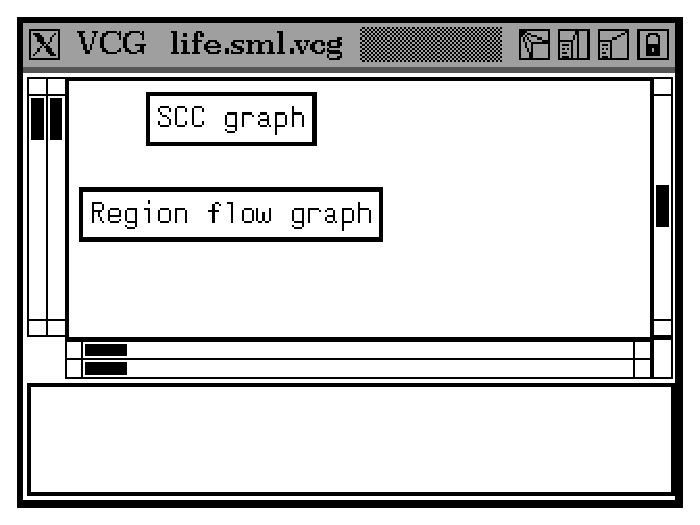
\includegraphics{vcg1.ps}}
\end{center}
\caption{The VCG graph contains two nodes. The
  node ``Region flow graph'' represents the folded region flow graph and
  the node ``SCC graph'' represents the folded strongly connected
  componemt graph.}
\label{vcg1.fig}
\medskip\hrule
\end{figure}

The two graphs are exported \emph{folded}, meaning that they are
represented in the window as one node each. To unfold a graph choose
{\tt Unfold Subgraph} from the pull-down menu inside the {\tt xvcg}
window. The pull-down menu is activated by pressing one of the mouse
buttons. After activating {\tt Unfold Subgraph}, choose with the left mouse button the node
representing the graph that you want to unfold. Then press the right
mouse button to unfold the chosen graph. Figure~\ref{vcg2.fig}
shows a small fraction of the unfolded region flow graph.
\begin{figure}[htb]
%\hrule\medskip
\begin{center}
\scalebox{0.6}{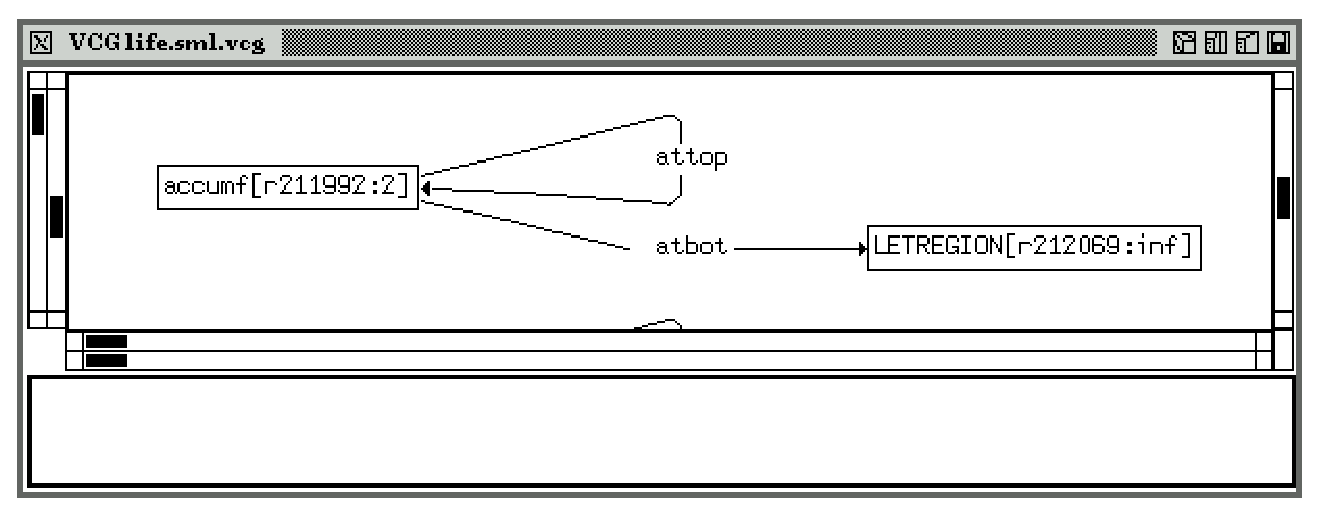
\includegraphics{vcg2.ps}}
\end{center}
\caption{A small fragment of the region flow graph.}
\label{vcg2.fig}
\medskip\hrule
\end{figure}

The graph is read in the same way as the text-based version in the log
file. It can be printed out, scaled, and so on from the pull-down
menu. The graph is folded again by choosing {\tt Fold Subgraph} and
clicking on one of the nodes. All nodes in the graph then turn black;
clicking on the right mouse button then folds the graph.

% Region flow paths are also exported together with the region flow
% graph. Each path is numbered and can be viewed by the {\tt Expose/Hide
%   edges} facility in the VCG pull-down menu, see Figure~\ref{vcg3.fig}.
% \begin{figure}
% \begin{center}
%   \scalebox{0.6}{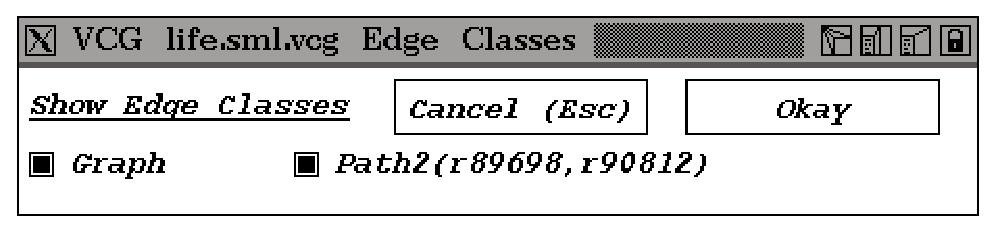
\includegraphics{vcg3.ps}}
% \end{center}
% \caption{After choosing the
%   {\tt Expose/Hide edges} facility you get this window. The window
%   shows that there are two classes of edges in the graph; one for the
%   region flow graph and one for the path from node \texttt{r89698} to node
%   \texttt{r90812}. 
%   %If you have generated the path from Section~\ref{regFlowPath.sec}, the option
%   %\texttt{Path2(r89698,r90812)} is present.
%   }
% \label{vcg3.fig}
% \end{figure}

% Each path is numbered because there can be several paths between the same
% two nodes. Clicking on the {\tt Graph} edge class will hide the edges in the
% region flow graph so that edges in the generated path are the only edges
% shown, see Figure~\ref{vcg4.fig}.
% \begin{figure}
% \begin{center}
%   \scalebox{0.6}{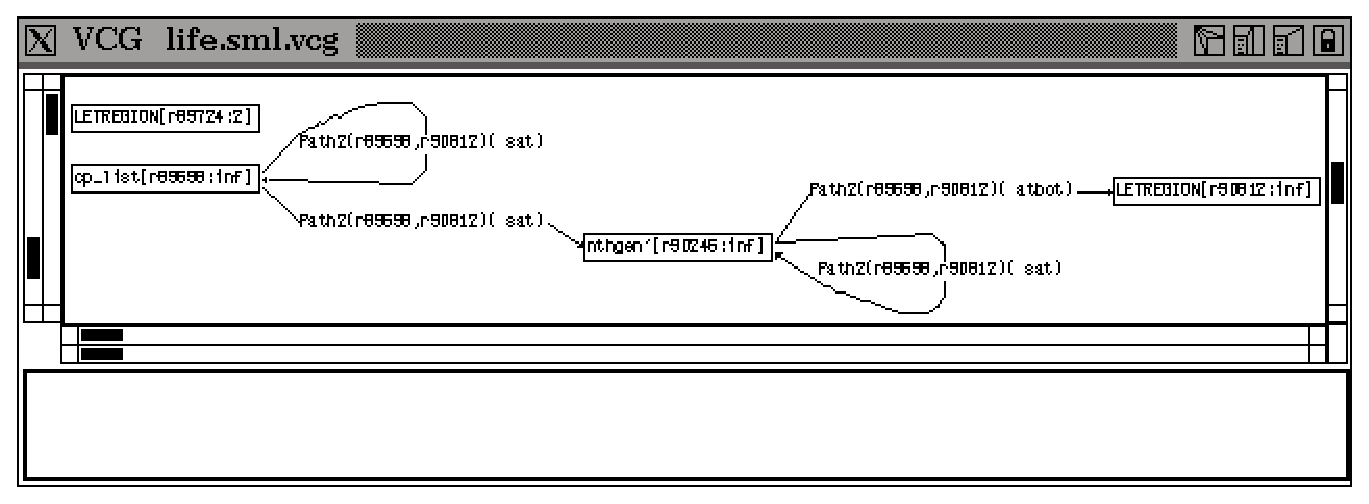
\includegraphics{vcg4.ps}}
% \end{center}
% \caption{The figure shows the path between
%   node \texttt{r89698} and \texttt{r90812}.}
% \label{vcg4.fig}
% \end{figure}

%----------------------------------
\section{Runtime Profiling Strategy}
%----------------------------------
When the source program has been compiled and linked, you have an
executable file, \texttt{run}. Typing \texttt{run} at the command prompt will
execute the program with a predefined 
\index{profile strategy!runtime}%
runtime profiling strategy, which is displayed when the program is
run with the {\tt -verbose} option:
\begin{verbatim}
   ---------------------Profiling-Enabled---------------------
    The profile timer (unix virtual timer) is turned on.
    A profile tick occurs every 1th second.
    Profiling data is exported to file profile.rp.
   -----------------------------------------------------------
\end{verbatim}
You can change the 
\index{profile strategy!options}%
profiling strategy by passing command line arguments directly to the
executable.  The second line says that a virtual timer is used. There
are three possible timers, each of which can be enabled using one of
the following options:\footnote{A complete description can be
    found in the manual page for \texttt{getitimer}.}
\begin{description}
\item[{\tt -realtime}]~
  \index{realtime@\texttt{-realtime} option}%
  \index{timer!real}%
  Real time.
\item[{\tt -virtualtime}]~ 
  \index{virtualtime@\texttt{-virtualtime} option}%
  \index{timer!virtual}%
  The execution time for the process.
\item[{\tt -profiletime}]~
  \index{profiletime@\texttt{-profiletime} option}%
  \index{timer!prof}% 
  The execution time for the process together with the time used in
  the operating system on behalf of the process.
\end{description}

The third line says that a 
\index{profile tick}%
{\em profile tick\/} occurs every 1 second.  A profile tick is when
the program stops normal execution, and memory is traversed to collect
profile data. The more often a profile tick occurs the more detailed
you profile (and the slower the program will run). The
\index{profiling!time slot}%
{\em time slot\/} (i.e., the time between to succeeding profile ticks) to use
is specified by the 
\index{sec@\texttt{-sec} option}%
\texttt{-sec n} and 
\index{microsec@\texttt{-microsec} option}%
\texttt{-microsec n} options. A time slot of half a second is
specified by \texttt{-microsec 500000} and not by \texttt{-sec
  0.5}.\footnote{The lowest possible time slot to use is system
  dependent. 
%  It is also system dependent how long time passes
%  before the time wraps.  Wrapping will in practice not happen on a HP-UX system,
%  but it will happen after about 40 minutes on a SUN OS4 system.
}

The fourth line says that the collected profile data is exported to
the file \texttt{profile.rp}. The default file name setting can be
changed with the
\index{file@\texttt{-file} option}%
\texttt{-file name} option.

There are several other possible command-line options; use the
\texttt{-h} option or the
\index{help@\texttt{-help} option}%
\texttt{-help} option for details. When garbage collection is enabled,
options for controlling garbage collection are also available as
command-line options (see Section~\ref{gc.chap}).

%----------------------------------
\section{Regions Statistics}
%----------------------------------
If the executable file {\tt run} is executed with the option {\tt
  -showStat} then
\index{region statistics}%
{\em region statistics\/} is printed just before the program
terminates. Region statistics includes information about the use of
regions and does not depend on the specifics of the runtime profiling
strategy; in fact, region statistics includes only exact, non-sampled
values for the program. Assuming that {\tt run} is the executable file
generated by compiling the program {\tt life} with profiling enabled,
executing {\tt ./run -showStat} yields---just before the program
terminates---the region statistics shown in
Figure~\ref{region_statistics.fig}.
\begin{figure}
\hrule \medskip
\begin{verbatim}
   MALLOC
     Number of calls to malloc: 2
     Alloc. in each malloc call: 30720 bytes
     Total allocation by malloc: 61440 bytes (0.1Mb)

   REGION PAGES
     Size of one page: 1016 bytes
     Max number of allocated pages: 45
     Number of allocated pages now: 4
     Max space for region pages: 45720 bytes (0.0Mb)

   INFINITE REGIONS
     Size of infinite region descriptor: 16 bytes
     Number of calls to allocateRegionInf: 95764
     Number of calls to deallocateRegionInf: 95761
     Number of calls to alloc: 858816
     Number of calls to resetRegion: 123378
     Number of calls to deallocateRegionsUntil: 0

   ALLOCATION
     Max alloc. space in pages: 17912 bytes (0.0Mb)
       incl. prof. info: 36048 bytes (0.0Mb)
     Infinite regions utilisation (36048/45720): 79%

   STACK
     Number of calls to allocateRegionFin: 1797844
     Number of calls to deallocateRegionFin: 1797844
     Max space for finite regions: 6116 bytes (0.0Mb)
     Max space for region descs: 256 bytes (0.0Mb)
     Max size of stack: 33780 bytes (0.0Mb)
       incl. prof. info: 35660 bytes (0.0Mb)
       in profile tick: 18768 bytes (0.0Mb)
\end{verbatim}
\caption{Region statistics for the {\tt life} program.}
\label{region_statistics.fig}
\medskip\hrule
\end{figure}

The {\tt MALLOC} part of Figure~\ref{region_statistics.fig} shows how
memory is allocated from the operating system.

Each infinite region form a linked list of one or more
\index{region pages}% 
{\em region pages\/} whose size is found in the {\tt REGION PAGES}
part. The value
\begin{verbatim}
   Max number of allocated pages: 45
\end{verbatim}
multiplied by
\begin{verbatim}
   Size of one page: 1016 bytes
\end{verbatim}
gives 
\begin{verbatim}
   Max space for region pages: 45720 bytes (0.0Mb)
\end{verbatim}

In the {\tt INFINITE REGIONS} part, we see the number of calls to
infinite region operations such as {\tt allocateRegionInf} and {\tt
  alloc}. The program allocates 95764 infinite regions and
de-allocates 95761; the three global regions are not de-allocated
before the region statistics is printed and the program terminates.
The program allocates 858816 objects in infinite regions. Infinite
regions has been reset 123378 times. The {\tt deallocateRegionsUntil}
operation is called whenever an exception is raised, thus, we see that
no exceptions were raised by the program.

Because objects allocated in infinite regions are not split across
different region pages (except strings), it is not always possible to
fill out a region page entirely. In the {\tt ALLOCATION} part, the value
\begin{verbatim}
   Infinite regions utilisation (36048/45720): 79%
\end{verbatim}
shows memory utilisation for infinite regions at the moment where the
program has allocated the largest amount of memory in infinite
regions.

In the {\tt STACK} part, we see that the program allocates and
de-allocates the same number of finite regions. We also see that the
space used for finite regions is 6116 bytes and that the total use of
stack space is 33780 bytes (excluding space used to hold profiling
information). The stack size values
\begin{verbatim}
   incl. prof. info: 35660 bytes (0.0Mb)
   in profile tick: 18768 bytes (0.0Mb)
\end{verbatim}
can be used to see if it is necessary to profile with a smaller time
slot, which will often lower the difference between the two values.


%--------------------------------------------
\section{Processing the Profile Data File}
%--------------------------------------------
The profile datafile {\tt profile.rp} can be processed by the 
\index{rp2ps@\texttt{rp2ps} options|(}%
graph generator {\tt rp2ps} (read: RegionProfile2PostScript) found in
the {\tt bin} directory.\footnote{The {\tt rp2ps} program is based on
  a Haskell profiler written by Colin Runciman, David Wakeling and Niklas
  R\"{o}jemo.} The graph generator is controlled by command line
options.

A 
\index{region profile}%
\index{region@\texttt{-region} option}%
region profile is produced by typing
\begin{verbatim}
   rp2ps -region
\end{verbatim}
at the command prompt. The program produces a PostScript file in
file {\tt region.ps} by reading profile information from the 
\index{profile data file}%
profile data file {\tt profile.rp}, see Figure~\ref{profStrategy.fig}.
A region profile for the {\tt life} program is shown in
Figure~\ref{lifeprof80.fig} on page~\pageref{lifeprof80.fig}. The
region that occupies the largest area is at the top. If there are more
regions than can be shown in different shades, then the smallest
regions are collected in an OTHER band at the bottom.

Each region is identified with a number that matches a {\tt
  letregion}-bound region variable in the region-annotated program.
Infinite regions end with {\tt inf} and finite regions end with {\tt
  fin}. There are also a band named {\tt rDesc} and a band named
{\tt stack}. The {\tt rDesc} band shows the memory used on
region descriptors of infinite regions on the stack. The stack band
shows stack usage excluding finite regions and region descriptors for
infinite regions.

The vertical line marked ``Maximum allocated bytes in regions'' in
Figure~\ref{lifeprof80.fig} is called the {\em maximum allocation
  line}; it shows the maximum number of bytes allocated in regions
when the program was executed. Because we also show the stack use on
the graph (as the {\tt rDesc} and {\tt stack} band), the maximum
allocation line is offset upwards by the stack use at the point where
region allocation was at its highest. The space between the maximum
allocation line and the top band shows the inaccuracy of the profiling
strategy. To decrease the gap, it often helps to use a smaller time
slot.

The largest region shown in Figure~\ref{lifeprof80.fig} is {\tt
  r212422}. An
\index{object profile}%
\index{object@\texttt{-object} option}%
object profile of region {\tt r212422} is produced by typing
\begin{verbatim}
   rp2ps -object 212422
\end{verbatim}
at the command prompt. We obtain the object profile shown in
Figure~\ref{prof_eks2.fig}.
\begin{figure}
\begin{center}
\includegraphics{prof_eks2.ps}
\end{center}
\caption{The object profile shows all allocation points allocating into region {\tt r212422}.}
\label{prof_eks2.fig}
\medskip\hrule
\end{figure}

We see that allocation point \texttt{pp29479} is responsible for the
largest amount of allocations in the program. The allocation point may
be found in the region-annotated program resulting from compiling the
{\tt life} program (remember to enable printing of program points). In
general, program points may also stem from the Basis Library (search
the {.log} files in the directory {\tt basislib}).

The stack profile shown in Figure~\ref{prof_eks3.fig} shows memory
usage on the stack, excluding space used by finite regions. A 
\index{stack profile}%
\index{stack@\texttt{-stack} option}%
stack profile is generated by typing
\begin{verbatim}
   rp2ps -stack
\end{verbatim}
at the command prompt.

\begin{figure}
\begin{center}
\includegraphics{prof_eks3.ps}
\end{center}
\caption{Memory usage on the stack excluding space for finite regions.}
\label{prof_eks3.fig}
\medskip\hrule
\end{figure}

%-------------------------------------------------------
\section{Advanced Graphs with \texttt{rp2ps}}
%-------------------------------------------------------
This section gives a quick overview of the more advanced options that can
be passed to \texttt{rp2ps}. First of all, it is possible to name the
profiles with the 
\index{name@\texttt{-name} option}%
{\tt -name} option. Comments are inserted on the
x-axis with the 
\index{comment@\texttt{-comment} option}%
{\tt -comment} option.

The profile data file may contain a large number of \emph{samples}
(the data collected by a profile tick is called a sample). By default,
\texttt{rp2ps} uses only 64 samples. You can alter the setting with the
\index{sampleMax@\texttt{-sampleMax} option}%
\texttt{-sampleMax} option. The following two algorithms are used to sort
out samples:
\begin{description}
\item[{\tt -sortBySize}]~
  \index{sortBySize@\texttt{-sortBySize} option}%
  The $n$ (specified by \texttt{-sampleMax}) largest samples are
  shown.
\item[{\tt -sortByTime}]~
  \index{sortByTime@\texttt{-sortByTime} option}%
  The $n$ samples shown are equally distributed over time (default).
\end{description}
The \texttt{-sortBySize} option is useful if your profiles have a
large gap between the top band and the maximum allocation line.  If
there is a large gap when using option \texttt{-sortBySize}, then it
may help to profile with a smaller time slot. You can use the
\index{stat@\texttt{-stat} option}%
{\tt -stat} option to see the number of samples in the profile data
file. It is printed as \texttt{Number of ticks:}.

Figure~\ref{prof_eks4.fig} shows the profile for the following
command line:
\begin{verbatim}
   rp2ps -region -sampleMax 50 -name life \
         -comment 0.6 "A comment at time 0.6" -sortBySize
\end{verbatim}

\begin{figure}
\begin{center}
  \includegraphics{prof_eks4.ps}
\end{center}
\caption{It is possible to insert comments in profile graphs.}
\label{prof_eks4.fig}
\medskip\hrule
\end{figure}

The graph generator recognises several options that are not mentioned
here. Help on these options is obtained by typing \texttt{rp2ps -h} or
\index{help@\texttt{-help} option}%
{\tt rp2ps -help} at the command prompt.
\index{rp2ps@\texttt{rp2ps} options|)}%

%---------------------------------------------------------
\chapter{Interacting with the Kit}
\label{controlkit.sec}
\label{startup.sec}
%---------------------------------------------------------

Starting the Kit was described in Section~\ref{tryit.sec}.  To
\index{leaving the Kit}%
\index{exit from the Kit}%
\index{quitting from the Kit}%
leave the Kit, type 
\index{quit@\texttt{quit}}%
\boxml{quit} followed by a return character.

We have already described how to compile and run single source files
(Section~\ref{tryit.sec}) and projects
(Chapter~\ref{modules_and_projects.chap}).  In the following sections,
we give an overview of the Kit sub-menus that control printing and
layout of intermediate forms. In Section~\ref{scriptfiles.sec}, we
explain how to use a so-called script file to set personal preferences
for menu entries in the Kit. The settings that can be controlled using
the menu and script files can also be controlled using command-line
options to the ML Kit executables. One useful command-line option is
the 
\index{help@\texttt{-help} option to \texttt{mlkit}}%
{\tt -help} option; Appendix~\ref{mlkithelp.app} shows the output of
executing \boxml{mlkit -help} in a version of the Kit that uses the
native x86 backend.



%------------------------------------------------
\section{Printing of Intermediate Forms}
\label{printing_intermediate_forms.sec}
%------------------------------------------------
The menu 
\index{Printing of intermediate forms@\texttt{Printing of intermediate forms}}%
\texttt{Printing of intermediate forms} controls what intermediate
forms are printed when a program is compiled.
A summary of the major phases that produce printable intermediate
forms is shown in Figure~\ref{phases.fig}. The phases are listed in
the order they take place in the Kit.
\begin{figure}
\begin{center}
\begin{tabular}{|l|l|l|}
\hline
 {\bf Phase} & {\bf Result} & {\bf Flag(s) that Print Result} \\
\hline
 Elaboration            & $\Lam$    & \hfill \boxml{$(\ast)$}\\
 Elim. of Poly. Eq.     & $\Lam$    & \hfill \boxml{$(\ast)$}\\
 Lambda Optimiser       & $\Lam$    & \boxml{print optimised}\\&&~~\boxml{lambda expression} \hfill $(\ast)$\\
 Spreading              & $\RegExp$ & \hfill \boxml{$(\ast)$}\\
 Region Inference       & $\RegExp$ & \hfill \boxml{$(\ast)$}\\
 Multiplicity Inference & $\MulExp$ & \hfill \boxml{$(\ast)$}\\
 K-normalisation        & $\MulExp$ & \\
 Storage Mode Analysis  & $\MulExp$ & \boxml{print storage mode}\\&&~~\boxml{expression} \hfill $(\ast)$\\
 Dropping of Regions    & $\MulExp$ & \boxml{print drop regions}\\&&~~\boxml{expression} \hfill $(\ast)$\\
                        &           & \boxml{print drop regions}\\&&~~\boxml{expression with}\\&&~~\boxml{storage modes} \\
 Physical Size Inference& $\MulExp$ & \boxml{print physical size}\\&&~~\boxml{inference expression} \hfill $(\ast)$\\
 Call Conversion        & $\MulExp$ & \boxml{print call-explicit}\\&&~~\boxml{expression} \hfill $(\ast)$\\
\hline
\end{tabular}
\end{center}
\caption{The table shows how the menu items in the 
  \index{intermediate forms}%
  {\tt Printing of Intermediate Forms} menu correspond to the phases
  in the Kit.  Enabling \boxml{debug compiler} from the \boxml{Debug
    Kit} menu causes all intermediate forms marked $(\ast)$ to be
  printed.  Thus, one can select phases individually or ask to have all
  printed.  The phases that follow K-normalisation all work on
  K-normal forms, but, for readablity, terms are printed as though
  they had not been normalised (unless \boxml{Print in K-normal Form}
  from the {\tt Layout} menu is enabled).}
\label{phases.fig}
\end{figure}

The optimiser, which rewrites a $\Lam$\index{Lambda@$\Lam$}
program, collects statistics about the optimisation. This statistics
can be printed by turning on the flag
\index{statistics after optimisation@\texttt{statistics after optimisation}}%
\index{optimisation!statistics}%
\texttt{statistics after optimisation} in the
\texttt{Control/Optimiser} menu; the other flags found in this menu
controls the optimiser.

Storage mode analysis (see Chapter~\ref{storagemodes.sec}) results in
a $\MulExp$\index{MulExp@$\MulExp$} expression, which can be printed
by turning on the flag
\index{print storage mode expression@\texttt{print storage mode expression}}%
\texttt{print storage mode expression}.  After that, region parameters
for which there are only $\Get$ effects on in the type scheme for a
region polymorphic function are removed from the $\MulExp$ expression
(see page~\pageref{bother-to-distinguish-get-n-put}).  To see the
resulting expression, turn on
\index{print drop regions expression@\texttt{print drop regions expression}}%
\texttt{print drop regions expression} or \texttt{print drop regions
  expression with storage modes}. (The latter flag also prints storage
modes.)
\index{physical size inference}%
\index{region size}%
Physical size inference then determines the size in words of finite
region variables.  For instance, a finite region that will contain a
pair will have physical size two words.  To see the expression after
physical size inference, turn on
\index{print physical size inference expression@\texttt{print physical size inference expression}}%
\texttt{print physical size inference expression}.  After that,
\index{call conversion}%
call conversion converts the $\MulExp$ expression to a
\index{expression!call-explicit}call-explicit expression (see
page~\pageref{call-explicit}).  To see the result, enable the flag
\texttt{print call-explicit expression}.  

After that, dependent on which backend is used, either 
\index{backend!native}%
native machine code or bytecode is generated. If you use the native
backend you can inspect the code at different steps of the
transformation into machine code by toggling entries in the
\texttt{Printing of intermediate forms} menu. Similarly, if you use
the
\index{backend!bytecode}%
bytecode backend, toggling of entries in the \texttt{Printing of
  intermediate forms} menu allows you to inspect the bytecode
generated by the Kit.

\section{Layout of Intermediate Forms}
\label{layout_intermediate_forms.sec}
While the switches described in the previous section concern which
intermediate forms to print, the switches in the sub-menu
\texttt{Layout}\index{Layout@\texttt{Layout}} control how these forms
are printed.

The flags 
\index{print types@\texttt{print types}}%
\texttt{print types},
\index{print effects@\texttt{print effects}}%
\texttt{print effects}, and
\index{print regions@\texttt{print regions}}%
\texttt{print regions} control the printing of region-annotated types,
effects, and region allocation points (e.g., $\at\,\rho$).
All eight combinations of these three flags are possible, but if
\index{print effects@\texttt{print effects}}%
{\tt print effects} is turned on it is best also to turn the two
others on so that one can see where the effect variables and region variables
that appear in arrow effects are bound.

Enabling the flag
\index{print in K-Normal Form@\texttt{print in K-Normal Form}}%
\texttt{print in K-Normal Form}
\index{K-normalisation}%
causes expressions to be output in K-Normal Form instead of the
simplified form in which they are normally presented.

\section{Using Script Files for Preferences}
\label{scriptfiles.sec}
The Kit allows you to create a so-called 
\index{script file}%
{\em script file}, which can hold preferences for most of the entries
found in the Kit menu. A script file can be provided either when the
Kit is started or dynamically from within the Kit menu when the Kit is
running. To provide a script file {\tt script} at the time the Kit is
started, type
\begin{verbatim}
   mlkit -script script
\end{verbatim}
from the shell. During a session with the Kit, a script file can be
read using the menu entry {\tt Read a script file} from the {\tt File}
menu.

A script file is comprised by a sequence of 
\index{preferences}%
{\em preferences}, each of which provides a setting for a given entry.
Here is a script file that enables the boolean entry {\tt print drop
  regions expression} (located in the {\tt Printing of intermediate
  forms} sub-menu) and sets the integer entry {\tt maximum inline
  size} (located in the sub-menu {\tt Control/Optimiser}) to {\tt
  0}:\footnote{Script file {\tt kitdemo/ex.script}.}
\begin{verbatim}
   val print_drop_regions_expression : bool = true 
   val maximum_inline_size : int = 0  (* disable in-lining *)
\end{verbatim}
Notice that spaces in the menu entries are replaced with scores in the
script file and that script files may include ML style comments. By
selecting {\tt print all flags and variables} from the {\tt Control}
sub-menu, the Kit prints a table of all entries that may be set from a
script file.

Enabling 
\index{print in K-Normal Form@\texttt{print in K-Normal Form}}%
\index{K-normalisation}%
\texttt{print in K-Normal Form} causes expressions to be output in
K-Normal Form instead of the simplified form in which they are
normally presented.


%---------------------------------------------------------
\chapter{Calling C Functions}
\label{ccall.sec}
%---------------------------------------------------------

In this chapter, we describe how the Kit programmer can call 
\index{C!calling}%
C functions from within Standard ML programs.  The Kit allows ML
values to be passed to C functions, which again may return ML values.
Not all ML values are represented as if they were C values. For
instance, C strings are null-terminated arrays of characters, whereas
ML strings in the Kit are represented as a linked list of bounded
sized character arrays. To allow the programmer to conveniently
convert between C values and ML values, the Kit provides conversion
functions and macros for commonly used data structures.

When the Kit calls a C function, data structures returned by the
function are stored in regions that are allocated by the Kit. For
dynamically sized objects of the resulting value, such as strings and
lists, regions are allocated by the Kit and passed to the C function
as additional arguments; the C function must then itself allocate
space in these regions for the dynamically sized data
structures. Moreover, for those parts of the resulting value for which
the size can be determined statically, pointers to already allocated
space are passed to the C function as additional arguments.

In both cases, the Kit uses region inference to infer the lifetime of
regions that are passed to the C function.  The region inference
algorithm does not analyse C functions. Instead, the Kit inspects the
ML type provided by the programmer. The Kit assumes that functions
with monomorphic types are 
\index{region exomorphism}%
region exomorphisms;
\index{region endomorphism}%
region endomorphic functions may be described using ML polymorphism,
see Section~\ref{C_polymorphism.sec}.

For every C function that is called from an ML program, the order of the
additional region arguments is uniquely determined by the ML result type
of the function.  This type must be constructed from lists, records,
booleans, reals, strings, integers, and type variables.

When profiling is enabled, yet another additional argument, a program
point, is passed to the C function. This argument provides allocation
primitives with information about what points in the program
contributes with allocation, see Section~\ref{prof.sec}.

Examples of existing libraries that can be accessed from within ML
programs include the X Window System and standard UNIX libraries
providing functions such as {\tt time}, {\tt cp}, and {\tt
fork}. There are limitations to the scheme, however. First, because C
and the Kit do not share value representations, transmitting large
data structures between C and ML will often involve significant
copying. Second, some C libraries require the user to set up
\index{call-back function}%
call-back functions to be executed when specific events occur. It is
not currently possible with the Kit to have a C function call an ML
function.

%========================================================
\section{Declaring Primitives and C Functions}
\label{parPassing.sec}
%========================================================
The Kit conforms in large parts to the Standard ML Basis Library. Part
of the functionality found in this library is programmed in C and
linked to the Kit runtime system.  The declarations in system
dependent parts of the library use a special built-in identifier
called \index{prim@\texttt{prim}}\texttt{prim}, which is declared to have type
scheme $\forall \alpha \beta .  \texttt{string} 
\ast \alpha \rightarrow \beta$ in the initial basis.  A primitive
function is then declared by passing its name to \texttt{prim}.  For
example, the declaration
\begin{verbatim}
   fun (s : string) ^ (s' : string) : string = 
     prim ("concatString", (s, s'))
\end{verbatim}
declares string catenation.  The argument and result types are
explicitly stated so as to give the primitive the correct type scheme.
The string \boxml{"concatString"} denotes a C function
identifier.\footnote{Some primitives (e.g., \boxml{"="} and
  \boxml{":="}) are recognised and implemented in assembler by the
  compiler.} For the example declaration, the Kit generates a call to
the C function \boxml{concatString} with arguments {\tt s} and {\tt
  s'}. The C function must then of course be present at link-time; if
not, the Kit complains.\footnote{When profiling is enabled, the Kit
  automatically appends the extension \texttt{Prof} for those
  functions that take regions (and thus a program point) as argument;
  see Section~\ref{prof.sec}.}%
A convenient way to declare a C function is to use the following
scheme:
$$\texttt{fun}~ \emph{vid} ~\texttt{(}x_1:\tau_1, \ldots, x_n:\tau_n\texttt{)}
    : \tau ~\texttt{=} ~\texttt{prim(}\emph{c\_func}, \texttt{(}
  x_1, \ldots, x_n\texttt{)} \texttt{)}
$$
The result type $\tau$ must be of the form
\begin{quote}
\begin{tabbing}
$\tau$ ::\== ~\= $\alpha$ $~|~$ {\tt int} $~|~$ {\tt bool} $~|~$ {\tt unit} \\ 
  \> $|$ \> $\tau_1 \ast \ldots \ast \tau_n$ $~|~$ $\tau$ {\tt list} $~|~$ {\tt real} $~|~$ {\tt string} 
\end{tabbing}
\end{quote}
\noindent
If the result type is one of $\alpha$, {\tt int}, {\tt bool}, or ${\tt unit}$ then the
result value can be returned in a single register. Contrary, if the result type represents an allocated
value, the C function must be told where to store the value. For
any type that is either {\tt real} or a non-empty tuple type, and
does not occur in a list type of the result type $\tau$, the Kit
allocates space for the value and passes a pointer to the allocated
space as an additional argument to the C function. For any type
representing an allocated value that is either {\tt string} or occurs in a
list type of the result type $\tau$, the Kit cannot statically
determine the amount of space needed to store the value. Instead,
regions are passed to the C function as additional arguments and the C
function must then explicitly allocate space in these regions as
needed, using a C function provided by the runtime system. The order
in which these additional arguments are passed to the C function is determined
by a pre-order traversal of the result type $\tau$.  For a list type,
regions are given in the order:
\begin{enumerate}
    \item region for auxiliary pairs
    \item regions for elements (if necessary)
\end{enumerate}

We now give an example to show what extra arguments are passed to a
C function, given the result type. In the example, we use the following
(optional) naming convention: 
names of arguments holding addresses of 
pre-allocated space in regions 
start with {\tt vAddr}, while names of arguments
holding addresses of region descriptors (to be used for allocation in a
region) start with {\tt rAddr}.
\begin{example}
  Given the result type $({\tt int} \ast {\tt string}) ~{\tt list}
  \ast {\tt real}$, the following extra ar\-gu\-ments are passed to the
  C function (in order): {\tt vAddrPair},
  {\tt rAddrLPairs}, {\tt rAddrEPairs}, {\tt rAddrEStrings} and {\tt
    vAddrReal}, see Figure \ref{args_ex1.fig}. 
  
  Here {\tt vAddrPair} holds an address pointing to pre-allocated
  storage in which the tuple of the list and the (pointer to the) real
  should reside. The argument {\tt rAddrLPairs} holds the region
  address for the auxiliary pairs of the list. Similarly, the
  arguments {\tt rAddrEPairs} and {\tt rAddrEStrings} hold region
  addresses for element pairs and strings, respectively. The argument
  {\tt vAddrReal} holds the address for pre-allocated storage for the
  real.
\end{example}

\setlength{\unitlength}{1pt}
\begin{figure}
\hrule
\begin{center}
\begin{picture}(400,155)
\put(125,140){\framebox{$\ast$}}
\put(155,100){\framebox{\texttt{real}}}
\put(75,100){\framebox{\texttt{list}}}
\put(85,60){\framebox{$\ast$}}
\put(40,20){\framebox{\texttt{int}}}
\put(115,20){\framebox{\texttt{string}}}
\put(125,140){\line(-1,-1){29}}
\put(138,140){\line(1,-1){29}}
\put(90,97){\line(0,-1){28}}
\put(85,60){\line(-1,-1){29}}
\put(98,60){\line(1,-1){29}}

\put(115,145){\circle{10}}\put(115,145){\makebox(0,0){1}}
\put(65,105){\circle{10}}\put(65,105){\makebox(0,0){2}}
\put(75,65){\circle{10}}\put(75,65){\makebox(0,0){3}}
\put(30,25){\circle{10}}\put(30,25){\makebox(0,0){4}}
\put(105,25){\circle{10}}\put(105,25){\makebox(0,0){5}}
\put(145,105){\circle{10}}\put(145,105){\makebox(0,0){6}}

\put(200,145){\circle{10}}\put(200,145){\makebox(0,0){1}}
\put(210,142){\texttt{vAddrPair}}

\put(200,125){\circle{10}}\put(200,125){\makebox(0,0){2}}
\put(210,122){\texttt{rAddrLPairs}}

\put(200,105){\circle{10}}\put(200,105){\makebox(0,0){3}}
\put(210,102){\texttt{rAddrEPairs}}

\put(200,85){\circle{10}}\put(200,85){\makebox(0,0){4}}
\put(210,82){Integers are unboxed}

\put(200,65){\circle{10}}\put(200,65){\makebox(0,0){5}}
\put(210,62){\texttt{rAddrEStrings}}

\put(200,45){\circle{10}}\put(200,45){\makebox(0,0){6}}
\put(210,42){\texttt{vAddrReal}}

\end{picture}
\caption{The order of pointers to allocated space and infinite regions
  is determined from a pre-order traversal of the result type $({\tt
  int} \ast {\tt string}) ~{\tt list} \ast {\tt real}$.}
\label{args_ex1.fig}
\end{center}
\hrule
\end{figure}

Additional arguments holding pointers to pre-allocated space and
infinite regions are passed to the C function prior to the ML
arguments. Consider again the ML declaration
$$\texttt{fun}~ \emph{vid} ~\texttt{(}x_1:\tau_1, \ldots, x_n:\tau_n\texttt{)}
    : \tau ~\texttt{=} ~\texttt{prim(}\emph{c\_func}, \texttt{(}
  x_1, \ldots, x_n\texttt{)} \texttt{)}
$$
\noindent
The C function \emph{c\_func} must then be declared as
\begin{eqnarray}
  \texttt{int} \ \emph{c\_func} \ \texttt{(}\texttt{int}\ \emph{addr}_1,
    \ldots, \texttt{int}\ \emph{addr}_m,\ \texttt{int}\ x_1, \ldots, \texttt{int}\ x_n\texttt{)} \nonumber
\end{eqnarray}
\noindent
where \emph{addr}$_1$, $\ldots$, \emph{addr}$_m$ are pointers to
pre-allocated space and infinite regions as described above.


%========================================
\section{Conversion Macros and Functions}
%========================================
The runtime system provides a small set of conversion macros and
functions for use by C functions that need to convert between ML
values and C values. Using these conversion macros and functions for
converting between representations protects you against future
changes in the representation of ML values. The conversion macros and
functions are declared in the header
files:\index{Tagging.h@\texttt{Tagging.h}}\index{String.h@\texttt{String.h}}
\begin{verbatim}
   src/Runtime/Tagging.h
   src/Runtime/String.h
   src/Runtime/List.h
\end{verbatim}

%--------------------
\subsection{Integers}
%--------------------
There are two macros for converting between the ML representation of
integers and the C representation of integers:\footnote{These macros are the identity maps when garbage collection is disabled.}
\index{convertIntToC@\texttt{convertIntToC}}%
\index{convertIntToML@\texttt{convertIntToML}}%
\begin{verbatim}
   #define convertIntToC(i)
   #define convertIntToML(i)
\end{verbatim}
To convert an ML integer \verb|i_ml| to a C integer \verb|i_c|,
write 
\begin{verbatim}
   i_c = convertIntToC(i_ml);
\end{verbatim}
To convert a C integer \verb|i_c| to an ML
 integer \verb|i_ml|, write
\begin{verbatim}
   i_ml = convertIntToML(i_c);
\end{verbatim}
The macros demonstrated here are used in the examples~\ref{power.ex},
\ref{power_real.ex}, and~\ref{power_exn.ex} in Section~\ref{Cexamples.sec}.

%-----------------
\subsection{Units}
%-----------------
The following constant in the conversion library denotes the ML
representation of {\tt ()}:
\index{mlUNIT@\texttt{mlUNIT}}%
\begin{verbatim}
   #define mlUNIT
\end{verbatim}

%-----------------
\subsection{Reals}
%-----------------
An ML real is represented as a pointer into a region containing the
real. To convert an ML real to a C real, we dereference the pointer. To
convert a C real to an ML real, we update the memory to contain the C
real. The following two macros are provided:
\index{convertRealToC@\texttt{convertRealToC}}%
\index{convertRealToML@\texttt{convertRealToML}}%
\begin{verbatim}
   #define convertRealToC(mlReal)
   #define convertRealToML(cReal, mlReal)
\end{verbatim}

Converting an ML real \verb|r_ml| to a C real \verb|r_c| can be done with the first macro:
\begin{verbatim}
   r_c = convertRealToC(r_ml);
\end{verbatim}

Converting from a C real to an ML real (being part of the result value of the
C function) is done in one or two steps depending on whether the real is
part of a list or not. If the real is not in a list the memory containing
the real has been allocated before the C call, see Section~\ref{parPassing.sec}:
\begin{verbatim}
   convertRealToML(r_c, r_ml);
\end{verbatim}
If the ML real is part of a list element, then space must be allocated for
the real before converting it. If \boxml{rAddr} identifies a region
for the real, you write:
\index{allocReal@\texttt{allocReal}}%
\begin{verbatim}
   allocReal(rAddr, r_ml);
   convertRealToML(r_c, r_ml);
\end{verbatim}

These macros are used in the examples~\ref{power_real.ex},
\ref{power_exn.ex} and~\ref{real_list.ex} in
Section~\ref{Cexamples.sec}.

%--------------------
\subsection{Booleans}
%--------------------
Four constants provide the values of true and false in ML and in C.
These constants are defined by the following macros:\footnote{For
  historical reasons, booleans in the Kit are tagged even when garbage
  collection is disabled.}
\index{mlTRUE@\texttt{mlTRUE}}%
\index{mlFALSE@\texttt{mlFALSE}}%
\index{cTRUE@\texttt{cTRUE}}%
\index{cFALSE@\texttt{cFALSE}}%
\begin{verbatim}
   #define mlTRUE  3
   #define mlFALSE 1
   #define cTRUE   1
   #define cFALSE  0
\end{verbatim}

Two macros are provided for converting booleans:
\index{convertBoolToC@\texttt{convertBoolToC}}%
\index{convertBoolToML@\texttt{convertBoolToML}}%
\begin{verbatim}
   #define convertBoolToC(i)
   #define convertBoolToML(i)
\end{verbatim}
Converting booleans is similar to converting integers:
\begin{verbatim}
   b_c = convertBoolToC(b_ml);
   b_ml = convertBoolToML(b_c);
\end{verbatim}

%-------------------
\subsection{Records}
%-------------------
Records are boxed. One macro is provided for storing and retrieving
elements:
\index{elemRecordML@\texttt{elemRecordML}}%
\begin{verbatim}
   #define elemRecordML(recAddr, offset)
\end{verbatim}
An element can be retrieved from a record \verb|rec_ml| by writing 
\begin{verbatim}
   e_ml = elemRecordML(rec_ml, offset);
\end{verbatim}
where the first element has \boxml{offset} 0. An element \verb|e_ml|
is stored in an ML record \verb|rec_ml| by writing
\begin{verbatim}
   elemRecordML(rec_ml, offset) = e_ml;
\end{verbatim}
Two specialized versions of the \boxml{elemRecordML} macro are
provided for 
\index{first@\texttt{first}}%
\index{second@\texttt{second}}%
pairs:
\begin{verbatim}
   #define first(x)
   #define second(x)
\end{verbatim}

If the record is to be part of a list element then it is necessary to allocate the record
before storing into it. This allocation is done with the macro
\index{allocRecordML@\texttt{allocRecordML}}%
\begin{verbatim}
   #define allocRecordML(rAddr, size, vAddr)
\end{verbatim}
where \boxml{rAddr} denotes a region (i.e., a pointer to a region
descriptor), \boxml{size} is the size of the record (i.e., the number
of components), and \boxml{vAddr} is a variable in which
\boxml{allocRecordML} returns a pointer to storage for the record. The
record is then stored, component by component, by repeatedly calling
\boxml{elemRecordML} with the pointer \boxml{vAddr} as argument.

The above macros are used in examples~\ref{real_list.ex},
\ref{change_elem.ex} and~\ref{dir.ex} in Section~\ref{Cexamples.sec}.

%-------------------
\subsection{Strings}
%-------------------
Strings are boxed and always allocated in infinite regions. It is possible
to print an ML string by using the C function
\index{printString@\texttt{printString}}%
\begin{verbatim}
   void printString(StringDesc *str);
\end{verbatim}

Strings are converted from ML to C and vice versa using the two C 
functions
\index{convertStringToC@\texttt{convertStringToC}}%
\index{convertStringToML@\texttt{convertStringToML}}%
\begin{verbatim}
   void convertStringToC(StringDesc *mlStr, char *cStr, 
                         int cStrLen, int exn);
   StringDesc *convertStringToML(int rAddr, char *cStr);
\end{verbatim}
An ML string \verb|str_ml| is converted to a C
string \verb|str_c| in already allocated storage of size \boxml{size} bytes by writing
\begin{verbatim}
   convertStringToC(str_ml, str_c, size, exn);
\end{verbatim}
where \boxml{exn} is some ML exception value (see
Section~\ref{C_exceptions.sec}) to be raised if the ML string has size
greater than \boxml{size}.  

A C string is converted to an ML string in the region denoted by
\boxml{rAddr} by writing
\begin{verbatim}
   str_ml = convertStringToML(rAddr, str_c);
\end{verbatim}

The following function returns the size of an ML string:
\index{sizeString@\texttt{sizeString}}%
\begin{verbatim}
   int sizeString(StringDesc *str);
\end{verbatim}

These macros are used in the examples~\ref{dir.ex} and
\ref{print_string_list.ex} in Section~\ref{Cexamples.sec}.

%-----------------
\subsection{Lists}
%-----------------

Lists are always allocated in infinite regions. A list uses, as a minimum,
one region for the auxiliary pairs of the list, see Figure~\ref{listregions.fig} on page~\pageref{listregions.fig}.

We shall now show three examples of manipulating lists. The first example
traverses a list. Consider the following C function template:
\index{traverse_list@\texttt{traverse\_list}}%
\begin{verbatim}
   void traverse_list(int ls) {
     int elemML;
     for ( ; isCONS(ls); ls=tl(ls)) {
       elemML = hd(ls);
       /*do something with the element*/
     }
     return;
   }
\end{verbatim}

The ML list is passed to the C function in parameter \texttt{ls}.
The example uses a simple loop to traverse the list. The parameter
\texttt{ls} points at the first constructor in the list. Each time
we have a \texttt{CONS} constructor we also have an element, see
Figure~\ref{listregions.fig}. The element can be retrieved with the
\texttt{hd} macro.  One retrieves the tail of the list by using the
\texttt{tl} macro.

The following four macros are provided in the {\tt src/Runtime/List.h}
header file:
\index{isNIL@\texttt{isNIL}}%
\index{isCONS@\texttt{isCONS}}%
\index{hd@\texttt{hd}}%
\index{tl@\texttt{tl}}%
\begin{verbatim}
   #define isNIL(x)
   #define isCONS(x)
   #define hd(x)
   #define tl(x)
\end{verbatim}
                                
The next example explains how to construct a list backwards. Consider
the following C function template:
\index{mk_list_backwards@\texttt{mk\_list\_backwards}}%
\begin{verbatim}
   int mk_list_backwards(int pairRho) {
     int *resList, *pair;
     makeNIL(resList);  
     while (/*more elements*/) {
       ml_elem = ...;
       allocRecordML(pairRho, 2, pair);
       first(pair) = (int) ml_elem;
       second(pair) = (int) resList;
       makeCONS(pair, resList);
     }
     return (int) resList;
   }
\end{verbatim}
First, we create the \texttt{NIL} constructor, which marks the end of
the list. Then, each time we have an element, we allocate a pair. We
store the element in the first cell of the pair. A pointer to the list
constructed so far is put in the second cell of the pair. (In this
release of the Kit, the \boxml{makeCONS} macro simply assigns its
second argument the value of its first argument.) In the example, we
have assumed that the elements are unboxed, thus, no regions are
necessary for the elements.

The last example shows how a list can be constructed forwards. It is more
clumsy to construct the list forwards because we have to return a pointer
to the first element. Consider the following C function template.
\index{mk_list_forwards@\texttt{mk\_list\_forwards}}%
\begin{verbatim}
   int mk_list_forwards(int pairRho) {
     int *pair, *cons, *temp_pair, res;

     /* The first element is special because we have to    */
     /* return a pointer to it.                            */
     ml_elem = ...
     allocRecordML(pairRho, 2, pair);
     first(pair) = (int) ml_elem;
     makeCONS(pair, cons);
     res = (int) cons;

     while (/*more elements*/) {
       ml_elem = ...
       allocRecordML(pairRho, 2, temp_pair);
       first(temp_pair) = (int) ml_elem;
       makeCONS(temp_pair, cons);
       second(pair) = (int) cons;
       pair = temp_pair;
     }
     makeNIL(cons);
     second(pair) = (int)cons;
     return res;
   }
\end{verbatim}

We create the \texttt{CONS} constructor and pair for the first element
and return a pointer to the \texttt{CONS} constructor (the pair) as
the result. We then construct the rest of the list by constructing a
\texttt{CONS} constructor and a pair for each element. It is necessary
to use a temporary variable for the pair (\verb|temp_pair|) because we
have to update the pair for the previous element. The second component
of the last pair contains the \texttt{NIL} constructor and thus
denotes the end of the list.

The two macros \texttt{makeCONS} and \texttt{makeNIL} are provided in
the \boxml{List.h} header file:
\index{makeNIL@\texttt{makeNIL}}%
\index{makeCONS@\texttt{makeCONS}}%
\begin{verbatim}
   #define makeNIL(rAddr, ptr)
   #define makeCONS(rAddr, pair, ptr)
\end{verbatim}

%=======================================================
\section{Exceptions}
\label{C_exceptions.sec}
%=======================================================
C functions are allowed to raise exceptions and it is possible for the
ML code to handle these exceptions. A C function cannot declare
exceptions locally, however. As an example, consider the ML
declaration:
\begin{verbatim}
   exception Exn
   fun raiseif0 (arg : int) : unit = 
     prim("raiseif0", (arg, Exn))
\end{verbatim}
If we want the function \texttt{raiseif0} to raise the exception value
\texttt{Exn} if the argument (\texttt{arg}) is 0 then we use the
function \verb|raise_exn| provided by the runtime system, by
including the header file {\tt src/Runtime/Exception.h}. The C
function \boxml{raiseif0} may be defined thus:
\begin{verbatim}
   void raiseif0(int i_ml, int exn) {
     int i_c;
     i_c = convertIntToC(i_ml);
     if (i_c == 0) raise_exn(exn);
     return;
   }
\end{verbatim}
There is no need to make the function return the value \boxml{mlUNIT};
in case the type of the return value is \boxml{unit} then the Kit
automatically inserts code for returning the ML value \boxml{()} after
the call to the C function.

Exceptions are used in examples~\ref{power_exn.ex} and~\ref{dir.ex} in
Section~\ref{Cexamples.sec}.

%=======================================================
\section{Program Points for Profiling}
\label{prof.sec}
%=======================================================
To support profiling, the programmer must provide special profiling
versions of those C functions that allocate space in regions (i.e.,
that take regions as additional arguments). If profiling is enabled
and at least one pointer to a region is passed to the C function then
also a program point that represents the call to the C function is
passed.  The program point is used by the C function when allocating
space in regions, as explained in Section~\ref{prof.sec}. The program
point is passed as the last argument:
\begin{tabbing}
\indent\=  $\texttt{int} \ \emph{c\_funcProf} \ ($\=$\texttt{int}\ \emph{addr}_1,
    \ldots, \texttt{int}\ \emph{addr}_m,$\\
  \>\>$ \texttt{int}\ x_1, \ldots,
    \texttt{int}\ x_n, \texttt{int}\ \emph{pPoint}) $
\end{tabbing}
\noindent
No special version of the C function is needed if it does not allocate
into infinite regions; in this case, the same C function can be used
both when profiling is enabled and disabled.

A program point passed to a C function is an integer; it identifies the
allocation point that represents the C call in the program, see
Chapter~\ref{useOfProf.sec}.

The runtime system provides special versions of various allocation
macros and functions presented earlier in this chapter:
\index{allocRealProf@\texttt{allocRealProf}}%
\index{allocRecordMLProf@\texttt{allocRecordMLProf}}%
\index{convertStringToMLProf@\texttt{convertStringToMLProf}}%
\begin{verbatim}
   #define allocRealProf(realRho, realPtr, pPoint)
   #define allocRecordMLProf(rhoRec, ssize, recAddr, pPoint)
   StringDesc *convertStringToMLProf(int rhoString, 
                                     char *cStr, 
                                     int pPoint);
\end{verbatim}

Here is the profiling version of the C function
\verb|mk_list_backwards|:
\begin{verbatim}
   int mk_list_backwardsProf(int pairRho, int pPoint) {
     int *resList, *pair;
     makeNIL(resList);  
     while (/*more elements*/) {
       ml_elem = ...;
       allocRecordMLProf(pairRho, 2, pair, pPoint);
       first(pair) = (int) ml_elem;
       second(pair) = (int) resList;
       makeCONS(pair, resList);
     }
     return (int) resList;
   }
\end{verbatim}
The example shows that it is not difficult to make the profiling
version of a C function; use the \texttt{Prof} versions of the
macros and use the extra argument \texttt{pPoint}, appropriately. The
same program point is used for all allocations in the C function,
perceiving the C function as one entity.

%=======================================================
\section{Storage Modes}
%=======================================================
As described in Chapter~\ref{storagemodes.sec} on
page~\pageref{atbit.lab}, actual region parameters contain a storage
mode at runtime, if the region is infinite.  A C function may check
the storage mode of an infinite region to see whether it is possible
to reset the region before allocating space in it. The header file
{\tt src/Runtime/Region.h} of the runtime system provides a macro
\index{is_inf_and_atbot@\texttt{is\_inf\_and\_atbot}}%
\verb|is_inf_and_atbot|, which can be used to test whether resetting
is safe, assuming that the arguments to the C function are dead.

The C function \texttt{resetRegion}, which is also provided by the
runtime system in the header file {\tt src/Runtime/Region.h}, can be
used to reset a region. Consider again the \verb|mk_list_backwards|
example. If the $\atbot$ bit of the region for the list is set, then
this region can be reset prior to constructing the list:
\index{resetRegion@\texttt{resetRegion}}%
\begin{verbatim}
   int mk_list_backwards(int pairRho) {
     int *resList, *pair;
     if (is_inf_and_atbot(pairRho)) resetRegion(pairRho);
     makeNIL(resList);  
     ...
   }
\end{verbatim}
The C programmer should be careful not to reset regions that
potentially contain live values. In particular, the C programmer must be
conservative and take into acount possible region aliasing between
regions holding arguments and regions holding the result. 
Clearly, if a region that the C function is supposed to
return a result in contains part of the value argument(s) of the function,
then the function should not first reset the region and 
then try to access the argument(s).

%=======================================================
\section{Endomorphisms by Polymorphism}
\label{C_polymorphism.sec}
%=======================================================
Until now, we have seen examples only of C functions that are region
exomorphic, that is, functions that, in general, write their result
into regions that are different from those in which the arguments
reside.

A region endomorphic function has the property that the result of
calling the function is stored in the same regions that hold the
arguments to the function. Region endomorphic functions are useful
when the result of the function shares with parts of the arguments.
Consider the C function
\begin{verbatim}
   int select_second(int pair) {
    return second(pair);
   }
\end{verbatim}
which selects the second component of {\tt pair} (cast to an
integer); the identifier {\tt second} is defined in the header
file {\tt Tagging.h} by the macro definition
\begin{verbatim}
   #define second(x)  (*((int *)(x)+1))
\end{verbatim}

Now, for the Kit to make correct, that is safe, decisions about when
to de-allocate regions, the endomorphic properties of a C function
must be expressed in the region-annotated type scheme for value identifiers
to which the C function is bound. The programmer can tell the Kit
about region endomorphic behavior of a C function by using type
variables.  For example, here is an ML declaration that binds a value
identifier {\tt second} to the C function
\verb|select_second|:\footnote{Project {\tt kitdemo/select\_second.pm}. The C
  file {\tt select\_second.c} must be compiled (using {\tt gcc}) to
  form the object file {\tt select\_second.o} before the project can
  be compiled; if you forget, the Kit will complain.}
\begin{verbatim}
   fun second(pair : 'a * 'b) : 'b =
     prim("select_second", "select_second", pair)
\end{verbatim}
The Kit associates the following region-annotated type scheme to the value
identifier {\tt second}:
$$\forall \alpha_1\alpha_2\rho_1\rho_2\rho_3\epsilon.((\alpha_1,
\rho_1) * (\alpha_2, \rho_2), \rho_3) \ar{\epsilon.\{\Get(\rho_3)\}} (\alpha_2,
\rho_2)$$
Notice that the region-annotated type scheme expresses the region endomorphic
behavior of the C function.

 
%=======================================================
\section{Compiling and Linking}
\label{comp_and_link_with_C.sec}
%=======================================================
To use a set of C functions in the ML code, one must first compile the
C functions into an object file. (Remember to include appropriate
header files.)

As an example, the file \verb|kitdemo/my_lib.c| holds a set of example
C functions. This file is compiled by typing (from the shell)
\begin{verbatim}
   gcc -c my_lib.c
\end{verbatim}
in the {\tt kitdemo} directory. Now, to compile the file to work with
profiling, type
\begin{verbatim}
   gcc -DPROFILING -o my_lib_prof.o -c my_lib.c
\end{verbatim}

The project \verb|my_lib.pm|, which is listed in Figure~\ref{my_lib.pm.fig},
expresses that, when profiling is disabled, the object file
\verb|my_lib.o| is linked in to form the executable file {\tt run}.
When profiling is enabled, the object file \verb|my_lib_prof.o| is
linked in instead. (The \verb|: my_lib_prof.o| part of the project is
required only when profiling is enabled.)
\begin{figure}
\hrule \medskip
\begin{verbatim}
   import my_lib.o : my_lib_prof.o
   in 
      my_lib.sml 
      test_my_lib.sml
   end
\end{verbatim}
\caption{Linking with external object files. The external object 
  file {\tt my\_lib.o} is linked in when forming the executable file
  {\tt run}. When profiling is enabled, the external object file {\tt
    my\_lib\_prof.o} is used instead.}
\label{my_lib.pm.fig}
\medskip \hrule
\end{figure}

It may be necessary to modify the string entry \texttt{link with
  library} in the {\tt Control} menu so as to link in additional C
libraries.

%=============================================
\section{Auto Conversion} 
%=============================================
\index{auto conversion}% 
For C functions that are simple, in a sense
that we shall soon define, the Kit can generate code that
automatically converts representations of arguments from ML to C and
representations of results from C back to ML.

Auto conversion is enabled by prepending a {\tt @}-character to
the name of the C function, as in the following example:
\begin{verbatim}
   fun power_auto(base : int, n : int) : int = 
     prim ("@power_auto", (base, n))
\end{verbatim}

\noindent
The power function may then be implemented in C as follows:
\begin{verbatim}
   int power_auto(int base, int n) {
     int p;
     for (p = 1; n > 0; --n) p = p * base;
     return p;
   }
\end{verbatim}

\noindent
No explicit conversion is needed in the C code. Auto conversion is only
supported when the arguments of the ML function are of type {\tt int} or
{\tt bool} and when the result has type {\tt unit}, {\tt int}, or {\tt
  bool}. It works also when profiling is enabled.

The example shown here is example~\ref{power_auto.ex} of
Section~\ref{Cexamples.sec}; it is part of the \verb|my_lib.pm|
project.

%--------------------------------------
\section{Examples\label{Cexamples.sec}}
%--------------------------------------
\index{C examples}%
\index{my_lib.c@\texttt{my\_lib.c}}%
\index{my_lib.sml@\texttt{my\_lib.sml}}%
Several example C functions are located in the file
\verb|kitdemo/my_lib.c|. The project \verb|kitdemo/my_lib.pm|, which
is listed in Figure~\ref{my_lib.pm.fig}, makes use of these functions.

The source file \verb|my_lib.sml|, which is part of the
\verb|my_lib.pm| project, contains the following ML declarations:
\begin{verbatim}
   fun power(base : int, n : int) : int = 
     prim ("power", "power", (base, n))

   fun power_auto(base : int, n : int) : int = 
     prim ("@power_auto", "@power_auto", (base, n))

   fun power_real (base : real, n : int) : real = 
     prim ("power_real", "power_real", (base, n))

   fun print_string_list (string_list : string list) : unit = 
     prim ("print_string_list", "print_string_list", string_list)

   exception Power
   fun power_exn (base : real, n : int) : real = 
     prim ("power_exn", "power_exn", (base, n, Power))

   exception DIR
   fun dir (directory : string) : string list = 
     prim ("dir", "dirProf", (directory, DIR))

   fun real_list () : real list = 
     prim ("real_list", "real_listProf", ())

   fun change_elem (p : int*string) : string*int =
     prim ("change_elem", "change_elem", p)
\end{verbatim}

The implementation of each of the C functions is summarized below (see
the files \verb|my_lib.c| and \verb|my_lib.sml| in the {\tt kitdemo}
directory for detailed comments.)

\begin{example}\label{power.ex}
  The \index{power@\texttt{power}}\texttt{power} function shows how to convert
  integers with the macros \texttt{convertIntToC} and
  \texttt{convertIntToML}.
\end{example}

\begin{example}\label{power_real.ex}
  The \index{power_real@\texttt{power\_real}}\texttt{power\_real} function shows how
  to convert reals with the macros \texttt{convertRealToC} and
  \texttt{convertRealToML}.
\end{example}

\begin{example}\label{power_auto.ex}
  The \index{power_auto@\texttt{power\_auto}}\texttt{power\_auto} function shows the
  use of auto conversion, which allows for easy linking to certain C
  functions.
\end{example}

\begin{example}\label{print_string_list.ex}
  The \index{print_string_list@\texttt{print\_string\_list}}\texttt{print\_string\_list}
  example shows how to traverse a list of strings. The technique can
  easily be adobted to other data structures (e.g., to lists of lists
  of strings).
\end{example}

\begin{example}\label{power_exn.ex}
  The \index{power_exn@\texttt{power\_exn}}\texttt{power\_exn} function shows how an
  exception can be raised from a C function. Notice that it is
  necessary to {\tt return} from the C function after you have called
  the \verb|raise_exn| function.
\end{example}

\begin{example}\label{dir.ex}
  The \index{dir@\texttt{dir}}\texttt{dir} function shows how a list can be
  constructed backwards.  We use the UNIX system calls
  \texttt{opendir} and \texttt{readdir} to read the contents of the
  specified directory.
  
  Notice also that we check the infinite regions for resetting at the
  start of the C function. The checks should be placed at the start of
  the function, orelse not inserted at all.
  
  If you compare the C functions \texttt{dir} and \texttt{dirProf} you may
  notice how the function \texttt{dir} is modified to work with
  profiling.
\end{example}

\begin{example}\label{real_list.ex}
  Function \index{real_list@\texttt{real\_list}}\texttt{real\_list} constructs a list
  of reals forwards. The reals are allocated in an infinite region. It
  may be more convenient to construct the list backwards in the C
  function and then apply a list reverse function on the result list
  in the ML program.
\end{example}

\begin{example}\label{change_elem.ex}
  Function \index{change_elem@\texttt{change\_elem}}\texttt{change\_elem} shows the use of
  the macro \texttt{elemRecordML}. The result type is \texttt{string*int}. The
  function swaps the two elements in the pair. The Kit passes an address to
  pre-allocated space for the result pair, and an infinite region for the
  result string.
  
  At first thought it should be enough to just swap the two arguments, and
  not copy the string into the string region, i.e. one could write the
  following function:
\begin{verbatim}
   int change_elem(int newPair, int stringRho, int pair) {
     int firstElem_ml, secondElem_ml;
     firstElem_ml = elemRecordML(pair, 0);
     secondElem_ml = elemRecordML(pair, 1);
     elemRecordML(newPair, 0) = secondElem_ml;
     elemRecordML(newPair, 1) = firstElem_ml;
     return newPair;
   }
\end{verbatim}
  This function may work sometimes but it is not safe! Region
  inference expects the result string to be allocated in
  \texttt{stringRho}, and may therefore de-allocate the region containing
  the argument string, \verb|secondElem_ml|, while the string in the
  returned pair is still alive. A safe version of \verb|change_elem| is
  found in \verb|my_lib.c|.
\end{example}

%---------------------------------------------------------
\chapter{Bootstrapping}
\label{bootstrap.sec}
%---------------------------------------------------------

\index{bootstrap}%
\index{bootstrap!overview}%

In this chapter, we demonstrate the process of generating an
executable ML Kit that uses regions itself for compiling Standard ML
programs. An overview of the bootstrapping process is pictured in
Figure~\ref{bootstrap.fig}.

\begin{figure}
\hrule\medskip
\begin{center}
  \scalebox{0.5}{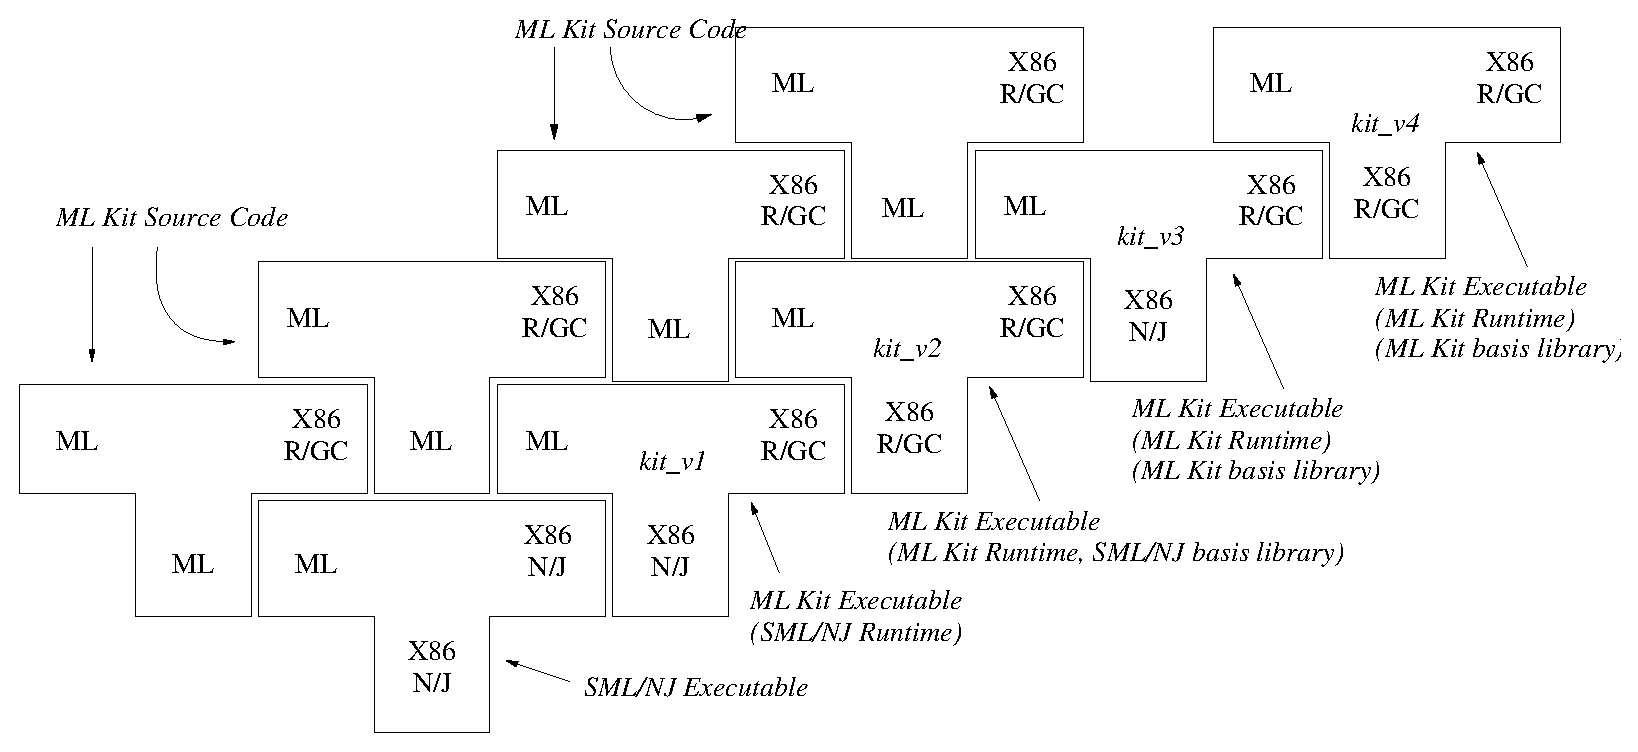
\includegraphics{bootstrap.eps}}
\end{center}
\caption{The bootstrapping process illustrated using T-diagrams. Each compiler 
  in the diagram is characterized by three languages: the source
  language that it compiles, the target language that it generates
  code for, and the implementation language that it is written in.}
\label{bootstrap.fig}
\medskip\hrule
\end{figure}

The lowest block in the picture denotes the SML/NJ compiler, which is
used to compile the ML Kit sources to a version of the ML Kit that,
when running, uses SML/NJ's runtime system. This version of the ML Kit
is pictured to the right of the SML/NJ executable and is named
\emph{kit\_v1}.

To build \emph{kit\_v1} 
\index{bootstrap!\emph{kit\_v1}}%
enter the directory \texttt{kit} (i.e., the directory containing the
file \texttt{copyright}). The \texttt{kit} directory contains a {\tt
  Makefile} that automates the bootstrapping process.  Assuming, that
the ML Kit is installed in the directory
\texttt{\$HOME/mlkit}, from within this directory,
type the following commands so as to generate the \emph{kit\_v1}
compiler:
\begin{verbatim}
  # make clean
  ...
  # make
  ...
\end{verbatim}

The {\tt make} command produces a file \texttt{bin/kit.x86-linux},
which is an SML/NJ image that can be executed using the shell script
\texttt{bin/mlkit}. The image is compiled using the Basis Library of
SML/NJ and executes using the runtime system of SML/NJ. We now install
\texttt{kit\_v1} in a new directory, say \texttt{mlkit-v1}:
\begin{verbatim}
  # make install INSTDIR=$HOME/mlkit-v1
  ...
  # unlimit stacksize
  # make bootstrap INSTDIR=$HOME/mlkit-v1
\end{verbatim}
These commands create the directory \texttt{mlkit-v1} with files
necessary to bootstrap and test \emph{kit\_v1}. The command
\index{unlimit stacksize}%
\texttt{unlimit stacksize} is necessary because the ML Kit stores lots
of data on the stack (i.e., in finite regions).

Compiling the ML Kit source with \emph{kit\_v1} generates
\index{bootstrap!\emph{kit\_v2}}%
\emph{kit\_v2}. The \emph{kit\_v2} executable runs on the runtime
system of the ML Kit using region inference. However, \emph{kit\_v2}
is still affected by SML/NJ, for instance, many constants including
bit-vectors are calculated using the Basis Library of SML/NJ.  Thus,
the \emph{kit\_v2} executable may work even if the ML Kit
implementation of the Basis Library is buggy.

Unfortunately, because of the engineering of the recompilation scheme
used in the ML Kit, it is not at present possible to memorize 
\label{memorize_bootstrap.sec}
the compilation of the Standard ML Basis Library
\index{bootstrap!Standard ML Basis Library}%
when using a bootstrapped version of the compiler (i.e.,
\emph{kit\_v2} $\ldots$ \emph{kit\_v4}), the Basis Library is compiled
every time a program is compiled.

Another reason that the two executables \emph{kit\_v2} and
\emph{kit\_v3} are different is that machine code labels are chosen
different when memorization of the Basis Library is used compared
to when memorization is not used.

To generate the \emph{kit\_v2} compiler, enter the directory
\texttt{mlkit-v1}. Here you find a {\tt Makefile} with a {\tt
  bootstrap} entry.  Using the {\tt bootstrap} entry (and specifying
the directory where \emph{kit\_v2} is to be installed) generates and
installs \texttt{kit\_v2}. This process may take several hours
depending on your machine:\footnote{Your machine should have at least
  1 Gb of RAM to avoid swapping during the entire bootstrapping
  process.}
\begin{verbatim}
  # cd $HOME/mlkit-v1
  ...
  # unlimit stacksize
  # make bootstrap INSTDIR=$HOME/mlkit-v2
\end{verbatim}
To generate 
\index{bootstrap!\emph{kit\_v3}}%
the \emph{kit\_v3} compiler, enter the \texttt{mlkit-v2} directory and
bootstrap once more by using the {\tt Makefile} located in
\texttt{mlkit-v2}:
\begin{verbatim}
  # cd $HOME/mlkit-v2
  # unlimit stacksize
  # make bootstrap INSTDIR=$HOME/mlkit-v3
  ...
\end{verbatim}
To generate 
\index{bootstrap!\emph{kit\_v4}}%
the \emph{kit\_v4} compiler, enter the \texttt{mlkit-v3} directory and
bootstrap yet another time by using the {\tt Makefile} located in
\texttt{mlkit-v3}:
\begin{verbatim}
  # cd $HOME/mlkit-v3
  # unlimit stacksize
  # make bootstrap INSTDIR=$HOME/mlkit-v4
  ...
\end{verbatim}
To see that the two executables \emph{kit\_v3} and \emph{kit\_v4} are
identical, you can apply the \texttt{diff} command on the two
binaries:
\begin{verbatim}
  # diff $HOME/mlkit-v3/bin/mlkit.img \
         $HOME/mlkit-v4/bin/mlkit.img
  #
\end{verbatim}

% # ll /import/home/nh/ITU/MLKit/mlkit-v3/bin/mlkit.img 
% ...  8867248 Jun  8 11:02 /import/.../mlkit-v3/bin/mlkit.img*

\section{Compiling the ML Kit with Itself}

To compile the ML Kit with the ML Kit, each {\tt Makefile} takes the
approach of launching the appropriate ML Kit compiler with the file 
\index{bootstrap!\texttt{sources.pm}}%
{\tt src/sources.pm} as argument. Assuming the ML Kit compiler is
launched from within the {\tt src} directory and that the compilation
works out fine, a new executable version of the ML Kit is available as
the file {\tt run} in the \texttt{src} directory:

%If you are using one of the versions: \emph{kit\_v2}, $\ldots$,
%\emph{kit\_v4} you must supply an install directory:

\begin{verbatim}
  # cd $HOME/mlkit-v3/src
  # ../bin/mlkit sources.pm
  ...
\end{verbatim}

% The install directory is necessary for the ML Kit to find the runtime
% system when building the executable file \texttt{run}.

\section{Testing the Bootstrapped Compiler}
\index{bootstrap!testing}%

It is possible to apply all the ML Kit tests in the test directory to
the bootstrapped versions of the ML Kit.  The regression test performs
a test on the following four configurations of the ML Kit:

\begin{enumerate}
\item with region inference alone
\item with region inference and profiling
\item with region inference and garbage collection
\item with region inference, garbage collection, and profiling
\end{enumerate}

To make a regression test of the \emph{kit\_v3} compiler, execute the
following commands:

\begin{verbatim}
  # cd $HOME/mlkit-v3
  # make all_test
  ...
\end{verbatim}
If you look in the \texttt{all\_test} entry in the {\tt Makefile}, you
find that the entry calls a program called \texttt{kittester} with a
file \texttt{all.tst} given as argument.  The file \texttt{all.tst}
contains information about the programs that are tested and under what configurations.
The program \texttt{kittester} performs the test, that is, each
program is compiled, executed and output is compared to the expected
output.  Finally a \LaTeX{} report with the result of the test is
written to the file \texttt{test\_report.dvi}.

When you inspect the test report \texttt{test\_report.dvi}, you may
notice that {\tt kittester} reports some errors (at the time of
writing 16 errors are reported but that may change as the test suite
is extended). All files resulting in compile time errors (option
\texttt{ecte} in file \texttt{all.tst}) are reported twice with an
error in \texttt{test\_report.dvi}. The errors are reported because
the Basis Library is compiled for each program and compiler output
therefore differs from expected compiler output (see the discussion
about memorization of the Basis Library on page
\pageref{memorize_bootstrap.sec}).

\section{Profiling the ML Kit}

The Kit can compile itself only when the compiler is produced with
garbage collection enabled.  The memory usage is similar for all the
ML Kit compilers generated during the bootstrapping process.

To profile the ML Kit, we generate a version of the ML Kit compiler
with profiling enabled; we call it 
\index{bootstrap!\emph{kit\_v4prof}}%
$\emph{kit\_v4prof}$ and build it using $\emph{kit}_{v4}$:
\begin{verbatim}
  # cd $HOME/mlkit-v4
  # unlimit stacksize
  # make bootstrap COMP_FLAGS=-prof INSTDIR=$HOME/mlkit-v4prof
  ...
\end{verbatim}
To generate a region profile of the ML Kit we use $\emph{kit\_v4prof}$
to compile a smaller program \texttt{kitkbjul9.sml} found in the
\texttt{test} directory of the source distribution. We enter the
\texttt{test} directory and compile \texttt{kitkbjul9.sml} using the
\texttt{mlkit} program (with profiling enabled), located in the
\texttt{bin} directory:

\begin{verbatim}
  # cd $HOME/mlkit-v4prof/test
  # unlimit stacksize
  # ../bin/mlkit kitkbjul9.sml
  ...
  [wrote executable file: run]
  # rp2ps -region -name "MLKit compiling kitkbjul9" \
         -sampleMax 2000 -eps 137 mm
  Region profiling to output file region.ps.
  Using name MLKit compiling kitkbjul9.
  Using 2000 samples.
  Using encapsulated postscript with width 388 pt.
  # gv -seascape region.ps
\end{verbatim}

Figure~\ref{mlkit_compiling_kitkbjul9.fig} shows the region
profile obtained with the commands shown above.
\begin{figure}
%\hrule \medskip
\begin{center}
\includegraphics{mlkit_compiling_kitkbjul9.eps}
\end{center}
\caption{A region profile of the ML Kit compiling the program \texttt{kitkbjul9.sml}, 
which is located in the \texttt{test} directory of the source distribution.}
\label{mlkit_compiling_kitkbjul9.fig}
\medskip\hrule
\end{figure}


\section{Controlling Profiling Options}

To control the profiling options at runtime as described in
Chapter~\ref{useOfProf.sec}, we use the program \texttt{mlkit.img} in
the \texttt{bin} directory and supply all command line parameters
necessary, which includes an install directory (i.e., the directory
specified when building this particular version of the ML Kit). You
can look in the file \texttt{bin/mlkit} to find the install directory.

The Figure~\ref{mlkit_compiling_kitkbjul9_400msec.fig} shows a region
profile similar to Figure~\ref{mlkit_compiling_kitkbjul9.fig} except
that the number of profile ticks is increased using the option
(\texttt{-microsec 100000}):

\begin{verbatim}
  # unlimit stacksize
  # cd $HOME/mlkit-v4prof/test
  # ../bin/mlkit.img -realtime -microsec 100000 \
    $HOME/mlkit-v4prof/ kitkbjul9.sml 
  ...
  [wrote executable file: run]
  # rp2ps -region -sampleMax 2000 -eps 137 mm \
          -name "MLKit compiling kitkbjul9 (100000 microsec)"         
  Region profiling to output file region.ps.
  Using name MLKit compiling kitkbjul9 (100000 microsec).
  Using 2000 samples.
  Using encapsulated postscript with width 388 pt.
  # gv -seascape region.ps
\end{verbatim}

\begin{figure}
%\hrule \medskip
\begin{center}
\includegraphics{mlkit_compiling_kitkbjul9_400msec.eps}
\end{center}
\caption{A region profile of the MLKit compiling the program \texttt{kitkbjul9.sml}. 
 Memory is traversed once every 0.1 second.}
\label{mlkit_compiling_kitkbjul9_400msec.fig}
%\medskip\hrule
\end{figure}

                                

%---------------------------------------------------------
\chapter{Summary of Changes}
%---------------------------------------------------------

\section{Changes Since Version 3}
\index{changes!since version 3}%
This chapter provides an overview of the main changes to the ML Kit
since version 3.0.

\subsubsection*{Garbage Collection}
\index{garbage collection}%
The ML Kit supports reference tracing garbage collection in
combination with the region memory model. Garbage collection is
supported only in the native backend version of the Kit. To enable
garbage collection, toggle the entry {\tt garbage collection} in the
{\tt Control} menu or start the Kit with the option {\tt -gc}. Garbage
collection is also possible with region profiling enabled. See
Chapter~\ref{gc.chap} for more information about garbage collection
with the Kit.

\subsubsection*{X86 Backend}
The 
\index{backend!hppa}%
HPPA backend of the ML Kit version 3.0 and earlier has been replaced
with an
\index{backend!x86}%
x86 native backend, which uses the GNU assembler to create native
machine code on x86 machines.

\subsubsection*{Bytecode Backend}
\index{backend!bytecode}%
For portability, the ML Kit now provides a bytecode backend and a
bytecode interpreter. Which backend is used by the ML Kit compiler is
determined when the Kit itself is compiled, but it is possible to have
both a native version and a bytecode version of the ML Kit compiler
installed on the same system.

\subsubsection*{Unboxing of Function Arguments}
\index{arguments!multiple}%
\index{multiple function arguments}%
\index{function arguments!multiple}%
By default, the Kit performs a simple local unboxing analysis to
figure out if a function taking a tuple as argument can be transformed
into a function taking multiple arguments. Only functions that use
only the individual elements of the argument tuple undergo
transformation. The optimisation can be disabled by toggling the entry
{\tt unbox function arguments} in the {\tt Control/Optimiser} menu.

\subsubsection*{Removal of Region Vectors}
\index{region vector!removed}%
In the ML Kit version 3.0 and earlier, actual region parameters were
passed to a region polymorphic function in a {\em region vector},
which itself was allocated in a region. In version 4.0, actual region
parameters to
\index{function!region polymorphic}%
region polymorphic functions are passed in registers and on the stack.
This simplification improves pretty printing of region annotated terms
and on what function calls turn into tail calls (see
Section~\ref{simplejump.sec}).

\section{Changes Since Version 2}
\index{changes!since version 2}%
This section provides an overview of the main changes to the ML Kit
since version 2.0 but before version 3.0 of the Kit.

\subsubsection*{Modules and Separate Compilation}
The most important development since Version 2 is the ability to
compile Modules and the discipline of separate compilation. A
distinguished feature of the way modules are compiled is that module
constructs do not give rise to any code, so there is no runtime
overhead in using modules \cite{ElsmanICFP99,ElsmanThesis}. See
Chapter~\ref{modules_and_projects.chap}.

\subsubsection*{Standard ML Basis Library}
The ML Kit now contains (a large portion of) the \index{Standard ML
  Basis Library} Standard ML Basis Library, based on the Moscow ML
version of the library. To see exactly what parts of the Standard ML
Basis Library are supported, consult the project file {\tt
  basislib.pm} located in the directory {\tt basislib}.

\subsubsection*{Scalability}
The Kit now compiles fairly large programs, including Hafnium's AnnoDomini
(58.000 lines of SML) and the ML Kit itself (around 80.000 lines).

\subsubsection*{New Match Compiler}
The pattern compiler has been rewritten, based on Sestoft's 
method~\cite{sestoft96}, which is also the basis of the Moscow ML 
match compiler. 

\subsubsection*{New StatObject Module}
The Kit contains a module, 
\index{StatObject}%
{\tt StatObject}, which implements the semantic objects of the static
semantics of the Core.  Originally, this was a very clean and very
inefficient implementation of the Defininion. In version 2 of the Kit,
{\tt StatObject} was replaced by an imperative and efficient, but
complicated module.  In version 3, {\tt StatObject} uses a clean,
efficient and imperative implementation of {\tt StatObject}. This is
particularly useful for those who want to reuse the front-end of the
Kit for other purposes.

\subsubsection*{Unboxed Representation of Lists}
\index{list} List constructors are now represented unboxed, that is,
the least significant bits of a list value is used to distinguish
between \boxml{nil} and a pointer to a pair (\boxml{::}) holding the
head and the tail of the list. Thus, a list takes up only one region
(for the auxiliary pairs) plus any regions for the elements of the
list. Consult Chapter~\ref{lists.sec} for details.

\nocite{total97,total94,btv96,elshal95,KochHojfeld96,H96,hallenberg99,brtt93}

\bibliographystyle{alpha}
\bibliography{tofte}

\appendix

%---------------------------------------------------------
\chapter{Command-Line Options}
\label{mlkithelp.app}
%---------------------------------------------------------
This appendix shows the output of executing 
\index{help@\texttt{-help} option to \texttt{mlkit}}%
\boxml{mlkit -help}, where \boxml{mlkit} is the version of the ML Kit
compiler that uses the 
\index{backend!x86}%
x86 native backend. The options are slightly different for the version
of the ML Kit compiler that uses the bytecode backend.

\begin{verbatim}
ML Kit version 4.0.0, Sep 20, 2001 [X86 Backend]

Usage: mlkit [OPTION]... [file.sml | file.sig | file.pm]

Options:

-script file
     Read compiler options from `file'.

-version
     Print ML Kit version information and exit.

-help s
     Print help information about an option and exit.

-help
     Print help information and exit.

--all_multiplicities_infinite                             (off)
     Use only infinite regions. That is, store all values in
     infinite regions, which do not reside on the stack, but
     in the heap. With this flag disabled, all regions that
     can be inferred that values are allocated in them at
     most once are allocated on the stack.

--chat, -verbose                                          (off)
     Print a message for each compilation step in the compiler.

--clibs S                                           ("-lm -lc")
     If you have added your own object files to a project,
     you might also need to link with libraries other
     than libm.a and libc.a ("-lm -lc").

--comments_in_x86_asmcode                                 (off)
     Insert comments in x86 assembler code.

--compiler_timings, -timings                              (off)
     Show compiler timings for each compilation phase.

--contract                                                 (on)
     Contract is responsible for in-lining, specialization,
     elimination of dead code, and much else (Lambda
     Expression Optimiser).

--no_contract
     Opposite of --contract.

--debug_compiler, -debug                                  (off)
     Print intermediate forms of a program during compilation.

--debug_linking                                           (off)
     Debug linking of target code by showing which object
     files are linked together.

--debug_man_enrich                                        (off)
     During interactive use, show information about why a
     program unit need be recompiled. In the ML Kit, a
     program unit (or a functor body) is recompiled if
     either (a) the program unit is modified, or (b)
     information about an identifier for which the program
     unit depends upon has changed.

--debug_which_at                                          (off)
     Debug storage mode analysis.

--delete_target_files                                      (on)
     Delete assembler files produced by the compiler. If you
     disable this flag, you can inspect the assembler code
     produced by the compiler.

--no_delete_target_files
     Opposite of --delete_target_files.

--disable_atbot_analysis                                  (off)
     Disable storage mode analysis. That is, turn all
     allocation directives into attop.

--disable_flow_var                                        (off)

--eliminate_explicit_records                               (on)
     Eliminate bindings of explicit records only used for
     selections. Transform
           let r = (e1,...,en) in ... #i r .. #j r ...
     into
           let x1=e1 in ... let xn=en in ... xi .. xj ...
     (Lambda Expression Optimiser).

--no_eliminate_explicit_records
     Opposite of --eliminate_explicit_records.

--garbage_collection, -gc                                 (off)
     Enable garbage collection. When enabled, regions are
     garbage collected during execution of the program. When
     garbage collection is enabled, all values are tagged. Due
     to region inference, for most programs, the garbage
     collector is invoked less often than for systems based
     only on garbage collection.

--no_garbage_collection, -no_gc
     Opposite of --garbage_collection, -gc.

--gdb_support, -g                                         (off)
     When enabled, the compiler passes the option --gstabs
     to `as' (The GNU Assembler) and preserves the generated
     assembler files (.s files). Passing the --gstabs
     option to `as' makes it possible to step through
     the generated program using gdb (The GNU Debugger).

--import_basislib, -basislib                               (on)
     Import Basis Library automatically in your projects. If 
     you wish to make use of the Standard ML Basis Library
     in your projects, this option should be turned on, unless
     you wish to import the Basis Library manually in your
     projects.

--no_import_basislib, -no_basislib
     Opposite of --import_basislib, -basislib.

--install_dir S                            ("/usr/share/mlkit")
     Installation directory for the ML Kit. For normal
     execution you should not modify this value. However,
     if you wish to use the ML Kit with an altered runtime
     system and you do not wish to exchange the .o-files in
     the bin-subdirectory (for example because you are running
     the ML Kit on a shared system), you can update this
     setting and the system will try to link to a runtime
     system in the bin-subdirectory found in the new install
     directory.

--keep_functor_bodies_in_memory                           (off)
     With this flag enabled, functor bodies are kept in
     memory, for the compilation of future applications of
     the functors. Keeping functor bodies in memory causes
     the memory consumptions of the compiler to grow
     dramatically. With the flag disabled (which is the
     default), the compiler writes the functor body to disk
     and reparses and reelaborates the functor body for each
     application. Reelaboration is necessary because the
     compiler uses type information in many of its backend
     phases.

--log_to_file                                             (off)
     Log to files instead of stdout.

--maximum_inline_size N                                    (20)
     Functions smaller than this size (counted in abstract
     syntax tree nodes) are in-lines, even if they are used
     more than once. Functions that are used only once are
     always in-lined.

--maximum_specialise_size N                               (200)
     Curried functions smaller than this size (counted in
     abstract syntax tree nodes) are specialised if all
     applications of the function within its own body are
     applied to its formal argument, even if they are used
     more than once. Functions that are used only once are
     specialised no matter their size. See also the option
     --specialize_recursive_functions.

--minimize_fixs                                            (on)
     Minimize fix constructs (Lambda Expression Optimiser).

--no_minimize_fixs
     Opposite of --minimize_fixs.

--optimiser, -opt                                          (on)
     Enable optimisation of intermediate language code
     (Lambda Expressions). Which optimisations are performed
     is controlled by individual flags. The optimisations
     include function in-lining, function specialisation,
     fix-minimization, unboxing of function arguments, and
     elimination of unnecessary record constructions.

--no_optimiser, -no_opt
     Opposite of --optimiser, -opt.

--output S, -o S                                        ("run")
     The name of the executable file generated by
     the Kit.

--print_K_normal_forms                                    (off)
     Print Region Expressions in K-Normal Form. Applicable,
     only after storage mode analysis has been applied.

--print_all_program_points, -Ppp                          (off)
     Print all program points when printing physical size
     inference expressions. Use the menu item
     ``print program points'' to print only some program
     points.

--print_bit_vectors                                       (off)

--print_calc_offset_program                               (off)

--print_call_explicit_expression, -Pcee                   (off)
     Print Region Expression with call annotations.

--print_clos_conv_program, -Pccp                          (off)
     Print Region Expression after closure conversion.

--print_drop_regions_expression, -Pdre                    (off)
     Print Region Expression after dropping word regions and
     regions arguments with only get-effects.

--print_drop_regions_expression_with_storage_modes, -Pdresm (off)
     Print Region Expression after dropping word regions and
     regions arguments with only get-effects. Also print
     atbot and attop annotations resulting from storage mode
     analysis.

--print_effects, -Peffects                                (off)
     Print effects in region types.

--print_fetch_and_flush_program                           (off)
     Print program with instructions for activation
     record fetching and flushing.

--print_lift_conv_program, -Plcp                          (off)
     Print Region Expression after lifting. Used for the
     compilation into byte code (KAM).

--print_linearised_program                                (off)

--print_normalized_program                                (off)
     Print Region Expression after K-normalisation.

--print_opt_lambda_expression, -Pole                      (off)
     Print Lambda Expression after optimisation.

--print_physical_size_inference_expression, -Ppse         (off)
     Print Region Expression after physical size inference.

--print_region_flow_graph, -Prfg                          (off)
     Print a region flow graph for the program fragment
     and generate a .vcg-file, which can be viewed using
     the xvcg program.

--print_regions, -Pregions                                 (on)
     Print region variables in types and expressions.

--no_print_regions, -no_Pregions
     Opposite of --print_regions, -Pregions.

--print_register_allocated_program                        (off)

--print_rho_levels                                        (off)
     Print levels of region and effect variables in types and
     intermediate forms. Levels control quantification of
     region and effect variables.

--print_rho_types                                         (off)
     Print region types of region variables in types and
     intermediate forms. Possible region types are:
         w   type of regions containing only word values; these
             regions are dropped from the program because word
             values are represented unboxed.
         r   type of regions containing only reals.
         s   type of regions containing only strings.
         t   type of regions not containing word values, reals,
             or strings.

--print_simplified_program                                (off)
     Print simplified program after register
     allocation.

--print_storage_mode_expression, -Psme                    (off)
     Print Region Expression after storage mode analysis

--print_type_name_stamps, -Ptypestamps                    (off)
     Print type name stamps and their attributes in types
     and expressions.

--print_types, -Ptypes                                    (off)
     Print types when printing intermediate forms. For Lambda
     Expressions, ordinary ML types are printed, whereas for
     Region Expressions, region types are printed.

--print_word_regions, -Pwordregions                       (off)
     Also print word regions that have been dropped.

--quotation, -quot                                        (off)
     Enable support for quotations and anti-quotations.
     When enabled, the datatype
        datatype 'a frag = QUOTE of string
                         | ANTIQUOTE 'a
     is available in the initial environment. Moreover,
     values of this datatype may be constructed using
     the quotation/antiquotation syntax:
        val s = "world" 
        val a : string frag list = `hello ^s - goodbye`

--raggedRight                                              (on)
     Use ragged right margin in pretty-printing of
     expressions and types.

--no_raggedRight
     Opposite of --raggedRight.

--region_profiling, -prof                                 (off)
     Enable region profiling. Object code stemming
     from compiling a program with region profiling enabled
     is instrumented with profiling information. When a program
     compiled with region profiling enabled is run, the program
     produces a profile file run.rp, which can then be read
     by the profiling tool rp2ps that comes with the ML Kit to
     produce profiling graphs of various forms.

--register_allocation                                      (on)
     Perform register allocation. Without register allocation
     enabled, programs run somewhat slower--but they run andn
     you save about 15 percent on compile time.

--no_register_allocation
     Opposite of --register_allocation.

--report_file_sig, -sig                                   (off)
     Report signatures for each file read.

--specialize_recursive_functions                           (on)
     Specialise recursive functions. Use the option
     maximum_specialise_size to control which functions
     are specialised. If this flag is on, functions that are
     applied only once are specialised, no matter the setting
     of maximum_specialise_size (Lambda Expression Optimiser).

--no_specialize_recursive_functions
     Opposite of --specialize_recursive_functions.

--statistics_after_optimisation                           (off)
     Report optimisation statistics after optimisation of
     Lambda Expression.

--strip                                                   (off)
     If enabled, the Kit strips the generated executable.

--type_check_lambda                                        (on)
     Type check lambda expression prior to performing region
     inference. Type checking is very fast and for normal use
     you should not disable this option. Type checking
     intermediate forms is very powerful for eliminating bugs
     in the compiler.

--no_type_check_lambda
     Opposite of --type_check_lambda.

--unbox_function_arguments                                 (on)
     Unbox arguments to fix-bound functions, for which the
     argument `a' is used only in contexts `#i a'. All call 
     sites are transformed to match the new function (Lambda
     Expression Optimiser).

--no_unbox_function_arguments
     Opposite of --unbox_function_arguments.

--warn_on_escaping_puts                                   (off)
     Enable the compiler to issue a warning whenever a 
     region type scheme contains a put effect on a region
     that is not quantified.

--width N, -w N                                           (100)
     Column width used when pretty printing intermediate code.
\end{verbatim}

\newpage
\index{live variable analysis|see{variable}}
\index{endomorphism|see{region endomorphism}}
\index{exomorphism|see{region exomorphism}}
\index{tuple|see{record}}
\index{$\mu$|see{type and place}}
\index{rDesc|see{region descriptor}}
\index{example programs|see{{\tt kitdemo} directory}}
\index{value declaration|see{declaration}}
\printindex

\newpage
\begin{center}
\bf Global Regions
\end{center}
\smallskip

\hrule
\halign{\parbox[t]{15mm}{#}\hfil\ &\ \parbox[t]{13cm}{\strut#\strut}\cr
\boxml{r1}&Holds values of type {\tt top}, that is, records, exceptions, and closures.\cr
\boxml{r2}&This region does not actually exist; it is used with unboxed values,
           such as integers, booleans, and the 0-tuple.\cr
\boxml{r3}&Holds values of type {\tt bot}. Because no values has type 
{\tt bot}, this region contains no values. Region variables with region type {\tt bot} are used with
type variables.\cr
\boxml{r4}&Holds values of type {\tt string}.\cr
\boxml{r5}&Holds values of type {\tt real}.\cr
}
\hrule
\bigskip
\end{document}

